\documentclass[twoside]{book}

% Packages required by doxygen
\usepackage{fixltx2e}
\usepackage{calc}
\usepackage{doxygen}
\usepackage[export]{adjustbox} % also loads graphicx
\usepackage{graphicx}
\usepackage[utf8]{inputenc}
\usepackage{makeidx}
\usepackage{multicol}
\usepackage{multirow}
\PassOptionsToPackage{warn}{textcomp}
\usepackage{textcomp}
\usepackage[nointegrals]{wasysym}
\usepackage[table]{xcolor}

% NLS support packages
\usepackage{hfont}

% Font selection
\usepackage[T1]{fontenc}
\usepackage[scaled=.90]{helvet}
\usepackage{courier}
\usepackage{amssymb}
\usepackage{sectsty}
\renewcommand{\familydefault}{\sfdefault}
\allsectionsfont{%
  \fontseries{bc}\selectfont%
  \color{darkgray}%
}
\renewcommand{\DoxyLabelFont}{%
  \fontseries{bc}\selectfont%
  \color{darkgray}%
}
\newcommand{\+}{\discretionary{\mbox{\scriptsize$\hookleftarrow$}}{}{}}

% Page & text layout
\usepackage{geometry}
\geometry{%
  a4paper,%
  top=2.5cm,%
  bottom=2.5cm,%
  left=2.5cm,%
  right=2.5cm%
}
\tolerance=750
\hfuzz=15pt
\hbadness=750
\setlength{\emergencystretch}{15pt}
\setlength{\parindent}{0cm}
\setlength{\parskip}{3ex plus 2ex minus 2ex}
\makeatletter
\renewcommand{\paragraph}{%
  \@startsection{paragraph}{4}{0ex}{-1.0ex}{1.0ex}{%
    \normalfont\normalsize\bfseries\SS@parafont%
  }%
}
\renewcommand{\subparagraph}{%
  \@startsection{subparagraph}{5}{0ex}{-1.0ex}{1.0ex}{%
    \normalfont\normalsize\bfseries\SS@subparafont%
  }%
}
\makeatother

% Headers & footers
\usepackage{fancyhdr}
\pagestyle{fancyplain}
\fancyhead[LE]{\fancyplain{}{\bfseries\thepage}}
\fancyhead[CE]{\fancyplain{}{}}
\fancyhead[RE]{\fancyplain{}{\bfseries\leftmark}}
\fancyhead[LO]{\fancyplain{}{\bfseries\rightmark}}
\fancyhead[CO]{\fancyplain{}{}}
\fancyhead[RO]{\fancyplain{}{\bfseries\thepage}}
\fancyfoot[LE]{\fancyplain{}{}}
\fancyfoot[CE]{\fancyplain{}{}}
\fancyfoot[RE]{\fancyplain{}{\bfseries\scriptsize 다음에 의해 생성됨 \+:  Doxygen }}
\fancyfoot[LO]{\fancyplain{}{\bfseries\scriptsize 다음에 의해 생성됨 \+:  Doxygen }}
\fancyfoot[CO]{\fancyplain{}{}}
\fancyfoot[RO]{\fancyplain{}{}}
\renewcommand{\footrulewidth}{0.4pt}
\renewcommand{\chaptermark}[1]{%
  \markboth{#1}{}%
}
\renewcommand{\sectionmark}[1]{%
  \markright{\thesection\ #1}%
}

% Indices & bibliography
\usepackage{natbib}
\usepackage[titles]{tocloft}
\setcounter{tocdepth}{3}
\setcounter{secnumdepth}{5}
\makeindex

% Hyperlinks (required, but should be loaded last)
\usepackage{ifpdf}
\ifpdf
  \usepackage[pdftex,pagebackref=true]{hyperref}
\else
  \usepackage[ps2pdf,pagebackref=true]{hyperref}
\fi
\hypersetup{%
  colorlinks=true,%
  linkcolor=blue,%
  citecolor=blue,%
  unicode%
}

% Custom commands
\newcommand{\clearemptydoublepage}{%
  \newpage{\pagestyle{empty}\cleardoublepage}%
}

\usepackage{caption}
\captionsetup{labelsep=space,justification=centering,font={bf},singlelinecheck=off,skip=4pt,position=top}

%===== C O N T E N T S =====

\begin{document}

% Titlepage & ToC
\hypersetup{pageanchor=false,
             bookmarksnumbered=true,
             pdfencoding=unicode
            }
\pagenumbering{roman}
\begin{titlepage}
\vspace*{7cm}
\begin{center}%
{\Large cvtdriver }\\
\vspace*{1cm}
{\large 다음에 의해 생성됨 \+:  Doxygen 1.8.11}\\
\end{center}
\end{titlepage}
\clearemptydoublepage
\tableofcontents
\clearemptydoublepage
\pagenumbering{arabic}
\hypersetup{pageanchor=true}

%--- Begin generated contents ---
\chapter{Converting Driver for Smart\+Farm Devices}
\label{index}\hypertarget{index}{}\section*{cvtdriver}

cvtdriver 는 \href{https://github.com/ebio-snu/stdcvt}{\tt 스마트팜장비 연동을 위한 컨버터 개발} 프로젝트에서 활용되는 드라이버개발을 돕기 위한 프로젝트이다. 본 프로젝트에서 드라이버 개발을 위한 A\+PI 스펙 및 샘플 드라이버를 제공하여 참여사의 드라이버 제작을 돕는다.

\subsection*{클래스 구조}

드라이버 클래스 구조는 다음과 같다.




\begin{DoxyItemize}
\item \hyperlink{classstdcvt_1_1CvtDriver}{Cvt\+Driver} \+: 드라이버의 인터페이스가 되는 가상 클래스이다.
\item \hyperlink{classstdcvt_1_1CvtOption}{Cvt\+Option} \+: 드라이버 구동을 위한 옵션을 전달하는 클래스이다.
\item \hyperlink{classstdcvt_1_1CvtDeviceSpec}{Cvt\+Device\+Spec} \+: 드라이버에서 다루는 장비의 스펙을 다루는 클래스이다. 장비종류, 설치위치, 장비의 작동대상, 제조사, 모델명을 처리한다.
\item \hyperlink{classstdcvt_1_1CvtDevice}{Cvt\+Device} \+: 드라이버에서 다루는 장비의 인터페이스가 되는 가상 클래스이다.
\begin{DoxyItemize}
\item \hyperlink{classstdcvt_1_1CvtSensor}{Cvt\+Sensor} \+: 센서의 인터페이스가 되는 클래스이다. 간단한 경우라면 직접 사용이 가능하다.
\item \hyperlink{classstdcvt_1_1CvtActuator}{Cvt\+Actuator} \+: 일반 구동기의 인터페이스가 되는 클래스이다. 스위치형 구동기에 사용하면 된다.
\item \hyperlink{classstdcvt_1_1CvtMotor}{Cvt\+Motor} \+: 모터형 구동기의 인터페이스가 되는 클래스로 Cvt\+Actuator를 상속한다. 간단한 경우라면 직접 사용이 가능하다.
\end{DoxyItemize}
\item \hyperlink{classstdcvt_1_1CvtCommand}{Cvt\+Command} \+: 구동기에서 처리하는 명령의 인터페이스가 되는 클래스이다.
\begin{DoxyItemize}
\item \hyperlink{classstdcvt_1_1CvtRatioCommand}{Cvt\+Ratio\+Command} \+: 구동기 전달하는 명령이 비율(퍼센트)인 경우에 사용하는 클래스이다. 모터형 구동기에 적합한 명령클래스라고 할 수 있다.
\end{DoxyItemize}
\end{DoxyItemize}

\subsection*{샘플 드라이버}

두가지 종류의 샘플드라이버를 제공한다.


\begin{DoxyItemize}
\item \hyperlink{classebiodriver_1_1DSSampleDriver}{D\+S\+Sample\+Driver} \+: 별도로 제공되는 샘플 노드와 serial 통신을 수행하는 드라이버이다. boost\+::asio 를 사용한다.
\item \hyperlink{classebiodriver_1_1SSSampleDriver}{S\+S\+Sample\+Driver} \+: 별도로 제공되는 테스트\+U\+I와 연동되는 드라이버이다. (현재는 구현이 안되어있다.) 
\end{DoxyItemize}
\chapter{코드표}
\label{md_doc_code_table}
\hypertarget{md_doc_code_table}{}
스마트팜 기기의 원활한 연동을 위해서 별도의 문서를 통해 공통 코드를 공유한다. 해당 문서는 지속적으로 업데이트 될 예정이며, 하위호환성을 최대한 유지할 계획이다. 공통코드는 장비의 상태, 장비의 종류, 장비의 설치위치, 관측치의 단위 등이다.


\begin{DoxyItemize}
\item 장비 상태
\item 장비 종류
\item 장비 설치 구역
\item 장비 작동 대상
\item 관측치 단위
\item 에러코드
\item 개발사번호 
\end{DoxyItemize}
\chapter{드라이버 A\+PI}
\label{md_doc_driver_api}
\hypertarget{md_doc_driver_api}{}
드라이버는 크게 2종류로 구분된다. 센서노드, 제어노드, 컨트롤러와 직접 연결되는 장비측(\+Device Side)드라이버와 데이터 수집기와 연결되는 서버측(\+Servier Side)드라이버로 구성된다. 각 드라이버를 D\+S\+Driver, S\+S\+Driver 라고 한다.

드라이버 A\+P\+I는 기초연동용과 고급연동용으로 구분될 계획이다. 현 단계에서 드라이버는 현상황을 충실히 포함하는쪽으로 설계하는 것을 목표로 하고 있다. 추후에 활성화가 되어 추상화 레벨을 높여서 더 많은 범위를 커버할 수 있기를 바란다.

\subsection*{드라이버 A\+PI 스펙 문서}

현 시점에서 기초 연동을 위한 A\+PI 초안이 개발되어 있으며, 참여사와의 워크샵을 통해 기초 연동용 최종안이 개발될 것으로 기대된다.


\begin{DoxyEnumerate}
\item \href{https://ebio-snu.github.io/cvtdriver/}{\tt 기초 연동 A\+PI 초안}
\end{DoxyEnumerate}
\begin{DoxyEnumerate}
\item \mbox{[}개발자 워크샵 수정안\mbox{]}()
\end{DoxyEnumerate}
\begin{DoxyEnumerate}
\item \mbox{[}기초 연동 A\+PI 최종안\mbox{]}() \+: A\+PI 버전 1.\+00
\end{DoxyEnumerate}
\begin{DoxyEnumerate}
\item \mbox{[}고급 연동 A\+PI 초안\mbox{]}()
\end{DoxyEnumerate}
\begin{DoxyEnumerate}
\item \mbox{[}고급 연동 A\+PI 최종안\mbox{]}() \+: A\+PI 버전 2.\+00
\end{DoxyEnumerate}

\subsection*{드라이버 클래스}

드라이버는 Cvt\+Driver 클래스를 상속받아 구현한다. 드라이버 클래스 다이어그램은 다음과 같다. 

\subsection*{드라이버가 가진 장비 데이터의 공유}

2개 이상의 D\+S\+Driver를 사용하는 경우 개별 D\+S\+Driver는 서로 다른 장비를 관리해야한다. 하나의 D\+S\+Driver에서 관리되는 장비에 대한 정보는 다른 장비로 전달될 수 있다.

드라이버로부터 장비 정보를 획득하기 위해서는 Cvt\+Device $\ast$getdevice(int index); 메소드를 활용한다. index는 0부터 시작하고, 값을 하나씩 올려가면서 장비를 꺼낼 수 있다. 이때 리턴값이 nullptr(\+N\+U\+L\+L)인 경우 관리하는 장비가 더이상 없다는 의미이다.

장비의 정보를 다른 드라이버로 전달하기 위해서 bool sharedevice(\+Cvt\+Device $\ast$pdevice); 메소드를 활용한다.

\subsection*{다른 드라이버로 제어명령 전달}

장비에 대한 명령도 다른 드라이버로 전달될 수 있다. 다만 초기버전에서는 S\+S\+Driver가 하나만 존재하고, S\+S\+Driver에서만 명령을 전달할 수 있는 것으로한다.

하나의 드라이버(\+S\+S\+Driver)가 전달하고자 하는 명령은 Cvt\+Command $\ast$getcommand(int index); 메소드를 이용해 얻을 수 있다. index는 0부터 시작하고, 값을 하나씩 올려가면서 명령을 꺼낼 수 있다. 이때 리턴값이 nullptr(\+N\+U\+L\+L)인 경우 더이상의 명령이 없다는 의미이다.

획득한 명령을 다른 드라이버로 전달하기 위해서 bool control(\+Cvt\+Command $\ast$pcmd); 메소드를 활용한다. 
\chapter{계통도 색인}
\section{클래스 계통도}
이 상속 목록은 완전하진 않지만 알파벳순으로 대략적으로 정렬되어있습니다.\+:\begin{DoxyCompactList}
\item \contentsline{section}{stdcvt\+:\+:Cvt\+Command}{\pageref{classstdcvt_1_1CvtCommand}}{}
\begin{DoxyCompactList}
\item \contentsline{section}{stdcvt\+:\+:Cvt\+Ratio\+Command}{\pageref{classstdcvt_1_1CvtRatioCommand}}{}
\item \contentsline{section}{stdcvt\+:\+:Cvt\+Raw\+Command}{\pageref{classstdcvt_1_1CvtRawCommand}}{}
\end{DoxyCompactList}
\item \contentsline{section}{stdcvt\+:\+:Cvt\+Device}{\pageref{classstdcvt_1_1CvtDevice}}{}
\begin{DoxyCompactList}
\item \contentsline{section}{stdcvt\+:\+:Cvt\+Actuator}{\pageref{classstdcvt_1_1CvtActuator}}{}
\begin{DoxyCompactList}
\item \contentsline{section}{ebiodriver\+:\+:S\+S\+Switch}{\pageref{classebiodriver_1_1SSSwitch}}{}
\item \contentsline{section}{stdcvt\+:\+:Cvt\+Motor}{\pageref{classstdcvt_1_1CvtMotor}}{}
\begin{DoxyCompactList}
\item \contentsline{section}{ebiodriver\+:\+:S\+S\+Motor}{\pageref{classebiodriver_1_1SSMotor}}{}
\end{DoxyCompactList}
\end{DoxyCompactList}
\item \contentsline{section}{stdcvt\+:\+:Cvt\+Sensor}{\pageref{classstdcvt_1_1CvtSensor}}{}
\begin{DoxyCompactList}
\item \contentsline{section}{ebiodriver\+:\+:S\+S\+Sensor}{\pageref{classebiodriver_1_1SSSensor}}{}
\end{DoxyCompactList}
\end{DoxyCompactList}
\item \contentsline{section}{stdcvt\+:\+:Cvt\+Device\+Spec}{\pageref{classstdcvt_1_1CvtDeviceSpec}}{}
\item \contentsline{section}{stdcvt\+:\+:Cvt\+Driver}{\pageref{classstdcvt_1_1CvtDriver}}{}
\begin{DoxyCompactList}
\item \contentsline{section}{ebiodriver\+:\+:D\+S\+Sample\+Driver}{\pageref{classebiodriver_1_1DSSampleDriver}}{}
\item \contentsline{section}{ebiodriver\+:\+:S\+S\+Sample\+Driver}{\pageref{classebiodriver_1_1SSSampleDriver}}{}
\end{DoxyCompactList}
\item \contentsline{section}{stdcvt\+:\+:Cvt\+Option}{\pageref{classstdcvt_1_1CvtOption}}{}
\item \contentsline{section}{stdcvt\+:\+:Cvt\+Spec}{\pageref{classstdcvt_1_1CvtSpec}}{}
\end{DoxyCompactList}

\chapter{데이타 구조 색인}
\section{데이타 구조}
다음은 데이타 구조들입니다. (간략한 설명만을 보여줍니다) \+:\begin{DoxyCompactList}
\item\contentsline{section}{\hyperlink{classstdcvt_1_1CvtActuator}{stdcvt\+::\+Cvt\+Actuator} }{\pageref{classstdcvt_1_1CvtActuator}}{}
\item\contentsline{section}{\hyperlink{classstdcvt_1_1CvtCommand}{stdcvt\+::\+Cvt\+Command} }{\pageref{classstdcvt_1_1CvtCommand}}{}
\item\contentsline{section}{\hyperlink{classstdcvt_1_1CvtDevice}{stdcvt\+::\+Cvt\+Device} }{\pageref{classstdcvt_1_1CvtDevice}}{}
\item\contentsline{section}{\hyperlink{classstdcvt_1_1CvtDeviceSpec}{stdcvt\+::\+Cvt\+Device\+Spec} }{\pageref{classstdcvt_1_1CvtDeviceSpec}}{}
\item\contentsline{section}{\hyperlink{classstdcvt_1_1CvtDriver}{stdcvt\+::\+Cvt\+Driver} }{\pageref{classstdcvt_1_1CvtDriver}}{}
\item\contentsline{section}{\hyperlink{classstdcvt_1_1CvtMotor}{stdcvt\+::\+Cvt\+Motor} }{\pageref{classstdcvt_1_1CvtMotor}}{}
\item\contentsline{section}{\hyperlink{classstdcvt_1_1CvtOption}{stdcvt\+::\+Cvt\+Option} }{\pageref{classstdcvt_1_1CvtOption}}{}
\item\contentsline{section}{\hyperlink{classstdcvt_1_1CvtRatioCommand}{stdcvt\+::\+Cvt\+Ratio\+Command} }{\pageref{classstdcvt_1_1CvtRatioCommand}}{}
\item\contentsline{section}{\hyperlink{classstdcvt_1_1CvtRawCommand}{stdcvt\+::\+Cvt\+Raw\+Command} }{\pageref{classstdcvt_1_1CvtRawCommand}}{}
\item\contentsline{section}{\hyperlink{classstdcvt_1_1CvtSensor}{stdcvt\+::\+Cvt\+Sensor} }{\pageref{classstdcvt_1_1CvtSensor}}{}
\item\contentsline{section}{\hyperlink{classstdcvt_1_1CvtSpec}{stdcvt\+::\+Cvt\+Spec} }{\pageref{classstdcvt_1_1CvtSpec}}{}
\item\contentsline{section}{\hyperlink{classebiodriver_1_1DSSampleDriver}{ebiodriver\+::\+D\+S\+Sample\+Driver} }{\pageref{classebiodriver_1_1DSSampleDriver}}{}
\item\contentsline{section}{\hyperlink{classebiodriver_1_1SSMotor}{ebiodriver\+::\+S\+S\+Motor} }{\pageref{classebiodriver_1_1SSMotor}}{}
\item\contentsline{section}{\hyperlink{classebiodriver_1_1SSSampleDriver}{ebiodriver\+::\+S\+S\+Sample\+Driver} }{\pageref{classebiodriver_1_1SSSampleDriver}}{}
\item\contentsline{section}{\hyperlink{classebiodriver_1_1SSSensor}{ebiodriver\+::\+S\+S\+Sensor} }{\pageref{classebiodriver_1_1SSSensor}}{}
\item\contentsline{section}{\hyperlink{classebiodriver_1_1SSSwitch}{ebiodriver\+::\+S\+S\+Switch} }{\pageref{classebiodriver_1_1SSSwitch}}{}
\end{DoxyCompactList}

\chapter{파일 색인}
\section{파일 목록}
다음은 문서화된 모든 파일에 대한 목록입니다. (간략한 설명만을 보여줍니다) \+:\begin{DoxyCompactList}
\item\contentsline{section}{sample/\hyperlink{dssampledriver_8cpp}{dssampledriver.\+cpp} }{\pageref{dssampledriver_8cpp}}{}
\item\contentsline{section}{sample/\hyperlink{sssampledriver_8cpp}{sssampledriver.\+cpp} }{\pageref{sssampledriver_8cpp}}{}
\item\contentsline{section}{spec/\hyperlink{cvtcode_8h}{cvtcode.\+h} }{\pageref{cvtcode_8h}}{}
\item\contentsline{section}{spec/\hyperlink{cvtcommand_8h}{cvtcommand.\+h} }{\pageref{cvtcommand_8h}}{}
\item\contentsline{section}{spec/\hyperlink{cvtdevice_8h}{cvtdevice.\+h} }{\pageref{cvtdevice_8h}}{}
\item\contentsline{section}{spec/\hyperlink{cvtdevicespec_8h}{cvtdevicespec.\+h} }{\pageref{cvtdevicespec_8h}}{}
\item\contentsline{section}{spec/\hyperlink{cvtdriver_8h}{cvtdriver.\+h} }{\pageref{cvtdriver_8h}}{}
\item\contentsline{section}{spec/\hyperlink{cvtoption_8h}{cvtoption.\+h} }{\pageref{cvtoption_8h}}{}
\end{DoxyCompactList}

\chapter{데이타 구조 문서화}
\hypertarget{classstdcvt_1_1CvtActuator}{}\section{stdcvt\+:\+:Cvt\+Actuator 클래스 참조}
\label{classstdcvt_1_1CvtActuator}\index{stdcvt\+::\+Cvt\+Actuator@{stdcvt\+::\+Cvt\+Actuator}}
stdcvt\+:\+:Cvt\+Actuator에 대한 상속 다이어그램 \+: \begin{figure}[H]
\begin{center}
\leavevmode
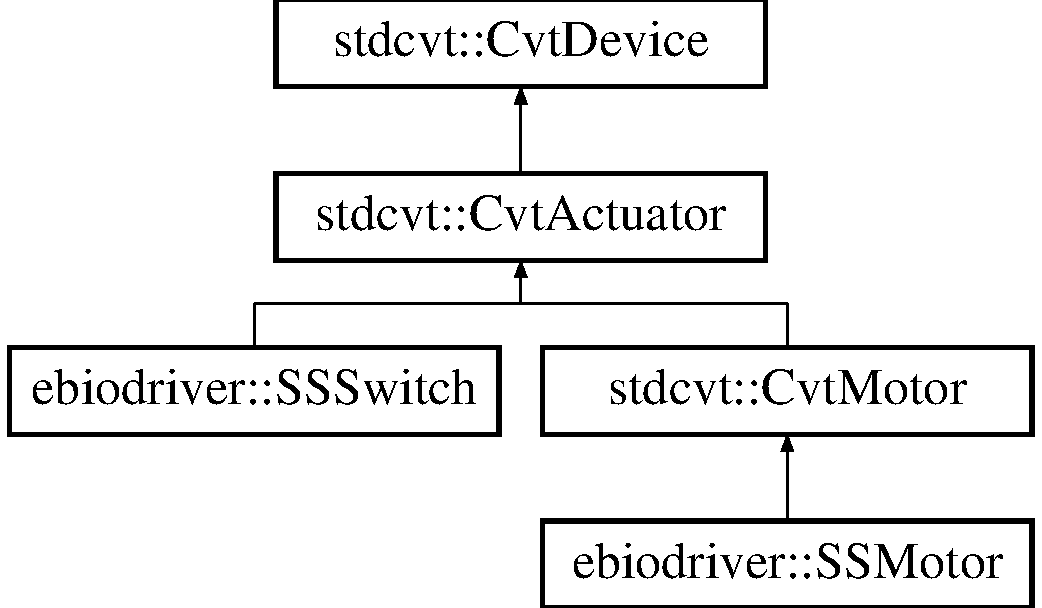
\includegraphics[height=4.000000cm]{classstdcvt_1_1CvtActuator}
\end{center}
\end{figure}
\subsection*{Public 멤버 함수}
\begin{DoxyCompactItemize}
\item 
\hyperlink{classstdcvt_1_1CvtActuator_a6e634ccf55c518a0c024200ba6d1bef8}{Cvt\+Actuator} (string devid, \hyperlink{cvtcode_8h_ae8e34073e35cef0bb47c7fa535fc638b}{devtype\+\_\+t} devtype, \hyperlink{cvtcode_8h_a268eebb73363e24b9e65fd51973bd9c0}{devsec\+\_\+t} section, \hyperlink{cvtcode_8h_a2b37fd5cc4d40c0b8c4b987c271e5ceb}{devtarget\+\_\+t} target, \hyperlink{cvtcode_8h_ad21cd565f839adc5b19a0993e7da7278}{devstat\+\_\+t} devstatus)
\item 
int \hyperlink{classstdcvt_1_1CvtActuator_a2e9fb1b6464f765d33b2a3b9f1abb0d1}{getlastcmdid} ()
\item 
bool \hyperlink{classstdcvt_1_1CvtActuator_aba92e55391d3a2e8c64933ec50a5db34}{turnon} ()
\item 
bool \hyperlink{classstdcvt_1_1CvtActuator_aa90cc45faf4243f23b8d8ee12b101c82}{turnoff} ()
\item 
bool \hyperlink{classstdcvt_1_1CvtActuator_aa9ebece7df16e1469e85f3e772179001}{getonoff} ()
\item 
bool \hyperlink{classstdcvt_1_1CvtActuator_a4ad6f7f3c6155ad3be892a94d28c844c}{order} (\hyperlink{classstdcvt_1_1CvtCommand}{Cvt\+Command} $\ast$pcmd)
\item 
void \hyperlink{classstdcvt_1_1CvtActuator_a0308cadcff46d88318f30cb5610ec9bf}{executed} (int cmdid)
\item 
string \hyperlink{classstdcvt_1_1CvtActuator_a088f0d1854430c12199e9f2b6bee3453}{tostring} ()
\end{DoxyCompactItemize}
\subsection*{Protected 멤버 함수}
\begin{DoxyCompactItemize}
\item 
void \hyperlink{classstdcvt_1_1CvtActuator_a5ec24f9d3a1e487ee60c1dc92c6c8a73}{setcommand} (\hyperlink{classstdcvt_1_1CvtCommand}{Cvt\+Command} $\ast$pcmd)
\end{DoxyCompactItemize}


\subsection{생성자 \& 소멸자 문서화}
\index{stdcvt\+::\+Cvt\+Actuator@{stdcvt\+::\+Cvt\+Actuator}!Cvt\+Actuator@{Cvt\+Actuator}}
\index{Cvt\+Actuator@{Cvt\+Actuator}!stdcvt\+::\+Cvt\+Actuator@{stdcvt\+::\+Cvt\+Actuator}}
\subsubsection[{\texorpdfstring{Cvt\+Actuator(string devid, devtype\+\_\+t devtype, devsec\+\_\+t section, devtarget\+\_\+t target, devstat\+\_\+t devstatus)}{CvtActuator(string devid, devtype_t devtype, devsec_t section, devtarget_t target, devstat_t devstatus)}}]{\setlength{\rightskip}{0pt plus 5cm}stdcvt\+::\+Cvt\+Actuator\+::\+Cvt\+Actuator (
\begin{DoxyParamCaption}
\item[{string}]{devid, }
\item[{{\bf devtype\+\_\+t}}]{devtype, }
\item[{{\bf devsec\+\_\+t}}]{section, }
\item[{{\bf devtarget\+\_\+t}}]{target, }
\item[{{\bf devstat\+\_\+t}}]{devstatus}
\end{DoxyParamCaption}
)\hspace{0.3cm}{\ttfamily [inline]}}\hypertarget{classstdcvt_1_1CvtActuator_a6e634ccf55c518a0c024200ba6d1bef8}{}\label{classstdcvt_1_1CvtActuator_a6e634ccf55c518a0c024200ba6d1bef8}
새로운 구동기를 생성한다. 
\begin{DoxyParams}{매개변수}
{\em devid} & 장비의 아이디 \\
\hline
{\em devtype} & 장비의 종류 \\
\hline
{\em section} & 장비 설치 구역 \\
\hline
{\em target} & 장비의 대상 \\
\hline
{\em devstatus} & 장비의 상태 \\
\hline
\end{DoxyParams}


\subsection{멤버 함수 문서화}
\index{stdcvt\+::\+Cvt\+Actuator@{stdcvt\+::\+Cvt\+Actuator}!executed@{executed}}
\index{executed@{executed}!stdcvt\+::\+Cvt\+Actuator@{stdcvt\+::\+Cvt\+Actuator}}
\subsubsection[{\texorpdfstring{executed(int cmdid)}{executed(int cmdid)}}]{\setlength{\rightskip}{0pt plus 5cm}void stdcvt\+::\+Cvt\+Actuator\+::executed (
\begin{DoxyParamCaption}
\item[{int}]{cmdid}
\end{DoxyParamCaption}
)\hspace{0.3cm}{\ttfamily [inline]}}\hypertarget{classstdcvt_1_1CvtActuator_a0308cadcff46d88318f30cb5610ec9bf}{}\label{classstdcvt_1_1CvtActuator_a0308cadcff46d88318f30cb5610ec9bf}
전달완료된 명령아이디를 세팅한다. 
\begin{DoxyParams}{매개변수}
{\em cmdid} & 전달완료된 명령아이디 \\
\hline
\end{DoxyParams}
\index{stdcvt\+::\+Cvt\+Actuator@{stdcvt\+::\+Cvt\+Actuator}!getlastcmdid@{getlastcmdid}}
\index{getlastcmdid@{getlastcmdid}!stdcvt\+::\+Cvt\+Actuator@{stdcvt\+::\+Cvt\+Actuator}}
\subsubsection[{\texorpdfstring{getlastcmdid()}{getlastcmdid()}}]{\setlength{\rightskip}{0pt plus 5cm}int stdcvt\+::\+Cvt\+Actuator\+::getlastcmdid (
\begin{DoxyParamCaption}
{}
\end{DoxyParamCaption}
)\hspace{0.3cm}{\ttfamily [inline]}}\hypertarget{classstdcvt_1_1CvtActuator_a2e9fb1b6464f765d33b2a3b9f1abb0d1}{}\label{classstdcvt_1_1CvtActuator_a2e9fb1b6464f765d33b2a3b9f1abb0d1}
최종 명령의 아이디를 확인한다. \begin{DoxyReturn}{반환값}
최종 명령의 아이디. 없을경우 -\/1 
\end{DoxyReturn}
\index{stdcvt\+::\+Cvt\+Actuator@{stdcvt\+::\+Cvt\+Actuator}!getonoff@{getonoff}}
\index{getonoff@{getonoff}!stdcvt\+::\+Cvt\+Actuator@{stdcvt\+::\+Cvt\+Actuator}}
\subsubsection[{\texorpdfstring{getonoff()}{getonoff()}}]{\setlength{\rightskip}{0pt plus 5cm}bool stdcvt\+::\+Cvt\+Actuator\+::getonoff (
\begin{DoxyParamCaption}
{}
\end{DoxyParamCaption}
)\hspace{0.3cm}{\ttfamily [inline]}}\hypertarget{classstdcvt_1_1CvtActuator_aa9ebece7df16e1469e85f3e772179001}{}\label{classstdcvt_1_1CvtActuator_aa9ebece7df16e1469e85f3e772179001}
장비작동명령을 확인한다. \begin{DoxyReturn}{반환값}
작동상태. true 면 on. 
\end{DoxyReturn}
\index{stdcvt\+::\+Cvt\+Actuator@{stdcvt\+::\+Cvt\+Actuator}!order@{order}}
\index{order@{order}!stdcvt\+::\+Cvt\+Actuator@{stdcvt\+::\+Cvt\+Actuator}}
\subsubsection[{\texorpdfstring{order(\+Cvt\+Command $\ast$pcmd)}{order(CvtCommand *pcmd)}}]{\setlength{\rightskip}{0pt plus 5cm}bool stdcvt\+::\+Cvt\+Actuator\+::order (
\begin{DoxyParamCaption}
\item[{{\bf Cvt\+Command} $\ast$}]{pcmd}
\end{DoxyParamCaption}
)\hspace{0.3cm}{\ttfamily [inline]}}\hypertarget{classstdcvt_1_1CvtActuator_a4ad6f7f3c6155ad3be892a94d28c844c}{}\label{classstdcvt_1_1CvtActuator_a4ad6f7f3c6155ad3be892a94d28c844c}
명령을 지시한다. 실제 실행하는 것은 아니고 내부에 명령을 저장하고 있다가 실제 장비에게 전달하는 역할을 담당한다. 
\begin{DoxyParams}{매개변수}
{\em pcmd} & 명령의 포인터 \\
\hline
\end{DoxyParams}
\begin{DoxyReturn}{반환값}
명령 저장 여부. 
\end{DoxyReturn}
\index{stdcvt\+::\+Cvt\+Actuator@{stdcvt\+::\+Cvt\+Actuator}!setcommand@{setcommand}}
\index{setcommand@{setcommand}!stdcvt\+::\+Cvt\+Actuator@{stdcvt\+::\+Cvt\+Actuator}}
\subsubsection[{\texorpdfstring{setcommand(\+Cvt\+Command $\ast$pcmd)}{setcommand(CvtCommand *pcmd)}}]{\setlength{\rightskip}{0pt plus 5cm}void stdcvt\+::\+Cvt\+Actuator\+::setcommand (
\begin{DoxyParamCaption}
\item[{{\bf Cvt\+Command} $\ast$}]{pcmd}
\end{DoxyParamCaption}
)\hspace{0.3cm}{\ttfamily [inline]}, {\ttfamily [protected]}}\hypertarget{classstdcvt_1_1CvtActuator_a5ec24f9d3a1e487ee60c1dc92c6c8a73}{}\label{classstdcvt_1_1CvtActuator_a5ec24f9d3a1e487ee60c1dc92c6c8a73}
명령을 세팅한다. order 구현시 한번씩 호출해주면 최종 아이디를 기억하도록 한다. 
\begin{DoxyParams}{매개변수}
{\em pcmd} & 명령에 대한 포인터 \\
\hline
\end{DoxyParams}
\index{stdcvt\+::\+Cvt\+Actuator@{stdcvt\+::\+Cvt\+Actuator}!tostring@{tostring}}
\index{tostring@{tostring}!stdcvt\+::\+Cvt\+Actuator@{stdcvt\+::\+Cvt\+Actuator}}
\subsubsection[{\texorpdfstring{tostring()}{tostring()}}]{\setlength{\rightskip}{0pt plus 5cm}string stdcvt\+::\+Cvt\+Actuator\+::tostring (
\begin{DoxyParamCaption}
{}
\end{DoxyParamCaption}
)\hspace{0.3cm}{\ttfamily [inline]}}\hypertarget{classstdcvt_1_1CvtActuator_a088f0d1854430c12199e9f2b6bee3453}{}\label{classstdcvt_1_1CvtActuator_a088f0d1854430c12199e9f2b6bee3453}
구동기의 상태를 문자열로 내보낸다. \begin{DoxyReturn}{반환값}
구동기의 상태 문자열 
\end{DoxyReturn}
\index{stdcvt\+::\+Cvt\+Actuator@{stdcvt\+::\+Cvt\+Actuator}!turnoff@{turnoff}}
\index{turnoff@{turnoff}!stdcvt\+::\+Cvt\+Actuator@{stdcvt\+::\+Cvt\+Actuator}}
\subsubsection[{\texorpdfstring{turnoff()}{turnoff()}}]{\setlength{\rightskip}{0pt plus 5cm}bool stdcvt\+::\+Cvt\+Actuator\+::turnoff (
\begin{DoxyParamCaption}
{}
\end{DoxyParamCaption}
)\hspace{0.3cm}{\ttfamily [inline]}}\hypertarget{classstdcvt_1_1CvtActuator_aa90cc45faf4243f23b8d8ee12b101c82}{}\label{classstdcvt_1_1CvtActuator_aa90cc45faf4243f23b8d8ee12b101c82}
장비를 작동을 중지한다. \begin{DoxyReturn}{반환값}
작동상태. true 면 on. 
\end{DoxyReturn}
\index{stdcvt\+::\+Cvt\+Actuator@{stdcvt\+::\+Cvt\+Actuator}!turnon@{turnon}}
\index{turnon@{turnon}!stdcvt\+::\+Cvt\+Actuator@{stdcvt\+::\+Cvt\+Actuator}}
\subsubsection[{\texorpdfstring{turnon()}{turnon()}}]{\setlength{\rightskip}{0pt plus 5cm}bool stdcvt\+::\+Cvt\+Actuator\+::turnon (
\begin{DoxyParamCaption}
{}
\end{DoxyParamCaption}
)\hspace{0.3cm}{\ttfamily [inline]}}\hypertarget{classstdcvt_1_1CvtActuator_aba92e55391d3a2e8c64933ec50a5db34}{}\label{classstdcvt_1_1CvtActuator_aba92e55391d3a2e8c64933ec50a5db34}
장비를 작동시킨다. \begin{DoxyReturn}{반환값}
작동상태. true 면 on. 
\end{DoxyReturn}


이 클래스에 대한 문서화 페이지는 다음의 파일로부터 생성되었습니다.\+:\begin{DoxyCompactItemize}
\item 
spec/\hyperlink{cvtdevice_8h}{cvtdevice.\+h}\end{DoxyCompactItemize}

\hypertarget{classstdcvt_1_1CvtCommand}{}\section{stdcvt\+:\+:Cvt\+Command 클래스 참조}
\label{classstdcvt_1_1CvtCommand}\index{stdcvt\+::\+Cvt\+Command@{stdcvt\+::\+Cvt\+Command}}
stdcvt\+:\+:Cvt\+Command에 대한 상속 다이어그램 \+: \begin{figure}[H]
\begin{center}
\leavevmode
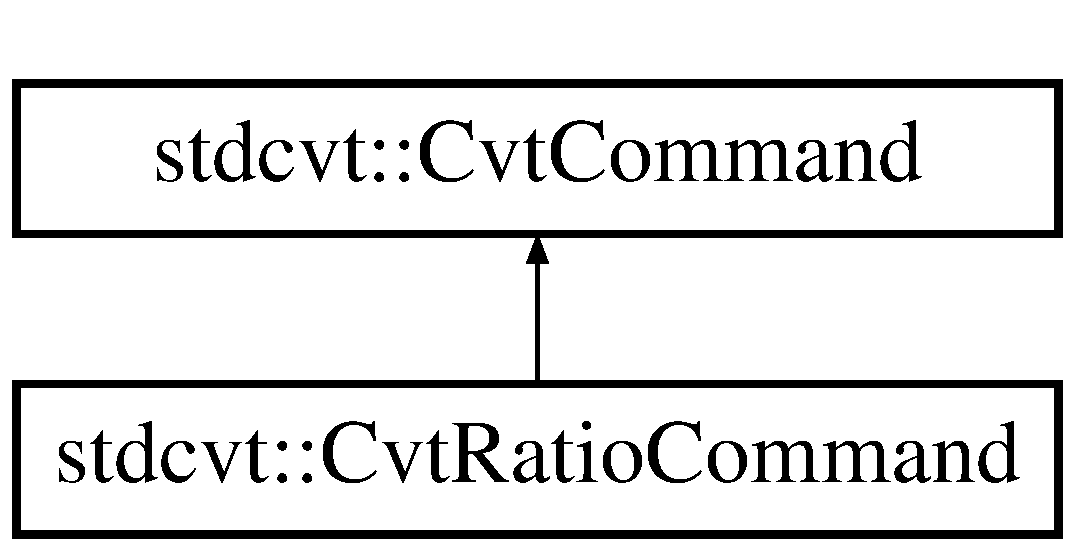
\includegraphics[height=2.000000cm]{classstdcvt_1_1CvtCommand}
\end{center}
\end{figure}
\subsection*{Public 멤버 함수}
\begin{DoxyCompactItemize}
\item 
\hyperlink{classstdcvt_1_1CvtCommand_a8756df160daf11a0cfa7ba6f359120c4}{Cvt\+Command} (int cmdid, \hyperlink{classstdcvt_1_1CvtDeviceSpec}{Cvt\+Device\+Spec} $\ast$pdevspec)
\item 
int \hyperlink{classstdcvt_1_1CvtCommand_a108a615897723b8adaf8d826f1273529}{getid} ()
\item 
bool \hyperlink{classstdcvt_1_1CvtCommand_a6fcd400fd5e627a688a06edcfbcaa210}{getonoff} ()
\item 
bool \hyperlink{classstdcvt_1_1CvtCommand_a933894d3d822018066d4761d56e091f7}{setonoff} (bool onoff)
\end{DoxyCompactItemize}


\subsection{생성자 \& 소멸자 문서화}
\index{stdcvt\+::\+Cvt\+Command@{stdcvt\+::\+Cvt\+Command}!Cvt\+Command@{Cvt\+Command}}
\index{Cvt\+Command@{Cvt\+Command}!stdcvt\+::\+Cvt\+Command@{stdcvt\+::\+Cvt\+Command}}
\subsubsection[{\texorpdfstring{Cvt\+Command(int cmdid, Cvt\+Device\+Spec $\ast$pdevspec)}{CvtCommand(int cmdid, CvtDeviceSpec *pdevspec)}}]{\setlength{\rightskip}{0pt plus 5cm}stdcvt\+::\+Cvt\+Command\+::\+Cvt\+Command (
\begin{DoxyParamCaption}
\item[{int}]{cmdid, }
\item[{{\bf Cvt\+Device\+Spec} $\ast$}]{pdevspec}
\end{DoxyParamCaption}
)\hspace{0.3cm}{\ttfamily [inline]}}\hypertarget{classstdcvt_1_1CvtCommand_a8756df160daf11a0cfa7ba6f359120c4}{}\label{classstdcvt_1_1CvtCommand_a8756df160daf11a0cfa7ba6f359120c4}
새로운 명령를 생성한다. 
\begin{DoxyParams}{매개변수}
{\em cmdid} & 명령의 아이디 \\
\hline
{\em pdev} & 명령을 수행할 장비의 포인터 \\
\hline
\end{DoxyParams}


\subsection{멤버 함수 문서화}
\index{stdcvt\+::\+Cvt\+Command@{stdcvt\+::\+Cvt\+Command}!getid@{getid}}
\index{getid@{getid}!stdcvt\+::\+Cvt\+Command@{stdcvt\+::\+Cvt\+Command}}
\subsubsection[{\texorpdfstring{getid()}{getid()}}]{\setlength{\rightskip}{0pt plus 5cm}int stdcvt\+::\+Cvt\+Command\+::getid (
\begin{DoxyParamCaption}
{}
\end{DoxyParamCaption}
)\hspace{0.3cm}{\ttfamily [inline]}}\hypertarget{classstdcvt_1_1CvtCommand_a108a615897723b8adaf8d826f1273529}{}\label{classstdcvt_1_1CvtCommand_a108a615897723b8adaf8d826f1273529}
명령에 부여된 아이디를 리턴한다. \begin{DoxyReturn}{반환값}
명령의 아이디 
\end{DoxyReturn}
\index{stdcvt\+::\+Cvt\+Command@{stdcvt\+::\+Cvt\+Command}!getonoff@{getonoff}}
\index{getonoff@{getonoff}!stdcvt\+::\+Cvt\+Command@{stdcvt\+::\+Cvt\+Command}}
\subsubsection[{\texorpdfstring{getonoff()}{getonoff()}}]{\setlength{\rightskip}{0pt plus 5cm}bool stdcvt\+::\+Cvt\+Command\+::getonoff (
\begin{DoxyParamCaption}
{}
\end{DoxyParamCaption}
)\hspace{0.3cm}{\ttfamily [inline]}}\hypertarget{classstdcvt_1_1CvtCommand_a6fcd400fd5e627a688a06edcfbcaa210}{}\label{classstdcvt_1_1CvtCommand_a6fcd400fd5e627a688a06edcfbcaa210}
on/off 명령을 확인한다. \begin{DoxyReturn}{반환값}
on이면 true 
\end{DoxyReturn}
\index{stdcvt\+::\+Cvt\+Command@{stdcvt\+::\+Cvt\+Command}!setonoff@{setonoff}}
\index{setonoff@{setonoff}!stdcvt\+::\+Cvt\+Command@{stdcvt\+::\+Cvt\+Command}}
\subsubsection[{\texorpdfstring{setonoff(bool onoff)}{setonoff(bool onoff)}}]{\setlength{\rightskip}{0pt plus 5cm}bool stdcvt\+::\+Cvt\+Command\+::setonoff (
\begin{DoxyParamCaption}
\item[{bool}]{onoff}
\end{DoxyParamCaption}
)\hspace{0.3cm}{\ttfamily [inline]}}\hypertarget{classstdcvt_1_1CvtCommand_a933894d3d822018066d4761d56e091f7}{}\label{classstdcvt_1_1CvtCommand_a933894d3d822018066d4761d56e091f7}
on/off 명령을 세팅한다. 
\begin{DoxyParams}{매개변수}
{\em onoff} & on이면 true \\
\hline
\end{DoxyParams}
\begin{DoxyReturn}{반환값}
세팅된 상태. 
\end{DoxyReturn}


이 클래스에 대한 문서화 페이지는 다음의 파일로부터 생성되었습니다.\+:\begin{DoxyCompactItemize}
\item 
spec/\hyperlink{cvtcommand_8h}{cvtcommand.\+h}\end{DoxyCompactItemize}

\hypertarget{classstdcvt_1_1CvtDevice}{}\section{stdcvt\+:\+:Cvt\+Device 클래스 참조}
\label{classstdcvt_1_1CvtDevice}\index{stdcvt\+::\+Cvt\+Device@{stdcvt\+::\+Cvt\+Device}}
stdcvt\+:\+:Cvt\+Device에 대한 상속 다이어그램 \+: \begin{figure}[H]
\begin{center}
\leavevmode
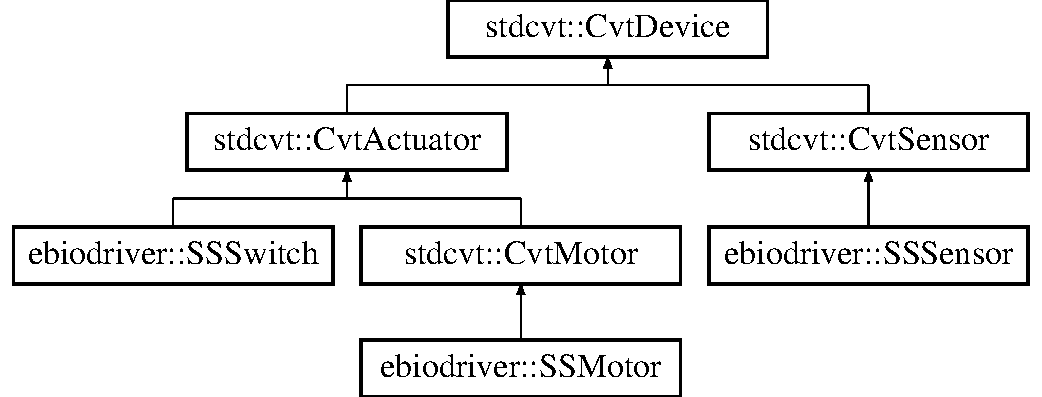
\includegraphics[height=4.000000cm]{classstdcvt_1_1CvtDevice}
\end{center}
\end{figure}
\subsection*{Public 멤버 함수}
\begin{DoxyCompactItemize}
\item 
\hyperlink{classstdcvt_1_1CvtDevice_a551fc68d0c8cbcbc8f6c82b375ea3cb0}{Cvt\+Device} (string devid, \hyperlink{cvtcode_8h_ae8e34073e35cef0bb47c7fa535fc638b}{devtype\+\_\+t} devtype, \hyperlink{cvtcode_8h_a268eebb73363e24b9e65fd51973bd9c0}{devsec\+\_\+t} section, \hyperlink{cvtcode_8h_a2b37fd5cc4d40c0b8c4b987c271e5ceb}{devtarget\+\_\+t} target, \hyperlink{cvtcode_8h_ad21cd565f839adc5b19a0993e7da7278}{devstat\+\_\+t} devstatus)
\item 
string \hyperlink{classstdcvt_1_1CvtDevice_aa575c9dda49790224ccee5f6c4302aaf}{getid} ()
\item 
\hyperlink{classstdcvt_1_1CvtDeviceSpec}{Cvt\+Device\+Spec} $\ast$ \hyperlink{classstdcvt_1_1CvtDevice_a29928ec55be4697cb7ba86268fa6aa8a}{getspec} ()
\item 
\hyperlink{cvtcode_8h_ad21cd565f839adc5b19a0993e7da7278}{devstat\+\_\+t} \hyperlink{classstdcvt_1_1CvtDevice_a87d2288d6211d897e4c2a6c9905f5ff3}{getstatus} ()
\item 
\hyperlink{cvtcode_8h_ad21cd565f839adc5b19a0993e7da7278}{devstat\+\_\+t} \hyperlink{classstdcvt_1_1CvtDevice_a6962f56199cccff1c0687ad5087cb211}{setstatus} (\hyperlink{cvtcode_8h_ad21cd565f839adc5b19a0993e7da7278}{devstat\+\_\+t} devstatus)
\item 
string \hyperlink{classstdcvt_1_1CvtDevice_a93b54587e1940918b825d78b18f48062}{tostring} ()
\end{DoxyCompactItemize}


\subsection{생성자 \& 소멸자 문서화}
\index{stdcvt\+::\+Cvt\+Device@{stdcvt\+::\+Cvt\+Device}!Cvt\+Device@{Cvt\+Device}}
\index{Cvt\+Device@{Cvt\+Device}!stdcvt\+::\+Cvt\+Device@{stdcvt\+::\+Cvt\+Device}}
\subsubsection[{\texorpdfstring{Cvt\+Device(string devid, devtype\+\_\+t devtype, devsec\+\_\+t section, devtarget\+\_\+t target, devstat\+\_\+t devstatus)}{CvtDevice(string devid, devtype_t devtype, devsec_t section, devtarget_t target, devstat_t devstatus)}}]{\setlength{\rightskip}{0pt plus 5cm}stdcvt\+::\+Cvt\+Device\+::\+Cvt\+Device (
\begin{DoxyParamCaption}
\item[{string}]{devid, }
\item[{{\bf devtype\+\_\+t}}]{devtype, }
\item[{{\bf devsec\+\_\+t}}]{section, }
\item[{{\bf devtarget\+\_\+t}}]{target, }
\item[{{\bf devstat\+\_\+t}}]{devstatus}
\end{DoxyParamCaption}
)\hspace{0.3cm}{\ttfamily [inline]}}\hypertarget{classstdcvt_1_1CvtDevice_a551fc68d0c8cbcbc8f6c82b375ea3cb0}{}\label{classstdcvt_1_1CvtDevice_a551fc68d0c8cbcbc8f6c82b375ea3cb0}
새로운 장비를 생성한다. 
\begin{DoxyParams}{매개변수}
{\em devid} & 장비의 아이디 \\
\hline
{\em devtype} & 장비의 종류 \\
\hline
{\em section} & 장비 설치 구역 \\
\hline
{\em target} & 장비의 대상 \\
\hline
{\em devstatus} & 장비의 상태 \\
\hline
\end{DoxyParams}


\subsection{멤버 함수 문서화}
\index{stdcvt\+::\+Cvt\+Device@{stdcvt\+::\+Cvt\+Device}!getid@{getid}}
\index{getid@{getid}!stdcvt\+::\+Cvt\+Device@{stdcvt\+::\+Cvt\+Device}}
\subsubsection[{\texorpdfstring{getid()}{getid()}}]{\setlength{\rightskip}{0pt plus 5cm}string stdcvt\+::\+Cvt\+Device\+::getid (
\begin{DoxyParamCaption}
{}
\end{DoxyParamCaption}
)\hspace{0.3cm}{\ttfamily [inline]}}\hypertarget{classstdcvt_1_1CvtDevice_aa575c9dda49790224ccee5f6c4302aaf}{}\label{classstdcvt_1_1CvtDevice_aa575c9dda49790224ccee5f6c4302aaf}
장비에 부여된 아이디를 리턴한다. \begin{DoxyReturn}{반환값}
장비의 아이디 
\end{DoxyReturn}
\index{stdcvt\+::\+Cvt\+Device@{stdcvt\+::\+Cvt\+Device}!getspec@{getspec}}
\index{getspec@{getspec}!stdcvt\+::\+Cvt\+Device@{stdcvt\+::\+Cvt\+Device}}
\subsubsection[{\texorpdfstring{getspec()}{getspec()}}]{\setlength{\rightskip}{0pt plus 5cm}{\bf Cvt\+Device\+Spec}$\ast$ stdcvt\+::\+Cvt\+Device\+::getspec (
\begin{DoxyParamCaption}
{}
\end{DoxyParamCaption}
)\hspace{0.3cm}{\ttfamily [inline]}}\hypertarget{classstdcvt_1_1CvtDevice_a29928ec55be4697cb7ba86268fa6aa8a}{}\label{classstdcvt_1_1CvtDevice_a29928ec55be4697cb7ba86268fa6aa8a}
장비의 스펙을 리턴한다. \begin{DoxyReturn}{반환값}
장비 스펙의 포인터 
\end{DoxyReturn}
\index{stdcvt\+::\+Cvt\+Device@{stdcvt\+::\+Cvt\+Device}!getstatus@{getstatus}}
\index{getstatus@{getstatus}!stdcvt\+::\+Cvt\+Device@{stdcvt\+::\+Cvt\+Device}}
\subsubsection[{\texorpdfstring{getstatus()}{getstatus()}}]{\setlength{\rightskip}{0pt plus 5cm}{\bf devstat\+\_\+t} stdcvt\+::\+Cvt\+Device\+::getstatus (
\begin{DoxyParamCaption}
{}
\end{DoxyParamCaption}
)\hspace{0.3cm}{\ttfamily [inline]}}\hypertarget{classstdcvt_1_1CvtDevice_a87d2288d6211d897e4c2a6c9905f5ff3}{}\label{classstdcvt_1_1CvtDevice_a87d2288d6211d897e4c2a6c9905f5ff3}
장비의 상태를 리턴한다. \begin{DoxyReturn}{반환값}
장비의 상태 
\end{DoxyReturn}
\index{stdcvt\+::\+Cvt\+Device@{stdcvt\+::\+Cvt\+Device}!setstatus@{setstatus}}
\index{setstatus@{setstatus}!stdcvt\+::\+Cvt\+Device@{stdcvt\+::\+Cvt\+Device}}
\subsubsection[{\texorpdfstring{setstatus(devstat\+\_\+t devstatus)}{setstatus(devstat_t devstatus)}}]{\setlength{\rightskip}{0pt plus 5cm}{\bf devstat\+\_\+t} stdcvt\+::\+Cvt\+Device\+::setstatus (
\begin{DoxyParamCaption}
\item[{{\bf devstat\+\_\+t}}]{devstatus}
\end{DoxyParamCaption}
)\hspace{0.3cm}{\ttfamily [inline]}}\hypertarget{classstdcvt_1_1CvtDevice_a6962f56199cccff1c0687ad5087cb211}{}\label{classstdcvt_1_1CvtDevice_a6962f56199cccff1c0687ad5087cb211}
장비의 상태를 세팅한다. 
\begin{DoxyParams}{매개변수}
{\em devstatus} & 새로 세팅할 장비의 상태 \\
\hline
\end{DoxyParams}
\begin{DoxyReturn}{반환값}
세팅된 장비의 상태 
\end{DoxyReturn}
\index{stdcvt\+::\+Cvt\+Device@{stdcvt\+::\+Cvt\+Device}!tostring@{tostring}}
\index{tostring@{tostring}!stdcvt\+::\+Cvt\+Device@{stdcvt\+::\+Cvt\+Device}}
\subsubsection[{\texorpdfstring{tostring()}{tostring()}}]{\setlength{\rightskip}{0pt plus 5cm}string stdcvt\+::\+Cvt\+Device\+::tostring (
\begin{DoxyParamCaption}
{}
\end{DoxyParamCaption}
)\hspace{0.3cm}{\ttfamily [inline]}}\hypertarget{classstdcvt_1_1CvtDevice_a93b54587e1940918b825d78b18f48062}{}\label{classstdcvt_1_1CvtDevice_a93b54587e1940918b825d78b18f48062}
장비의 상태를 문자열로 내보낸다. 

이 클래스에 대한 문서화 페이지는 다음의 파일로부터 생성되었습니다.\+:\begin{DoxyCompactItemize}
\item 
spec/\hyperlink{cvtdevice_8h}{cvtdevice.\+h}\end{DoxyCompactItemize}

\hypertarget{classstdcvt_1_1CvtDeviceSpec}{}\section{stdcvt\+:\+:Cvt\+Device\+Spec 클래스 참조}
\label{classstdcvt_1_1CvtDeviceSpec}\index{stdcvt\+::\+Cvt\+Device\+Spec@{stdcvt\+::\+Cvt\+Device\+Spec}}
\subsection*{Public 멤버 함수}
\begin{DoxyCompactItemize}
\item 
\hyperlink{classstdcvt_1_1CvtDeviceSpec_aa4e65cb8c2c999a88c8c0af4973a3652}{Cvt\+Device\+Spec} (\hyperlink{cvtcode_8h_ae8e34073e35cef0bb47c7fa535fc638b}{devtype\+\_\+t} devtype, \hyperlink{cvtcode_8h_a268eebb73363e24b9e65fd51973bd9c0}{devsec\+\_\+t} section, \hyperlink{cvtcode_8h_a2b37fd5cc4d40c0b8c4b987c271e5ceb}{devtarget\+\_\+t} target)
\item 
\hyperlink{cvtcode_8h_a2b770a849c30d4f4786dc06b59aef47c}{devgroup\+\_\+t} \hyperlink{classstdcvt_1_1CvtDeviceSpec_a7a122123db7bc9350b89910f8c03b453}{getgrouptype} ()
\item 
\hyperlink{cvtcode_8h_ae8e34073e35cef0bb47c7fa535fc638b}{devtype\+\_\+t} \hyperlink{classstdcvt_1_1CvtDeviceSpec_aebd3553d080f82f7e71d0c145a4e811b}{gettype} ()
\item 
\hyperlink{cvtcode_8h_a268eebb73363e24b9e65fd51973bd9c0}{devsec\+\_\+t} \hyperlink{classstdcvt_1_1CvtDeviceSpec_a1a0224f68343b0ff664492f67b102b02}{getsection} ()
\item 
\hyperlink{cvtcode_8h_a2b37fd5cc4d40c0b8c4b987c271e5ceb}{devtarget\+\_\+t} \hyperlink{classstdcvt_1_1CvtDeviceSpec_acae6e3ba6033ca095b723a541267eab4}{gettarget} ()
\item 
string \hyperlink{classstdcvt_1_1CvtDeviceSpec_a492062d0e23014d77efd75b56d8d21ce}{setmanufacturer} (string manufacturer)
\item 
string \hyperlink{classstdcvt_1_1CvtDeviceSpec_a5aa3ec5557f3a2da7763d13d0da7740c}{getmanufacturer} ()
\item 
string \hyperlink{classstdcvt_1_1CvtDeviceSpec_ad1d1d18f459c2648f325407774f0a44b}{setmodel} (string model)
\item 
string \hyperlink{classstdcvt_1_1CvtDeviceSpec_a9b9a75973c369a9488122848c6a696e8}{getmodel} ()
\item 
bool \hyperlink{classstdcvt_1_1CvtDeviceSpec_a82038a625e1a8705c668ad07a01b5b1f}{copyspec} (\hyperlink{classstdcvt_1_1CvtDeviceSpec}{Cvt\+Device\+Spec} $\ast$pdevspec)
\item 
string \hyperlink{classstdcvt_1_1CvtDeviceSpec_ad3513bc7aad4705052c3ddc4e362294d}{tostring} ()
\item 
bool \hyperlink{classstdcvt_1_1CvtDeviceSpec_a266fe0b00c780140f462586f8b18efce}{checktarget} (\hyperlink{classstdcvt_1_1CvtDeviceSpec}{Cvt\+Device\+Spec} $\ast$pdevspec)
\item 
bool \hyperlink{classstdcvt_1_1CvtDeviceSpec_a631be4b4fa61623932e590c1a2e91c2b}{checktype} (\hyperlink{classstdcvt_1_1CvtDeviceSpec}{Cvt\+Device\+Spec} $\ast$pdevspec)
\item 
bool \hyperlink{classstdcvt_1_1CvtDeviceSpec_a6802ca086da993e02aa224d7c98331ab}{checksection} (\hyperlink{classstdcvt_1_1CvtDeviceSpec}{Cvt\+Device\+Spec} $\ast$pdevspec)
\item 
bool \hyperlink{classstdcvt_1_1CvtDeviceSpec_a88ad24af1eb49a189987576fd1cd231e}{ismatched} (\hyperlink{classstdcvt_1_1CvtDeviceSpec}{Cvt\+Device\+Spec} $\ast$pdevspec)
\end{DoxyCompactItemize}


\subsection{생성자 \& 소멸자 문서화}
\index{stdcvt\+::\+Cvt\+Device\+Spec@{stdcvt\+::\+Cvt\+Device\+Spec}!Cvt\+Device\+Spec@{Cvt\+Device\+Spec}}
\index{Cvt\+Device\+Spec@{Cvt\+Device\+Spec}!stdcvt\+::\+Cvt\+Device\+Spec@{stdcvt\+::\+Cvt\+Device\+Spec}}
\subsubsection[{\texorpdfstring{Cvt\+Device\+Spec(devtype\+\_\+t devtype, devsec\+\_\+t section, devtarget\+\_\+t target)}{CvtDeviceSpec(devtype_t devtype, devsec_t section, devtarget_t target)}}]{\setlength{\rightskip}{0pt plus 5cm}stdcvt\+::\+Cvt\+Device\+Spec\+::\+Cvt\+Device\+Spec (
\begin{DoxyParamCaption}
\item[{{\bf devtype\+\_\+t}}]{devtype, }
\item[{{\bf devsec\+\_\+t}}]{section, }
\item[{{\bf devtarget\+\_\+t}}]{target}
\end{DoxyParamCaption}
)\hspace{0.3cm}{\ttfamily [inline]}}\hypertarget{classstdcvt_1_1CvtDeviceSpec_aa4e65cb8c2c999a88c8c0af4973a3652}{}\label{classstdcvt_1_1CvtDeviceSpec_aa4e65cb8c2c999a88c8c0af4973a3652}
새로운 장비스펙을 생성한다. 
\begin{DoxyParams}{매개변수}
{\em devtype} & 장비의 종류 \\
\hline
{\em section} & 장비 설치 구역 \\
\hline
{\em target} & 장비의 대상 \\
\hline
\end{DoxyParams}


\subsection{멤버 함수 문서화}
\index{stdcvt\+::\+Cvt\+Device\+Spec@{stdcvt\+::\+Cvt\+Device\+Spec}!checksection@{checksection}}
\index{checksection@{checksection}!stdcvt\+::\+Cvt\+Device\+Spec@{stdcvt\+::\+Cvt\+Device\+Spec}}
\subsubsection[{\texorpdfstring{checksection(\+Cvt\+Device\+Spec $\ast$pdevspec)}{checksection(CvtDeviceSpec *pdevspec)}}]{\setlength{\rightskip}{0pt plus 5cm}bool stdcvt\+::\+Cvt\+Device\+Spec\+::checksection (
\begin{DoxyParamCaption}
\item[{{\bf Cvt\+Device\+Spec} $\ast$}]{pdevspec}
\end{DoxyParamCaption}
)\hspace{0.3cm}{\ttfamily [inline]}}\hypertarget{classstdcvt_1_1CvtDeviceSpec_a6802ca086da993e02aa224d7c98331ab}{}\label{classstdcvt_1_1CvtDeviceSpec_a6802ca086da993e02aa224d7c98331ab}
장비설치위치가 매치되는지 확인한다. 
\begin{DoxyParams}{매개변수}
{\em pdevspec} & 확인할 소스 장비스펙에 대한 포인터 \\
\hline
\end{DoxyParams}
\index{stdcvt\+::\+Cvt\+Device\+Spec@{stdcvt\+::\+Cvt\+Device\+Spec}!checktarget@{checktarget}}
\index{checktarget@{checktarget}!stdcvt\+::\+Cvt\+Device\+Spec@{stdcvt\+::\+Cvt\+Device\+Spec}}
\subsubsection[{\texorpdfstring{checktarget(\+Cvt\+Device\+Spec $\ast$pdevspec)}{checktarget(CvtDeviceSpec *pdevspec)}}]{\setlength{\rightskip}{0pt plus 5cm}bool stdcvt\+::\+Cvt\+Device\+Spec\+::checktarget (
\begin{DoxyParamCaption}
\item[{{\bf Cvt\+Device\+Spec} $\ast$}]{pdevspec}
\end{DoxyParamCaption}
)\hspace{0.3cm}{\ttfamily [inline]}}\hypertarget{classstdcvt_1_1CvtDeviceSpec_a266fe0b00c780140f462586f8b18efce}{}\label{classstdcvt_1_1CvtDeviceSpec_a266fe0b00c780140f462586f8b18efce}
장비 작동대상이 매치되는지 확인한다. 
\begin{DoxyParams}{매개변수}
{\em pdevspec} & 확인할 소스 장비스펙에 대한 포인터 \\
\hline
\end{DoxyParams}
\index{stdcvt\+::\+Cvt\+Device\+Spec@{stdcvt\+::\+Cvt\+Device\+Spec}!checktype@{checktype}}
\index{checktype@{checktype}!stdcvt\+::\+Cvt\+Device\+Spec@{stdcvt\+::\+Cvt\+Device\+Spec}}
\subsubsection[{\texorpdfstring{checktype(\+Cvt\+Device\+Spec $\ast$pdevspec)}{checktype(CvtDeviceSpec *pdevspec)}}]{\setlength{\rightskip}{0pt plus 5cm}bool stdcvt\+::\+Cvt\+Device\+Spec\+::checktype (
\begin{DoxyParamCaption}
\item[{{\bf Cvt\+Device\+Spec} $\ast$}]{pdevspec}
\end{DoxyParamCaption}
)\hspace{0.3cm}{\ttfamily [inline]}}\hypertarget{classstdcvt_1_1CvtDeviceSpec_a631be4b4fa61623932e590c1a2e91c2b}{}\label{classstdcvt_1_1CvtDeviceSpec_a631be4b4fa61623932e590c1a2e91c2b}
장비타입이 매치되는지 확인한다. 
\begin{DoxyParams}{매개변수}
{\em pdevspec} & 확인할 소스 장비스펙에 대한 포인터 \\
\hline
\end{DoxyParams}
\index{stdcvt\+::\+Cvt\+Device\+Spec@{stdcvt\+::\+Cvt\+Device\+Spec}!copyspec@{copyspec}}
\index{copyspec@{copyspec}!stdcvt\+::\+Cvt\+Device\+Spec@{stdcvt\+::\+Cvt\+Device\+Spec}}
\subsubsection[{\texorpdfstring{copyspec(\+Cvt\+Device\+Spec $\ast$pdevspec)}{copyspec(CvtDeviceSpec *pdevspec)}}]{\setlength{\rightskip}{0pt plus 5cm}bool stdcvt\+::\+Cvt\+Device\+Spec\+::copyspec (
\begin{DoxyParamCaption}
\item[{{\bf Cvt\+Device\+Spec} $\ast$}]{pdevspec}
\end{DoxyParamCaption}
)\hspace{0.3cm}{\ttfamily [inline]}}\hypertarget{classstdcvt_1_1CvtDeviceSpec_a82038a625e1a8705c668ad07a01b5b1f}{}\label{classstdcvt_1_1CvtDeviceSpec_a82038a625e1a8705c668ad07a01b5b1f}
장비의 속성을 복사한다. 
\begin{DoxyParams}{매개변수}
{\em pdevspec} & 복사할 소스 장비스펙에 대한 포인터 \\
\hline
\end{DoxyParams}
\index{stdcvt\+::\+Cvt\+Device\+Spec@{stdcvt\+::\+Cvt\+Device\+Spec}!getgrouptype@{getgrouptype}}
\index{getgrouptype@{getgrouptype}!stdcvt\+::\+Cvt\+Device\+Spec@{stdcvt\+::\+Cvt\+Device\+Spec}}
\subsubsection[{\texorpdfstring{getgrouptype()}{getgrouptype()}}]{\setlength{\rightskip}{0pt plus 5cm}{\bf devgroup\+\_\+t} stdcvt\+::\+Cvt\+Device\+Spec\+::getgrouptype (
\begin{DoxyParamCaption}
{}
\end{DoxyParamCaption}
)\hspace{0.3cm}{\ttfamily [inline]}}\hypertarget{classstdcvt_1_1CvtDeviceSpec_a7a122123db7bc9350b89910f8c03b453}{}\label{classstdcvt_1_1CvtDeviceSpec_a7a122123db7bc9350b89910f8c03b453}
장비그룹의 종류를 리턴한다. \begin{DoxyReturn}{반환값}
장비그룹의 종류 
\end{DoxyReturn}
\index{stdcvt\+::\+Cvt\+Device\+Spec@{stdcvt\+::\+Cvt\+Device\+Spec}!getmanufacturer@{getmanufacturer}}
\index{getmanufacturer@{getmanufacturer}!stdcvt\+::\+Cvt\+Device\+Spec@{stdcvt\+::\+Cvt\+Device\+Spec}}
\subsubsection[{\texorpdfstring{getmanufacturer()}{getmanufacturer()}}]{\setlength{\rightskip}{0pt plus 5cm}string stdcvt\+::\+Cvt\+Device\+Spec\+::getmanufacturer (
\begin{DoxyParamCaption}
{}
\end{DoxyParamCaption}
)\hspace{0.3cm}{\ttfamily [inline]}}\hypertarget{classstdcvt_1_1CvtDeviceSpec_a5aa3ec5557f3a2da7763d13d0da7740c}{}\label{classstdcvt_1_1CvtDeviceSpec_a5aa3ec5557f3a2da7763d13d0da7740c}
장비의 제조사를 확인한다. \begin{DoxyReturn}{반환값}
세팅된 장비 제조사 
\end{DoxyReturn}
\index{stdcvt\+::\+Cvt\+Device\+Spec@{stdcvt\+::\+Cvt\+Device\+Spec}!getmodel@{getmodel}}
\index{getmodel@{getmodel}!stdcvt\+::\+Cvt\+Device\+Spec@{stdcvt\+::\+Cvt\+Device\+Spec}}
\subsubsection[{\texorpdfstring{getmodel()}{getmodel()}}]{\setlength{\rightskip}{0pt plus 5cm}string stdcvt\+::\+Cvt\+Device\+Spec\+::getmodel (
\begin{DoxyParamCaption}
{}
\end{DoxyParamCaption}
)\hspace{0.3cm}{\ttfamily [inline]}}\hypertarget{classstdcvt_1_1CvtDeviceSpec_a9b9a75973c369a9488122848c6a696e8}{}\label{classstdcvt_1_1CvtDeviceSpec_a9b9a75973c369a9488122848c6a696e8}
장비의 모델을 확인한다. \begin{DoxyReturn}{반환값}
세팅된 장비 모델 
\end{DoxyReturn}
\index{stdcvt\+::\+Cvt\+Device\+Spec@{stdcvt\+::\+Cvt\+Device\+Spec}!getsection@{getsection}}
\index{getsection@{getsection}!stdcvt\+::\+Cvt\+Device\+Spec@{stdcvt\+::\+Cvt\+Device\+Spec}}
\subsubsection[{\texorpdfstring{getsection()}{getsection()}}]{\setlength{\rightskip}{0pt plus 5cm}{\bf devsec\+\_\+t} stdcvt\+::\+Cvt\+Device\+Spec\+::getsection (
\begin{DoxyParamCaption}
{}
\end{DoxyParamCaption}
)\hspace{0.3cm}{\ttfamily [inline]}}\hypertarget{classstdcvt_1_1CvtDeviceSpec_a1a0224f68343b0ff664492f67b102b02}{}\label{classstdcvt_1_1CvtDeviceSpec_a1a0224f68343b0ff664492f67b102b02}
장비의 설치구역을 리턴한다. \begin{DoxyReturn}{반환값}
장비의 설치구역 
\end{DoxyReturn}
\index{stdcvt\+::\+Cvt\+Device\+Spec@{stdcvt\+::\+Cvt\+Device\+Spec}!gettarget@{gettarget}}
\index{gettarget@{gettarget}!stdcvt\+::\+Cvt\+Device\+Spec@{stdcvt\+::\+Cvt\+Device\+Spec}}
\subsubsection[{\texorpdfstring{gettarget()}{gettarget()}}]{\setlength{\rightskip}{0pt plus 5cm}{\bf devtarget\+\_\+t} stdcvt\+::\+Cvt\+Device\+Spec\+::gettarget (
\begin{DoxyParamCaption}
{}
\end{DoxyParamCaption}
)\hspace{0.3cm}{\ttfamily [inline]}}\hypertarget{classstdcvt_1_1CvtDeviceSpec_acae6e3ba6033ca095b723a541267eab4}{}\label{classstdcvt_1_1CvtDeviceSpec_acae6e3ba6033ca095b723a541267eab4}
장비의 대상을 리턴한다. \begin{DoxyReturn}{반환값}
장비의 대상 
\end{DoxyReturn}
\index{stdcvt\+::\+Cvt\+Device\+Spec@{stdcvt\+::\+Cvt\+Device\+Spec}!gettype@{gettype}}
\index{gettype@{gettype}!stdcvt\+::\+Cvt\+Device\+Spec@{stdcvt\+::\+Cvt\+Device\+Spec}}
\subsubsection[{\texorpdfstring{gettype()}{gettype()}}]{\setlength{\rightskip}{0pt plus 5cm}{\bf devtype\+\_\+t} stdcvt\+::\+Cvt\+Device\+Spec\+::gettype (
\begin{DoxyParamCaption}
{}
\end{DoxyParamCaption}
)\hspace{0.3cm}{\ttfamily [inline]}}\hypertarget{classstdcvt_1_1CvtDeviceSpec_aebd3553d080f82f7e71d0c145a4e811b}{}\label{classstdcvt_1_1CvtDeviceSpec_aebd3553d080f82f7e71d0c145a4e811b}
장비의 종류를 리턴한다. \begin{DoxyReturn}{반환값}
장비의 종류 
\end{DoxyReturn}
\index{stdcvt\+::\+Cvt\+Device\+Spec@{stdcvt\+::\+Cvt\+Device\+Spec}!ismatched@{ismatched}}
\index{ismatched@{ismatched}!stdcvt\+::\+Cvt\+Device\+Spec@{stdcvt\+::\+Cvt\+Device\+Spec}}
\subsubsection[{\texorpdfstring{ismatched(\+Cvt\+Device\+Spec $\ast$pdevspec)}{ismatched(CvtDeviceSpec *pdevspec)}}]{\setlength{\rightskip}{0pt plus 5cm}bool stdcvt\+::\+Cvt\+Device\+Spec\+::ismatched (
\begin{DoxyParamCaption}
\item[{{\bf Cvt\+Device\+Spec} $\ast$}]{pdevspec}
\end{DoxyParamCaption}
)\hspace{0.3cm}{\ttfamily [inline]}}\hypertarget{classstdcvt_1_1CvtDeviceSpec_a88ad24af1eb49a189987576fd1cd231e}{}\label{classstdcvt_1_1CvtDeviceSpec_a88ad24af1eb49a189987576fd1cd231e}
장비스펙이 매치되는지 확인한다. 
\begin{DoxyParams}{매개변수}
{\em pdevspec} & 확인할 소스 장비스펙에 대한 포인터 \\
\hline
\end{DoxyParams}
\index{stdcvt\+::\+Cvt\+Device\+Spec@{stdcvt\+::\+Cvt\+Device\+Spec}!setmanufacturer@{setmanufacturer}}
\index{setmanufacturer@{setmanufacturer}!stdcvt\+::\+Cvt\+Device\+Spec@{stdcvt\+::\+Cvt\+Device\+Spec}}
\subsubsection[{\texorpdfstring{setmanufacturer(string manufacturer)}{setmanufacturer(string manufacturer)}}]{\setlength{\rightskip}{0pt plus 5cm}string stdcvt\+::\+Cvt\+Device\+Spec\+::setmanufacturer (
\begin{DoxyParamCaption}
\item[{string}]{manufacturer}
\end{DoxyParamCaption}
)\hspace{0.3cm}{\ttfamily [inline]}}\hypertarget{classstdcvt_1_1CvtDeviceSpec_a492062d0e23014d77efd75b56d8d21ce}{}\label{classstdcvt_1_1CvtDeviceSpec_a492062d0e23014d77efd75b56d8d21ce}
장비의 제조사를 세팅한다. 
\begin{DoxyParams}{매개변수}
{\em manufacturer} & 장비 제조사 \\
\hline
\end{DoxyParams}
\begin{DoxyReturn}{반환값}
세팅된 장비 제조사 
\end{DoxyReturn}
\index{stdcvt\+::\+Cvt\+Device\+Spec@{stdcvt\+::\+Cvt\+Device\+Spec}!setmodel@{setmodel}}
\index{setmodel@{setmodel}!stdcvt\+::\+Cvt\+Device\+Spec@{stdcvt\+::\+Cvt\+Device\+Spec}}
\subsubsection[{\texorpdfstring{setmodel(string model)}{setmodel(string model)}}]{\setlength{\rightskip}{0pt plus 5cm}string stdcvt\+::\+Cvt\+Device\+Spec\+::setmodel (
\begin{DoxyParamCaption}
\item[{string}]{model}
\end{DoxyParamCaption}
)\hspace{0.3cm}{\ttfamily [inline]}}\hypertarget{classstdcvt_1_1CvtDeviceSpec_ad1d1d18f459c2648f325407774f0a44b}{}\label{classstdcvt_1_1CvtDeviceSpec_ad1d1d18f459c2648f325407774f0a44b}
장비의 모델을 세팅한다. 
\begin{DoxyParams}{매개변수}
{\em model} & 장비 모델 \\
\hline
\end{DoxyParams}
\begin{DoxyReturn}{반환값}
세팅된 장비 모델 
\end{DoxyReturn}
\index{stdcvt\+::\+Cvt\+Device\+Spec@{stdcvt\+::\+Cvt\+Device\+Spec}!tostring@{tostring}}
\index{tostring@{tostring}!stdcvt\+::\+Cvt\+Device\+Spec@{stdcvt\+::\+Cvt\+Device\+Spec}}
\subsubsection[{\texorpdfstring{tostring()}{tostring()}}]{\setlength{\rightskip}{0pt plus 5cm}string stdcvt\+::\+Cvt\+Device\+Spec\+::tostring (
\begin{DoxyParamCaption}
{}
\end{DoxyParamCaption}
)\hspace{0.3cm}{\ttfamily [inline]}}\hypertarget{classstdcvt_1_1CvtDeviceSpec_ad3513bc7aad4705052c3ddc4e362294d}{}\label{classstdcvt_1_1CvtDeviceSpec_ad3513bc7aad4705052c3ddc4e362294d}
장비의 스펙을 문자열로 내보낸다. 

이 클래스에 대한 문서화 페이지는 다음의 파일로부터 생성되었습니다.\+:\begin{DoxyCompactItemize}
\item 
spec/\hyperlink{cvtdevicespec_8h}{cvtdevicespec.\+h}\end{DoxyCompactItemize}

\hypertarget{classstdcvt_1_1CvtDriver}{}\section{stdcvt\+:\+:Cvt\+Driver 클래스 참조}
\label{classstdcvt_1_1CvtDriver}\index{stdcvt\+::\+Cvt\+Driver@{stdcvt\+::\+Cvt\+Driver}}
stdcvt\+:\+:Cvt\+Driver에 대한 상속 다이어그램 \+: \begin{figure}[H]
\begin{center}
\leavevmode
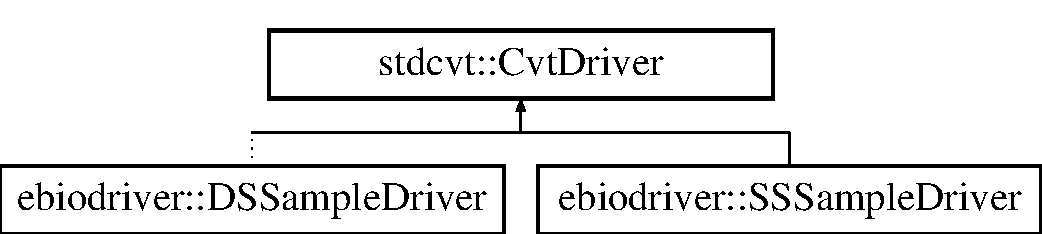
\includegraphics[height=2.000000cm]{classstdcvt_1_1CvtDriver}
\end{center}
\end{figure}
\subsection*{Public 멤버 함수}
\begin{DoxyCompactItemize}
\item 
\hyperlink{classstdcvt_1_1CvtDriver_a82925971b6e8ef2ce7f0b5d113120855}{Cvt\+Driver} (int modelcode, int apispec)
\item 
int \hyperlink{classstdcvt_1_1CvtDriver_a86ffa63425176824f6b0493be4e41cda}{getmodelcode} ()
\item 
int \hyperlink{classstdcvt_1_1CvtDriver_ad6e0edc0bc47015d446215e98b7bfc2f}{getapispec} ()
\item 
virtual const char $\ast$ \hyperlink{classstdcvt_1_1CvtDriver_a8c813cb2be4b0f3bb02c99125488ac24}{getversion} ()=0
\item 
virtual const char $\ast$ \hyperlink{classstdcvt_1_1CvtDriver_a384233eb993e566102cbcc5e87db3e96}{getmodel} ()=0
\item 
virtual const char $\ast$ \hyperlink{classstdcvt_1_1CvtDriver_af77365bd31120078fa2eae4ddece3028}{getcompany} ()=0
\item 
virtual bool \hyperlink{classstdcvt_1_1CvtDriver_a71322934c5b5ad0d5b167219cd23a0bb}{initialize} (\hyperlink{classstdcvt_1_1CvtOption}{Cvt\+Option} option)=0
\item 
virtual bool \hyperlink{classstdcvt_1_1CvtDriver_a22b39da5aafabec2ee9677ed138256e9}{finalize} ()=0
\item 
virtual bool \hyperlink{classstdcvt_1_1CvtDriver_ac15259a26d652d46c198307886d52257}{preprocess} ()=0
\item 
virtual bool \hyperlink{classstdcvt_1_1CvtDriver_a4bcae9e7c58d989a645a74d21e2fc5ea}{postprocess} ()=0
\item 
virtual \hyperlink{classstdcvt_1_1CvtDevice}{Cvt\+Device} $\ast$ \hyperlink{classstdcvt_1_1CvtDriver_adc2ce5ff6fe2426fd84ce3ae69731704}{getdevice} (int index)=0
\item 
virtual bool \hyperlink{classstdcvt_1_1CvtDriver_aeedcd62d3b6ed95f0584db5a7259f642}{sharedevice} (\hyperlink{classstdcvt_1_1CvtDevice}{Cvt\+Device} $\ast$pdevice)=0
\item 
virtual \hyperlink{classstdcvt_1_1CvtCommand}{Cvt\+Command} $\ast$ \hyperlink{classstdcvt_1_1CvtDriver_ad0378635152f2e35c0686c4fe92996e6}{getcommand} (int index)=0
\item 
virtual bool \hyperlink{classstdcvt_1_1CvtDriver_ac289321a67d660f5514c4ddfaa238ade}{control} (\hyperlink{classstdcvt_1_1CvtCommand}{Cvt\+Command} $\ast$pcmd)=0
\end{DoxyCompactItemize}


\subsection{생성자 \& 소멸자 문서화}
\index{stdcvt\+::\+Cvt\+Driver@{stdcvt\+::\+Cvt\+Driver}!Cvt\+Driver@{Cvt\+Driver}}
\index{Cvt\+Driver@{Cvt\+Driver}!stdcvt\+::\+Cvt\+Driver@{stdcvt\+::\+Cvt\+Driver}}
\subsubsection[{\texorpdfstring{Cvt\+Driver(int modelcode, int apispec)}{CvtDriver(int modelcode, int apispec)}}]{\setlength{\rightskip}{0pt plus 5cm}stdcvt\+::\+Cvt\+Driver\+::\+Cvt\+Driver (
\begin{DoxyParamCaption}
\item[{int}]{modelcode, }
\item[{int}]{apispec}
\end{DoxyParamCaption}
)\hspace{0.3cm}{\ttfamily [inline]}}\hypertarget{classstdcvt_1_1CvtDriver_a82925971b6e8ef2ce7f0b5d113120855}{}\label{classstdcvt_1_1CvtDriver_a82925971b6e8ef2ce7f0b5d113120855}
새로운 드라이버를 생성한다. 
\begin{DoxyParams}{매개변수}
{\em modelcode} & 모델코드 \\
\hline
{\em apispec} & A\+PI 버전 \\
\hline
\end{DoxyParams}


\subsection{멤버 함수 문서화}
\index{stdcvt\+::\+Cvt\+Driver@{stdcvt\+::\+Cvt\+Driver}!control@{control}}
\index{control@{control}!stdcvt\+::\+Cvt\+Driver@{stdcvt\+::\+Cvt\+Driver}}
\subsubsection[{\texorpdfstring{control(\+Cvt\+Command $\ast$pcmd)=0}{control(CvtCommand *pcmd)=0}}]{\setlength{\rightskip}{0pt plus 5cm}virtual bool stdcvt\+::\+Cvt\+Driver\+::control (
\begin{DoxyParamCaption}
\item[{{\bf Cvt\+Command} $\ast$}]{pcmd}
\end{DoxyParamCaption}
)\hspace{0.3cm}{\ttfamily [pure virtual]}}\hypertarget{classstdcvt_1_1CvtDriver_ac289321a67d660f5514c4ddfaa238ade}{}\label{classstdcvt_1_1CvtDriver_ac289321a67d660f5514c4ddfaa238ade}
다른 드라이버로부터 명령을 받아 처리한다. 
\begin{DoxyParams}{매개변수}
{\em pcmd} & 명령에 대한 포인터 \\
\hline
\end{DoxyParams}
\begin{DoxyReturn}{반환값}
실제 명령의 처리 여부가 아니라 명령을 수신했는지 여부이다. 해당 명령을 실행할 장비가 없다면 false이다. 
\end{DoxyReturn}


\hyperlink{classebiodriver_1_1DSSampleDriver_a0fe50dbf8dd10f4568f25e83e7e3e873}{ebiodriver\+::\+D\+S\+Sample\+Driver}, \hyperlink{classebiodriver_1_1SSSampleDriver_a25e63484cfbe11d3bc741c1cad5b240c}{ebiodriver\+::\+S\+S\+Sample\+Driver}에서 구현되었습니다.

\index{stdcvt\+::\+Cvt\+Driver@{stdcvt\+::\+Cvt\+Driver}!finalize@{finalize}}
\index{finalize@{finalize}!stdcvt\+::\+Cvt\+Driver@{stdcvt\+::\+Cvt\+Driver}}
\subsubsection[{\texorpdfstring{finalize()=0}{finalize()=0}}]{\setlength{\rightskip}{0pt plus 5cm}virtual bool stdcvt\+::\+Cvt\+Driver\+::finalize (
\begin{DoxyParamCaption}
{}
\end{DoxyParamCaption}
)\hspace{0.3cm}{\ttfamily [pure virtual]}}\hypertarget{classstdcvt_1_1CvtDriver_a22b39da5aafabec2ee9677ed138256e9}{}\label{classstdcvt_1_1CvtDriver_a22b39da5aafabec2ee9677ed138256e9}
드라이버를 종료한다. \begin{DoxyReturn}{반환값}
종료 성공 여부 
\end{DoxyReturn}


\hyperlink{classebiodriver_1_1DSSampleDriver_a21e12d56a042bc9efee56f9af7e41f7c}{ebiodriver\+::\+D\+S\+Sample\+Driver}, \hyperlink{classebiodriver_1_1SSSampleDriver_a43ab28051c128755cbb639d1c2db7ab2}{ebiodriver\+::\+S\+S\+Sample\+Driver}에서 구현되었습니다.

\index{stdcvt\+::\+Cvt\+Driver@{stdcvt\+::\+Cvt\+Driver}!getapispec@{getapispec}}
\index{getapispec@{getapispec}!stdcvt\+::\+Cvt\+Driver@{stdcvt\+::\+Cvt\+Driver}}
\subsubsection[{\texorpdfstring{getapispec()}{getapispec()}}]{\setlength{\rightskip}{0pt plus 5cm}int stdcvt\+::\+Cvt\+Driver\+::getapispec (
\begin{DoxyParamCaption}
{}
\end{DoxyParamCaption}
)\hspace{0.3cm}{\ttfamily [inline]}}\hypertarget{classstdcvt_1_1CvtDriver_ad6e0edc0bc47015d446215e98b7bfc2f}{}\label{classstdcvt_1_1CvtDriver_ad6e0edc0bc47015d446215e98b7bfc2f}
드라이버의 A\+PI 버전을 확인한다. \begin{DoxyReturn}{반환값}
드라이버의 A\+PI 버전 
\end{DoxyReturn}
\index{stdcvt\+::\+Cvt\+Driver@{stdcvt\+::\+Cvt\+Driver}!getcommand@{getcommand}}
\index{getcommand@{getcommand}!stdcvt\+::\+Cvt\+Driver@{stdcvt\+::\+Cvt\+Driver}}
\subsubsection[{\texorpdfstring{getcommand(int index)=0}{getcommand(int index)=0}}]{\setlength{\rightskip}{0pt plus 5cm}virtual {\bf Cvt\+Command}$\ast$ stdcvt\+::\+Cvt\+Driver\+::getcommand (
\begin{DoxyParamCaption}
\item[{int}]{index}
\end{DoxyParamCaption}
)\hspace{0.3cm}{\ttfamily [pure virtual]}}\hypertarget{classstdcvt_1_1CvtDriver_ad0378635152f2e35c0686c4fe92996e6}{}\label{classstdcvt_1_1CvtDriver_ad0378635152f2e35c0686c4fe92996e6}
다른 드라이버가 관리하고 있는 장비를 제어하고자 할때 명령을 전달한다. 명령을 전달하지 않는 드라이버라면 그냥 N\+U\+L\+L을 리턴하도록 만들면 된다. 
\begin{DoxyParams}{매개변수}
{\em index} & 얻고자 하는 명령의 인덱스 번호. 0에서 시작한다. \\
\hline
\end{DoxyParams}
\begin{DoxyReturn}{반환값}
인덱스에 해당하는 명령의 포인터. N\+U\+LL 이라면 이후에 명령이 없다는 의미이다. 
\end{DoxyReturn}


\hyperlink{classebiodriver_1_1DSSampleDriver_acfccb95870864ce6dc5f99ab94c214fa}{ebiodriver\+::\+D\+S\+Sample\+Driver}, \hyperlink{classebiodriver_1_1SSSampleDriver_a273a5a2d7a1b54ba4d6d3989db78d152}{ebiodriver\+::\+S\+S\+Sample\+Driver}에서 구현되었습니다.

\index{stdcvt\+::\+Cvt\+Driver@{stdcvt\+::\+Cvt\+Driver}!getcompany@{getcompany}}
\index{getcompany@{getcompany}!stdcvt\+::\+Cvt\+Driver@{stdcvt\+::\+Cvt\+Driver}}
\subsubsection[{\texorpdfstring{getcompany()=0}{getcompany()=0}}]{\setlength{\rightskip}{0pt plus 5cm}virtual const char$\ast$ stdcvt\+::\+Cvt\+Driver\+::getcompany (
\begin{DoxyParamCaption}
{}
\end{DoxyParamCaption}
)\hspace{0.3cm}{\ttfamily [pure virtual]}}\hypertarget{classstdcvt_1_1CvtDriver_af77365bd31120078fa2eae4ddece3028}{}\label{classstdcvt_1_1CvtDriver_af77365bd31120078fa2eae4ddece3028}
드라이버 제조사명을 확인한다. 컨버터에서는 제조사명을 로깅용도로만 사용한다. \begin{DoxyReturn}{반환값}
문자열 형식의 제조사명 
\end{DoxyReturn}


\hyperlink{classebiodriver_1_1DSSampleDriver_aa0f1649252e066e3543ee962b09521e5}{ebiodriver\+::\+D\+S\+Sample\+Driver}, \hyperlink{classebiodriver_1_1SSSampleDriver_a34f317b0b97ad61cb6b9efe0f1920e21}{ebiodriver\+::\+S\+S\+Sample\+Driver}에서 구현되었습니다.

\index{stdcvt\+::\+Cvt\+Driver@{stdcvt\+::\+Cvt\+Driver}!getdevice@{getdevice}}
\index{getdevice@{getdevice}!stdcvt\+::\+Cvt\+Driver@{stdcvt\+::\+Cvt\+Driver}}
\subsubsection[{\texorpdfstring{getdevice(int index)=0}{getdevice(int index)=0}}]{\setlength{\rightskip}{0pt plus 5cm}virtual {\bf Cvt\+Device}$\ast$ stdcvt\+::\+Cvt\+Driver\+::getdevice (
\begin{DoxyParamCaption}
\item[{int}]{index}
\end{DoxyParamCaption}
)\hspace{0.3cm}{\ttfamily [pure virtual]}}\hypertarget{classstdcvt_1_1CvtDriver_adc2ce5ff6fe2426fd84ce3ae69731704}{}\label{classstdcvt_1_1CvtDriver_adc2ce5ff6fe2426fd84ce3ae69731704}
드라이버가 관리하고 있는 장비의 포인터를 꺼내준다. 모든 장비를 꺼내주지않고, 변경된 장비만을 꺼내주는 방식으로 효율을 높일 수 있다. 
\begin{DoxyParams}{매개변수}
{\em index} & 얻고자 하는 장비의 인덱스 번호. 0에서 시작한다. \\
\hline
\end{DoxyParams}
\begin{DoxyReturn}{반환값}
인덱스에 해당하는 장비의 포인터. N\+U\+LL 이라면 이후에 장비가 없다는 의미이다. 
\end{DoxyReturn}


\hyperlink{classebiodriver_1_1DSSampleDriver_a3dcd13870509c3139c6c0ad7ba22cbed}{ebiodriver\+::\+D\+S\+Sample\+Driver}, \hyperlink{classebiodriver_1_1SSSampleDriver_af4bdb5522559606b177416ec408cd4b4}{ebiodriver\+::\+S\+S\+Sample\+Driver}에서 구현되었습니다.

\index{stdcvt\+::\+Cvt\+Driver@{stdcvt\+::\+Cvt\+Driver}!getmodel@{getmodel}}
\index{getmodel@{getmodel}!stdcvt\+::\+Cvt\+Driver@{stdcvt\+::\+Cvt\+Driver}}
\subsubsection[{\texorpdfstring{getmodel()=0}{getmodel()=0}}]{\setlength{\rightskip}{0pt plus 5cm}virtual const char$\ast$ stdcvt\+::\+Cvt\+Driver\+::getmodel (
\begin{DoxyParamCaption}
{}
\end{DoxyParamCaption}
)\hspace{0.3cm}{\ttfamily [pure virtual]}}\hypertarget{classstdcvt_1_1CvtDriver_a384233eb993e566102cbcc5e87db3e96}{}\label{classstdcvt_1_1CvtDriver_a384233eb993e566102cbcc5e87db3e96}
드라이버 제작자가 부여하는 모델번호를 확인한다. 컨버터에서는 모델코드만 확인하고, 모델번호에 대해서는 로깅용도로만 사용한다. \begin{DoxyReturn}{반환값}
문자열 형식의 모델번호 
\end{DoxyReturn}


\hyperlink{classebiodriver_1_1DSSampleDriver_adf31d39b45faa75dec37919861c99d9d}{ebiodriver\+::\+D\+S\+Sample\+Driver}, \hyperlink{classebiodriver_1_1SSSampleDriver_ac901fe0974866f1fa494b0bad342c562}{ebiodriver\+::\+S\+S\+Sample\+Driver}에서 구현되었습니다.

\index{stdcvt\+::\+Cvt\+Driver@{stdcvt\+::\+Cvt\+Driver}!getmodelcode@{getmodelcode}}
\index{getmodelcode@{getmodelcode}!stdcvt\+::\+Cvt\+Driver@{stdcvt\+::\+Cvt\+Driver}}
\subsubsection[{\texorpdfstring{getmodelcode()}{getmodelcode()}}]{\setlength{\rightskip}{0pt plus 5cm}int stdcvt\+::\+Cvt\+Driver\+::getmodelcode (
\begin{DoxyParamCaption}
{}
\end{DoxyParamCaption}
)\hspace{0.3cm}{\ttfamily [inline]}}\hypertarget{classstdcvt_1_1CvtDriver_a86ffa63425176824f6b0493be4e41cda}{}\label{classstdcvt_1_1CvtDriver_a86ffa63425176824f6b0493be4e41cda}
드라이버의 모델코드를 확인한다. \begin{DoxyReturn}{반환값}
드라이버의 모델코드 
\end{DoxyReturn}
\index{stdcvt\+::\+Cvt\+Driver@{stdcvt\+::\+Cvt\+Driver}!getversion@{getversion}}
\index{getversion@{getversion}!stdcvt\+::\+Cvt\+Driver@{stdcvt\+::\+Cvt\+Driver}}
\subsubsection[{\texorpdfstring{getversion()=0}{getversion()=0}}]{\setlength{\rightskip}{0pt plus 5cm}virtual const char$\ast$ stdcvt\+::\+Cvt\+Driver\+::getversion (
\begin{DoxyParamCaption}
{}
\end{DoxyParamCaption}
)\hspace{0.3cm}{\ttfamily [pure virtual]}}\hypertarget{classstdcvt_1_1CvtDriver_a8c813cb2be4b0f3bb02c99125488ac24}{}\label{classstdcvt_1_1CvtDriver_a8c813cb2be4b0f3bb02c99125488ac24}
드라이버 제작자가 부여하는 버전번호를 확인한다. 컨버터에서는 해당 버전을 로깅용도로만 사용한다. 문자열 비교를 통해 후순위가 더 높은 버전이 된다. \begin{DoxyReturn}{반환값}
문자열 형식의 버전번호 
\end{DoxyReturn}


\hyperlink{classebiodriver_1_1DSSampleDriver_a0ce406b8c18871ab2ac506d5137543c1}{ebiodriver\+::\+D\+S\+Sample\+Driver}, \hyperlink{classebiodriver_1_1SSSampleDriver_a63d048b6c45e48bfc8f27e6a000a17fb}{ebiodriver\+::\+S\+S\+Sample\+Driver}에서 구현되었습니다.

\index{stdcvt\+::\+Cvt\+Driver@{stdcvt\+::\+Cvt\+Driver}!initialize@{initialize}}
\index{initialize@{initialize}!stdcvt\+::\+Cvt\+Driver@{stdcvt\+::\+Cvt\+Driver}}
\subsubsection[{\texorpdfstring{initialize(\+Cvt\+Option option)=0}{initialize(CvtOption option)=0}}]{\setlength{\rightskip}{0pt plus 5cm}virtual bool stdcvt\+::\+Cvt\+Driver\+::initialize (
\begin{DoxyParamCaption}
\item[{{\bf Cvt\+Option}}]{option}
\end{DoxyParamCaption}
)\hspace{0.3cm}{\ttfamily [pure virtual]}}\hypertarget{classstdcvt_1_1CvtDriver_a71322934c5b5ad0d5b167219cd23a0bb}{}\label{classstdcvt_1_1CvtDriver_a71322934c5b5ad0d5b167219cd23a0bb}
드라이버를 초기화 한다. 드라이버 동작을 위한 option 은 key-\/value 형식으로 전달된다. 
\begin{DoxyParams}{매개변수}
{\em option} & 드라이버동작을 위한 옵션 \\
\hline
\end{DoxyParams}
\begin{DoxyReturn}{반환값}
초기화 성공 여부 
\end{DoxyReturn}


\hyperlink{classebiodriver_1_1DSSampleDriver_aaeb74b5cfe475ecdafe87279574fe6e4}{ebiodriver\+::\+D\+S\+Sample\+Driver}, \hyperlink{classebiodriver_1_1SSSampleDriver_a604f906153e106692bd5869c7fd8888f}{ebiodriver\+::\+S\+S\+Sample\+Driver}에서 구현되었습니다.

\index{stdcvt\+::\+Cvt\+Driver@{stdcvt\+::\+Cvt\+Driver}!postprocess@{postprocess}}
\index{postprocess@{postprocess}!stdcvt\+::\+Cvt\+Driver@{stdcvt\+::\+Cvt\+Driver}}
\subsubsection[{\texorpdfstring{postprocess()=0}{postprocess()=0}}]{\setlength{\rightskip}{0pt plus 5cm}virtual bool stdcvt\+::\+Cvt\+Driver\+::postprocess (
\begin{DoxyParamCaption}
{}
\end{DoxyParamCaption}
)\hspace{0.3cm}{\ttfamily [pure virtual]}}\hypertarget{classstdcvt_1_1CvtDriver_a4bcae9e7c58d989a645a74d21e2fc5ea}{}\label{classstdcvt_1_1CvtDriver_a4bcae9e7c58d989a645a74d21e2fc5ea}
드라이버간 상태교환이 이루어진 이후에 호출되는 메소드로 후처리를 수행한다. \begin{DoxyReturn}{반환값}
후처리 성공 여부 
\end{DoxyReturn}


\hyperlink{classebiodriver_1_1DSSampleDriver_aa5913df52706dd85fb4d3c0b8e4e5a92}{ebiodriver\+::\+D\+S\+Sample\+Driver}, \hyperlink{classebiodriver_1_1SSSampleDriver_aa6dc852c3a6f9f5798a4ad53db7efbe3}{ebiodriver\+::\+S\+S\+Sample\+Driver}에서 구현되었습니다.

\index{stdcvt\+::\+Cvt\+Driver@{stdcvt\+::\+Cvt\+Driver}!preprocess@{preprocess}}
\index{preprocess@{preprocess}!stdcvt\+::\+Cvt\+Driver@{stdcvt\+::\+Cvt\+Driver}}
\subsubsection[{\texorpdfstring{preprocess()=0}{preprocess()=0}}]{\setlength{\rightskip}{0pt plus 5cm}virtual bool stdcvt\+::\+Cvt\+Driver\+::preprocess (
\begin{DoxyParamCaption}
{}
\end{DoxyParamCaption}
)\hspace{0.3cm}{\ttfamily [pure virtual]}}\hypertarget{classstdcvt_1_1CvtDriver_ac15259a26d652d46c198307886d52257}{}\label{classstdcvt_1_1CvtDriver_ac15259a26d652d46c198307886d52257}
드라이버간 상태교환을 하기전에 호출되는 메소드로 전처리를 수행한다. \begin{DoxyReturn}{반환값}
전처리 성공 여부 
\end{DoxyReturn}


\hyperlink{classebiodriver_1_1DSSampleDriver_af7463eb1268616f1f2e677d2ad56cf63}{ebiodriver\+::\+D\+S\+Sample\+Driver}, \hyperlink{classebiodriver_1_1SSSampleDriver_a39622e2a63b609136d5e6740a329d450}{ebiodriver\+::\+S\+S\+Sample\+Driver}에서 구현되었습니다.

\index{stdcvt\+::\+Cvt\+Driver@{stdcvt\+::\+Cvt\+Driver}!sharedevice@{sharedevice}}
\index{sharedevice@{sharedevice}!stdcvt\+::\+Cvt\+Driver@{stdcvt\+::\+Cvt\+Driver}}
\subsubsection[{\texorpdfstring{sharedevice(\+Cvt\+Device $\ast$pdevice)=0}{sharedevice(CvtDevice *pdevice)=0}}]{\setlength{\rightskip}{0pt plus 5cm}virtual bool stdcvt\+::\+Cvt\+Driver\+::sharedevice (
\begin{DoxyParamCaption}
\item[{{\bf Cvt\+Device} $\ast$}]{pdevice}
\end{DoxyParamCaption}
)\hspace{0.3cm}{\ttfamily [pure virtual]}}\hypertarget{classstdcvt_1_1CvtDriver_aeedcd62d3b6ed95f0584db5a7259f642}{}\label{classstdcvt_1_1CvtDriver_aeedcd62d3b6ed95f0584db5a7259f642}
전달된 장비의 정보를 획득한다. 다른 드라이버의 장비정보를 입력해주기 위해 컨버터가 호출한다. 
\begin{DoxyParams}{매개변수}
{\em pdevice} & 다른 드라이버의 장비 포인터 \\
\hline
\end{DoxyParams}
\begin{DoxyReturn}{반환값}
성공여부. 관심이 없는 장비인 경우라도 문제가 없으면 true를 리턴한다. 
\end{DoxyReturn}


\hyperlink{classebiodriver_1_1DSSampleDriver_a027286ae7b53a82d8d46731cfabcfea3}{ebiodriver\+::\+D\+S\+Sample\+Driver}, \hyperlink{classebiodriver_1_1SSSampleDriver_a268e69de75c71df87c32ad3d4aa29a91}{ebiodriver\+::\+S\+S\+Sample\+Driver}에서 구현되었습니다.



이 클래스에 대한 문서화 페이지는 다음의 파일로부터 생성되었습니다.\+:\begin{DoxyCompactItemize}
\item 
spec/\hyperlink{cvtdriver_8h}{cvtdriver.\+h}\end{DoxyCompactItemize}

\hypertarget{classstdcvt_1_1CvtMotor}{}\section{stdcvt\+:\+:Cvt\+Motor 클래스 참조}
\label{classstdcvt_1_1CvtMotor}\index{stdcvt\+::\+Cvt\+Motor@{stdcvt\+::\+Cvt\+Motor}}
stdcvt\+:\+:Cvt\+Motor에 대한 상속 다이어그램 \+: \begin{figure}[H]
\begin{center}
\leavevmode
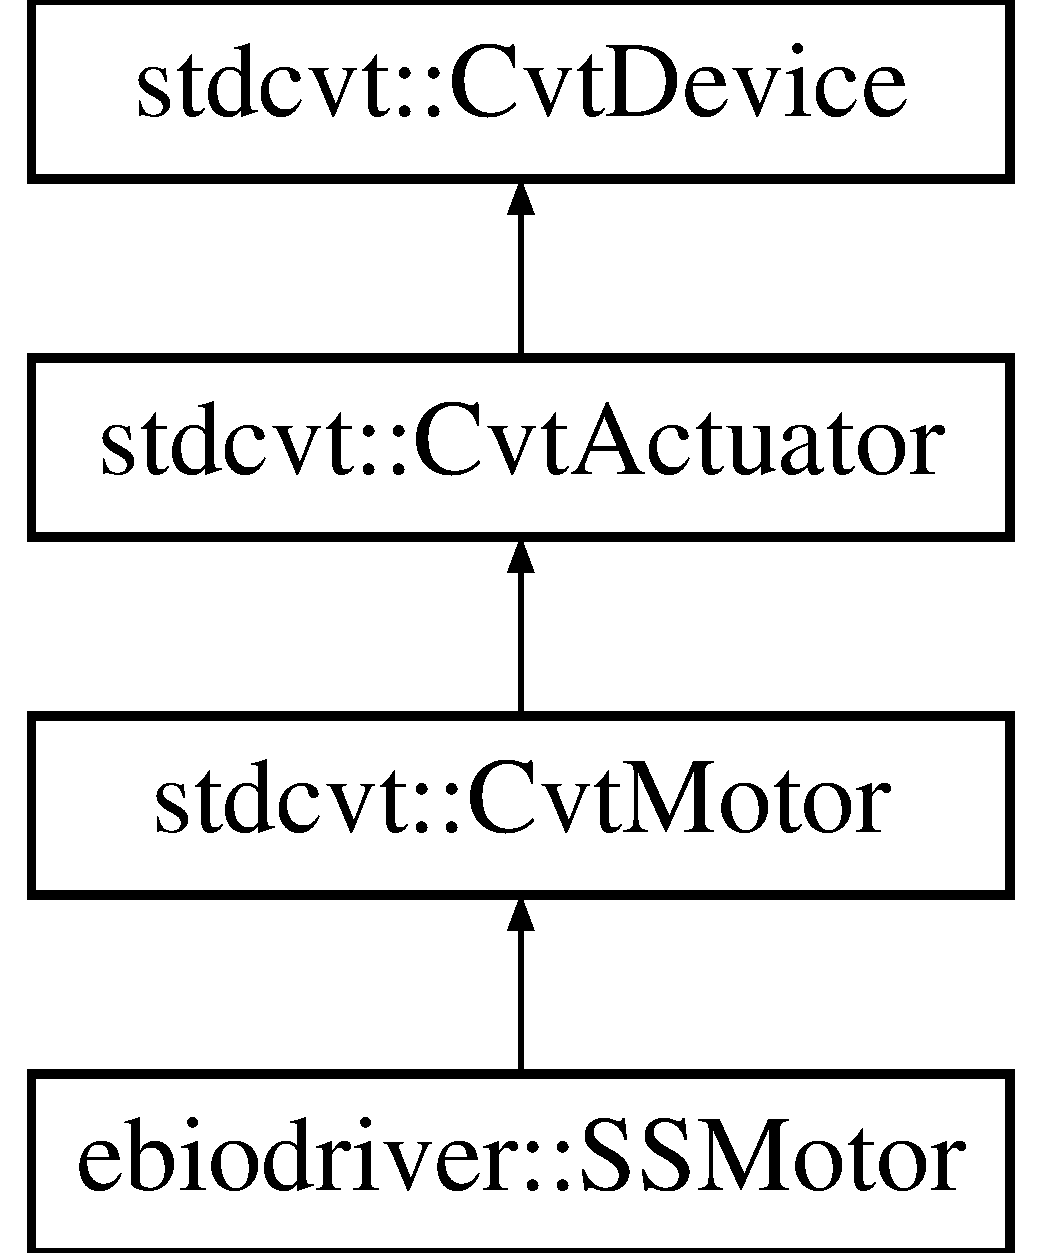
\includegraphics[height=3.000000cm]{classstdcvt_1_1CvtMotor}
\end{center}
\end{figure}
\subsection*{Public 멤버 함수}
\begin{DoxyCompactItemize}
\item 
\hyperlink{classstdcvt_1_1CvtMotor_a5cb552a64668bfbb21d4cd89dd304b6d}{Cvt\+Motor} (int devid, \hyperlink{cvtcode_8h_ae8e34073e35cef0bb47c7fa535fc638b}{devtype\+\_\+t} devtype, \hyperlink{cvtcode_8h_a268eebb73363e24b9e65fd51973bd9c0}{devsec\+\_\+t} section, \hyperlink{cvtcode_8h_a2b37fd5cc4d40c0b8c4b987c271e5ceb}{devtarget\+\_\+t} target, \hyperlink{cvtcode_8h_ad21cd565f839adc5b19a0993e7da7278}{devstat\+\_\+t} devstatus)
\item 
double \hyperlink{classstdcvt_1_1CvtMotor_a5b6c4495daf5aa13b580d9a574c7e866}{setratio} (double ratio)
\item 
double \hyperlink{classstdcvt_1_1CvtMotor_aa6155ea9cba5a0797ce9baa08139c553}{getratio} ()
\item 
string \hyperlink{classstdcvt_1_1CvtMotor_a93295bdf3c61854878f663fad712adaa}{tostring} ()
\end{DoxyCompactItemize}


\subsection{생성자 \& 소멸자 문서화}
\index{stdcvt\+::\+Cvt\+Motor@{stdcvt\+::\+Cvt\+Motor}!Cvt\+Motor@{Cvt\+Motor}}
\index{Cvt\+Motor@{Cvt\+Motor}!stdcvt\+::\+Cvt\+Motor@{stdcvt\+::\+Cvt\+Motor}}
\subsubsection[{\texorpdfstring{Cvt\+Motor(int devid, devtype\+\_\+t devtype, devsec\+\_\+t section, devtarget\+\_\+t target, devstat\+\_\+t devstatus)}{CvtMotor(int devid, devtype_t devtype, devsec_t section, devtarget_t target, devstat_t devstatus)}}]{\setlength{\rightskip}{0pt plus 5cm}stdcvt\+::\+Cvt\+Motor\+::\+Cvt\+Motor (
\begin{DoxyParamCaption}
\item[{int}]{devid, }
\item[{{\bf devtype\+\_\+t}}]{devtype, }
\item[{{\bf devsec\+\_\+t}}]{section, }
\item[{{\bf devtarget\+\_\+t}}]{target, }
\item[{{\bf devstat\+\_\+t}}]{devstatus}
\end{DoxyParamCaption}
)\hspace{0.3cm}{\ttfamily [inline]}}\hypertarget{classstdcvt_1_1CvtMotor_a5cb552a64668bfbb21d4cd89dd304b6d}{}\label{classstdcvt_1_1CvtMotor_a5cb552a64668bfbb21d4cd89dd304b6d}
새로운 모터형 구동기를 생성한다. 
\begin{DoxyParams}{매개변수}
{\em devid} & 장비의 아이디 \\
\hline
{\em devtype} & 장비의 종류 \\
\hline
{\em section} & 장비 설치 구역 \\
\hline
{\em target} & 장비의 대상 \\
\hline
{\em devstatus} & 장비의 상태 \\
\hline
\end{DoxyParams}


\subsection{멤버 함수 문서화}
\index{stdcvt\+::\+Cvt\+Motor@{stdcvt\+::\+Cvt\+Motor}!getratio@{getratio}}
\index{getratio@{getratio}!stdcvt\+::\+Cvt\+Motor@{stdcvt\+::\+Cvt\+Motor}}
\subsubsection[{\texorpdfstring{getratio()}{getratio()}}]{\setlength{\rightskip}{0pt plus 5cm}double stdcvt\+::\+Cvt\+Motor\+::getratio (
\begin{DoxyParamCaption}
{}
\end{DoxyParamCaption}
)\hspace{0.3cm}{\ttfamily [inline]}}\hypertarget{classstdcvt_1_1CvtMotor_aa6155ea9cba5a0797ce9baa08139c553}{}\label{classstdcvt_1_1CvtMotor_aa6155ea9cba5a0797ce9baa08139c553}
모터형 구동기의 위치를 확인한다. \begin{DoxyReturn}{반환값}
구동기의 위치 
\end{DoxyReturn}
\index{stdcvt\+::\+Cvt\+Motor@{stdcvt\+::\+Cvt\+Motor}!setratio@{setratio}}
\index{setratio@{setratio}!stdcvt\+::\+Cvt\+Motor@{stdcvt\+::\+Cvt\+Motor}}
\subsubsection[{\texorpdfstring{setratio(double ratio)}{setratio(double ratio)}}]{\setlength{\rightskip}{0pt plus 5cm}double stdcvt\+::\+Cvt\+Motor\+::setratio (
\begin{DoxyParamCaption}
\item[{double}]{ratio}
\end{DoxyParamCaption}
)\hspace{0.3cm}{\ttfamily [inline]}}\hypertarget{classstdcvt_1_1CvtMotor_a5b6c4495daf5aa13b580d9a574c7e866}{}\label{classstdcvt_1_1CvtMotor_a5b6c4495daf5aa13b580d9a574c7e866}
모터형 구동기의 위치를 세팅한다. 
\begin{DoxyParams}{매개변수}
{\em ratio} & 세팅할 위치 \\
\hline
\end{DoxyParams}
\begin{DoxyReturn}{반환값}
세팅된 위치 
\end{DoxyReturn}
\index{stdcvt\+::\+Cvt\+Motor@{stdcvt\+::\+Cvt\+Motor}!tostring@{tostring}}
\index{tostring@{tostring}!stdcvt\+::\+Cvt\+Motor@{stdcvt\+::\+Cvt\+Motor}}
\subsubsection[{\texorpdfstring{tostring()}{tostring()}}]{\setlength{\rightskip}{0pt plus 5cm}string stdcvt\+::\+Cvt\+Motor\+::tostring (
\begin{DoxyParamCaption}
{}
\end{DoxyParamCaption}
)\hspace{0.3cm}{\ttfamily [inline]}}\hypertarget{classstdcvt_1_1CvtMotor_a93295bdf3c61854878f663fad712adaa}{}\label{classstdcvt_1_1CvtMotor_a93295bdf3c61854878f663fad712adaa}
모터형 구동기의 상태를 문자열로 내보낸다. 

이 클래스에 대한 문서화 페이지는 다음의 파일로부터 생성되었습니다.\+:\begin{DoxyCompactItemize}
\item 
spec/\hyperlink{cvtdevice_8h}{cvtdevice.\+h}\end{DoxyCompactItemize}

\hypertarget{classstdcvt_1_1CvtOption}{}\section{stdcvt\+:\+:Cvt\+Option 클래스 참조}
\label{classstdcvt_1_1CvtOption}\index{stdcvt\+::\+Cvt\+Option@{stdcvt\+::\+Cvt\+Option}}
\subsection*{Public 멤버 함수}
\begin{DoxyCompactItemize}
\item 
\hyperlink{classstdcvt_1_1CvtOption_ad649195a46bae2714aafe069084bea7a}{Cvt\+Option} (json $\ast$poption)
\item 
json \hyperlink{classstdcvt_1_1CvtOption_a912926db2ba4ae39269cdbdfcd0a82b4}{getjson} (string path)
\item 
string \hyperlink{classstdcvt_1_1CvtOption_add9602ed4e44ebb336dcb177b19210d2}{get} (string key)
\item 
double \hyperlink{classstdcvt_1_1CvtOption_a04d78e7d48c97fd268638cb16ec72e7b}{getdouble} (string key)
\item 
int \hyperlink{classstdcvt_1_1CvtOption_a769258713a6968362866a3a8b7753acd}{getint} (string key)
\item 
void $\ast$ \hyperlink{classstdcvt_1_1CvtOption_add9d9f444a0cc5fcbf476cc87abd4de4}{getobject} (string key)
\item 
void $\ast$ \hyperlink{classstdcvt_1_1CvtOption_a552fcb035d6288e44cd3f5da11be28aa}{setobject} (string key, void $\ast$object)
\end{DoxyCompactItemize}


\subsection{생성자 \& 소멸자 문서화}
\index{stdcvt\+::\+Cvt\+Option@{stdcvt\+::\+Cvt\+Option}!Cvt\+Option@{Cvt\+Option}}
\index{Cvt\+Option@{Cvt\+Option}!stdcvt\+::\+Cvt\+Option@{stdcvt\+::\+Cvt\+Option}}
\subsubsection[{\texorpdfstring{Cvt\+Option(json $\ast$poption)}{CvtOption(json *poption)}}]{\setlength{\rightskip}{0pt plus 5cm}stdcvt\+::\+Cvt\+Option\+::\+Cvt\+Option (
\begin{DoxyParamCaption}
\item[{json $\ast$}]{poption}
\end{DoxyParamCaption}
)\hspace{0.3cm}{\ttfamily [inline]}}\hypertarget{classstdcvt_1_1CvtOption_ad649195a46bae2714aafe069084bea7a}{}\label{classstdcvt_1_1CvtOption_ad649195a46bae2714aafe069084bea7a}
새로운 옵션를 생성한다. 
\begin{DoxyParams}{매개변수}
{\em poption} & 특정 드라이버를 위한 옵션. json 타입의 포인터. \\
\hline
\end{DoxyParams}


\subsection{멤버 함수 문서화}
\index{stdcvt\+::\+Cvt\+Option@{stdcvt\+::\+Cvt\+Option}!get@{get}}
\index{get@{get}!stdcvt\+::\+Cvt\+Option@{stdcvt\+::\+Cvt\+Option}}
\subsubsection[{\texorpdfstring{get(string key)}{get(string key)}}]{\setlength{\rightskip}{0pt plus 5cm}string stdcvt\+::\+Cvt\+Option\+::get (
\begin{DoxyParamCaption}
\item[{string}]{key}
\end{DoxyParamCaption}
)\hspace{0.3cm}{\ttfamily [inline]}}\hypertarget{classstdcvt_1_1CvtOption_add9602ed4e44ebb336dcb177b19210d2}{}\label{classstdcvt_1_1CvtOption_add9602ed4e44ebb336dcb177b19210d2}
옵션의 값을 문자열로 리턴한다. 
\begin{DoxyParams}{매개변수}
{\em key} & 옵션을 선택하기 위한 키 \\
\hline
\end{DoxyParams}
\begin{DoxyReturn}{반환값}
옵션의 문자열 값 
\end{DoxyReturn}
\index{stdcvt\+::\+Cvt\+Option@{stdcvt\+::\+Cvt\+Option}!getdouble@{getdouble}}
\index{getdouble@{getdouble}!stdcvt\+::\+Cvt\+Option@{stdcvt\+::\+Cvt\+Option}}
\subsubsection[{\texorpdfstring{getdouble(string key)}{getdouble(string key)}}]{\setlength{\rightskip}{0pt plus 5cm}double stdcvt\+::\+Cvt\+Option\+::getdouble (
\begin{DoxyParamCaption}
\item[{string}]{key}
\end{DoxyParamCaption}
)\hspace{0.3cm}{\ttfamily [inline]}}\hypertarget{classstdcvt_1_1CvtOption_a04d78e7d48c97fd268638cb16ec72e7b}{}\label{classstdcvt_1_1CvtOption_a04d78e7d48c97fd268638cb16ec72e7b}
옵션의 값을 실수형으로 리턴한다. 
\begin{DoxyParams}{매개변수}
{\em key} & 옵션을 선택하기 위한 키 \\
\hline
\end{DoxyParams}
\begin{DoxyReturn}{반환값}
옵션의 실수형값 
\end{DoxyReturn}
\index{stdcvt\+::\+Cvt\+Option@{stdcvt\+::\+Cvt\+Option}!getint@{getint}}
\index{getint@{getint}!stdcvt\+::\+Cvt\+Option@{stdcvt\+::\+Cvt\+Option}}
\subsubsection[{\texorpdfstring{getint(string key)}{getint(string key)}}]{\setlength{\rightskip}{0pt plus 5cm}int stdcvt\+::\+Cvt\+Option\+::getint (
\begin{DoxyParamCaption}
\item[{string}]{key}
\end{DoxyParamCaption}
)\hspace{0.3cm}{\ttfamily [inline]}}\hypertarget{classstdcvt_1_1CvtOption_a769258713a6968362866a3a8b7753acd}{}\label{classstdcvt_1_1CvtOption_a769258713a6968362866a3a8b7753acd}
옵션의 값을 정수형으로 리턴한다. 
\begin{DoxyParams}{매개변수}
{\em key} & 옵션을 선택하기 위한 키 \\
\hline
\end{DoxyParams}
\begin{DoxyReturn}{반환값}
옵션의 값 
\end{DoxyReturn}
\index{stdcvt\+::\+Cvt\+Option@{stdcvt\+::\+Cvt\+Option}!getjson@{getjson}}
\index{getjson@{getjson}!stdcvt\+::\+Cvt\+Option@{stdcvt\+::\+Cvt\+Option}}
\subsubsection[{\texorpdfstring{getjson(string path)}{getjson(string path)}}]{\setlength{\rightskip}{0pt plus 5cm}json stdcvt\+::\+Cvt\+Option\+::getjson (
\begin{DoxyParamCaption}
\item[{string}]{path}
\end{DoxyParamCaption}
)\hspace{0.3cm}{\ttfamily [inline]}}\hypertarget{classstdcvt_1_1CvtOption_a912926db2ba4ae39269cdbdfcd0a82b4}{}\label{classstdcvt_1_1CvtOption_a912926db2ba4ae39269cdbdfcd0a82b4}
복잡한 옵션을 사용하고자 할때에는 옵션의 값을 리턴한다. 
\begin{DoxyParams}{매개변수}
{\em } & \\
\hline
\end{DoxyParams}
\index{stdcvt\+::\+Cvt\+Option@{stdcvt\+::\+Cvt\+Option}!getobject@{getobject}}
\index{getobject@{getobject}!stdcvt\+::\+Cvt\+Option@{stdcvt\+::\+Cvt\+Option}}
\subsubsection[{\texorpdfstring{getobject(string key)}{getobject(string key)}}]{\setlength{\rightskip}{0pt plus 5cm}void$\ast$ stdcvt\+::\+Cvt\+Option\+::getobject (
\begin{DoxyParamCaption}
\item[{string}]{key}
\end{DoxyParamCaption}
)\hspace{0.3cm}{\ttfamily [inline]}}\hypertarget{classstdcvt_1_1CvtOption_add9d9f444a0cc5fcbf476cc87abd4de4}{}\label{classstdcvt_1_1CvtOption_add9d9f444a0cc5fcbf476cc87abd4de4}
옵션의 값을 void $\ast$로 리턴한다. 
\begin{DoxyParams}{매개변수}
{\em key} & 옵션을 선택하기 위한 키 \\
\hline
\end{DoxyParams}
\begin{DoxyReturn}{반환값}
옵션의 값 
\end{DoxyReturn}
\index{stdcvt\+::\+Cvt\+Option@{stdcvt\+::\+Cvt\+Option}!setobject@{setobject}}
\index{setobject@{setobject}!stdcvt\+::\+Cvt\+Option@{stdcvt\+::\+Cvt\+Option}}
\subsubsection[{\texorpdfstring{setobject(string key, void $\ast$object)}{setobject(string key, void *object)}}]{\setlength{\rightskip}{0pt plus 5cm}void$\ast$ stdcvt\+::\+Cvt\+Option\+::setobject (
\begin{DoxyParamCaption}
\item[{string}]{key, }
\item[{void $\ast$}]{object}
\end{DoxyParamCaption}
)\hspace{0.3cm}{\ttfamily [inline]}}\hypertarget{classstdcvt_1_1CvtOption_a552fcb035d6288e44cd3f5da11be28aa}{}\label{classstdcvt_1_1CvtOption_a552fcb035d6288e44cd3f5da11be28aa}
옵션의 값을 세팅한다. 
\begin{DoxyParams}{매개변수}
{\em key} & 옵션을 선택하기 위한 키 \\
\hline
{\em object} & 옵션값 \\
\hline
\end{DoxyParams}
\begin{DoxyReturn}{반환값}
옵션의 값 
\end{DoxyReturn}


이 클래스에 대한 문서화 페이지는 다음의 파일로부터 생성되었습니다.\+:\begin{DoxyCompactItemize}
\item 
spec/\hyperlink{cvtoption_8h}{cvtoption.\+h}\end{DoxyCompactItemize}

\hypertarget{classstdcvt_1_1CvtRatioCommand}{}\section{stdcvt\+:\+:Cvt\+Ratio\+Command 클래스 참조}
\label{classstdcvt_1_1CvtRatioCommand}\index{stdcvt\+::\+Cvt\+Ratio\+Command@{stdcvt\+::\+Cvt\+Ratio\+Command}}
stdcvt\+:\+:Cvt\+Ratio\+Command에 대한 상속 다이어그램 \+: \begin{figure}[H]
\begin{center}
\leavevmode
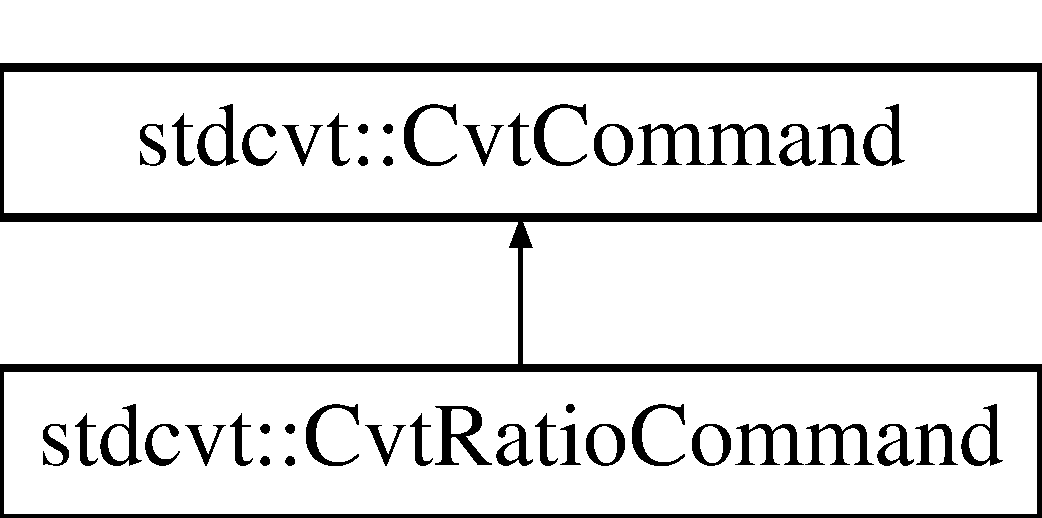
\includegraphics[height=2.000000cm]{classstdcvt_1_1CvtRatioCommand}
\end{center}
\end{figure}
\subsection*{Public 멤버 함수}
\begin{DoxyCompactItemize}
\item 
\hyperlink{classstdcvt_1_1CvtRatioCommand_a5bb6b4eb195f659cab02a613f206b075}{Cvt\+Ratio\+Command} (int cmdid, \hyperlink{classstdcvt_1_1CvtDeviceSpec}{Cvt\+Device\+Spec} $\ast$pdevspec, bool onoff, double ratio)
\item 
double \hyperlink{classstdcvt_1_1CvtRatioCommand_a4c16b3d69d2c85ee1efe889092c351b4}{getratio} ()
\end{DoxyCompactItemize}


\subsection{생성자 \& 소멸자 문서화}
\index{stdcvt\+::\+Cvt\+Ratio\+Command@{stdcvt\+::\+Cvt\+Ratio\+Command}!Cvt\+Ratio\+Command@{Cvt\+Ratio\+Command}}
\index{Cvt\+Ratio\+Command@{Cvt\+Ratio\+Command}!stdcvt\+::\+Cvt\+Ratio\+Command@{stdcvt\+::\+Cvt\+Ratio\+Command}}
\subsubsection[{\texorpdfstring{Cvt\+Ratio\+Command(int cmdid, Cvt\+Device\+Spec $\ast$pdevspec, bool onoff, double ratio)}{CvtRatioCommand(int cmdid, CvtDeviceSpec *pdevspec, bool onoff, double ratio)}}]{\setlength{\rightskip}{0pt plus 5cm}stdcvt\+::\+Cvt\+Ratio\+Command\+::\+Cvt\+Ratio\+Command (
\begin{DoxyParamCaption}
\item[{int}]{cmdid, }
\item[{{\bf Cvt\+Device\+Spec} $\ast$}]{pdevspec, }
\item[{bool}]{onoff, }
\item[{double}]{ratio}
\end{DoxyParamCaption}
)\hspace{0.3cm}{\ttfamily [inline]}}\hypertarget{classstdcvt_1_1CvtRatioCommand_a5bb6b4eb195f659cab02a613f206b075}{}\label{classstdcvt_1_1CvtRatioCommand_a5bb6b4eb195f659cab02a613f206b075}
새로운 명령를 생성한다. 
\begin{DoxyParams}{매개변수}
{\em cmdid} & 명령의 아이디 \\
\hline
{\em pdevspec} & 명령을 수행할 장비스펙의 포인터 \\
\hline
{\em onoff} & 작동상태 \\
\hline
{\em ratio} & 지정된 비율 \\
\hline
\end{DoxyParams}


\subsection{멤버 함수 문서화}
\index{stdcvt\+::\+Cvt\+Ratio\+Command@{stdcvt\+::\+Cvt\+Ratio\+Command}!getratio@{getratio}}
\index{getratio@{getratio}!stdcvt\+::\+Cvt\+Ratio\+Command@{stdcvt\+::\+Cvt\+Ratio\+Command}}
\subsubsection[{\texorpdfstring{getratio()}{getratio()}}]{\setlength{\rightskip}{0pt plus 5cm}double stdcvt\+::\+Cvt\+Ratio\+Command\+::getratio (
\begin{DoxyParamCaption}
{}
\end{DoxyParamCaption}
)\hspace{0.3cm}{\ttfamily [inline]}}\hypertarget{classstdcvt_1_1CvtRatioCommand_a4c16b3d69d2c85ee1efe889092c351b4}{}\label{classstdcvt_1_1CvtRatioCommand_a4c16b3d69d2c85ee1efe889092c351b4}
지정된 비율값을 확인한다. \begin{DoxyReturn}{반환값}
ratio 값 
\end{DoxyReturn}


이 클래스에 대한 문서화 페이지는 다음의 파일로부터 생성되었습니다.\+:\begin{DoxyCompactItemize}
\item 
spec/\hyperlink{cvtcommand_8h}{cvtcommand.\+h}\end{DoxyCompactItemize}

\hypertarget{classstdcvt_1_1CvtRawCommand}{}\section{stdcvt\+:\+:Cvt\+Raw\+Command 클래스 참조}
\label{classstdcvt_1_1CvtRawCommand}\index{stdcvt\+::\+Cvt\+Raw\+Command@{stdcvt\+::\+Cvt\+Raw\+Command}}
stdcvt\+:\+:Cvt\+Raw\+Command에 대한 상속 다이어그램 \+: \begin{figure}[H]
\begin{center}
\leavevmode
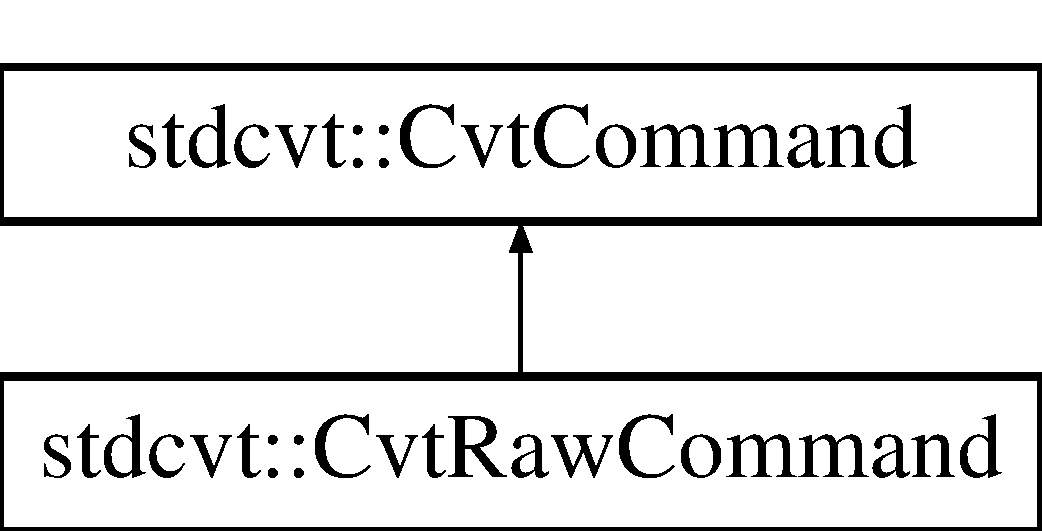
\includegraphics[height=2.000000cm]{classstdcvt_1_1CvtRawCommand}
\end{center}
\end{figure}
\subsection*{Public 멤버 함수}
\begin{DoxyCompactItemize}
\item 
\hyperlink{classstdcvt_1_1CvtRawCommand_ae42522abd4b67a651ecdc04b9ca53862}{Cvt\+Raw\+Command} (int cmdid, \hyperlink{classstdcvt_1_1CvtDeviceSpec}{Cvt\+Device\+Spec} $\ast$pdevspec, bool onoff, int modelcode, string devid, string arg)
\item 
int \hyperlink{classstdcvt_1_1CvtRawCommand_ad7377cc0531f970032368e5518211e8c}{getmodelcode} ()
\item 
string \hyperlink{classstdcvt_1_1CvtRawCommand_a1ea00736911fff856e7d01b9fbd6d49d}{getdevid} ()
\item 
string \hyperlink{classstdcvt_1_1CvtRawCommand_a2429ee7b28de85a56203666d6aeda6de}{getarg} ()
\end{DoxyCompactItemize}


\subsection{생성자 \& 소멸자 문서화}
\index{stdcvt\+::\+Cvt\+Raw\+Command@{stdcvt\+::\+Cvt\+Raw\+Command}!Cvt\+Raw\+Command@{Cvt\+Raw\+Command}}
\index{Cvt\+Raw\+Command@{Cvt\+Raw\+Command}!stdcvt\+::\+Cvt\+Raw\+Command@{stdcvt\+::\+Cvt\+Raw\+Command}}
\subsubsection[{\texorpdfstring{Cvt\+Raw\+Command(int cmdid, Cvt\+Device\+Spec $\ast$pdevspec, bool onoff, int modelcode, string devid, string arg)}{CvtRawCommand(int cmdid, CvtDeviceSpec *pdevspec, bool onoff, int modelcode, string devid, string arg)}}]{\setlength{\rightskip}{0pt plus 5cm}stdcvt\+::\+Cvt\+Raw\+Command\+::\+Cvt\+Raw\+Command (
\begin{DoxyParamCaption}
\item[{int}]{cmdid, }
\item[{{\bf Cvt\+Device\+Spec} $\ast$}]{pdevspec, }
\item[{bool}]{onoff, }
\item[{int}]{modelcode, }
\item[{string}]{devid, }
\item[{string}]{arg}
\end{DoxyParamCaption}
)\hspace{0.3cm}{\ttfamily [inline]}}\hypertarget{classstdcvt_1_1CvtRawCommand_ae42522abd4b67a651ecdc04b9ca53862}{}\label{classstdcvt_1_1CvtRawCommand_ae42522abd4b67a651ecdc04b9ca53862}
새로운 명령를 생성한다. 
\begin{DoxyParams}{매개변수}
{\em cmdid} & 명령의 아이디 \\
\hline
{\em pdevspec} & 명령을 수행할 장비스펙의 포인터 \\
\hline
{\em onoff} & 작동상태 \\
\hline
{\em modelcode} & 명령의 인자를 해석할 수 있는 드라이버의 모델코드 \\
\hline
{\em devid} & 명령을 수행할 장비의 아이디 \\
\hline
{\em arg} & 명령의 인자. 문자열 형으로 꼭 base64 인코딩 되어 있어야 함. \\
\hline
\end{DoxyParams}


\subsection{멤버 함수 문서화}
\index{stdcvt\+::\+Cvt\+Raw\+Command@{stdcvt\+::\+Cvt\+Raw\+Command}!getarg@{getarg}}
\index{getarg@{getarg}!stdcvt\+::\+Cvt\+Raw\+Command@{stdcvt\+::\+Cvt\+Raw\+Command}}
\subsubsection[{\texorpdfstring{getarg()}{getarg()}}]{\setlength{\rightskip}{0pt plus 5cm}string stdcvt\+::\+Cvt\+Raw\+Command\+::getarg (
\begin{DoxyParamCaption}
{}
\end{DoxyParamCaption}
)\hspace{0.3cm}{\ttfamily [inline]}}\hypertarget{classstdcvt_1_1CvtRawCommand_a2429ee7b28de85a56203666d6aeda6de}{}\label{classstdcvt_1_1CvtRawCommand_a2429ee7b28de85a56203666d6aeda6de}
명령 수행을 위한 인자를 확인한다. \begin{DoxyReturn}{반환값}
명령 인자값 
\end{DoxyReturn}
\index{stdcvt\+::\+Cvt\+Raw\+Command@{stdcvt\+::\+Cvt\+Raw\+Command}!getdevid@{getdevid}}
\index{getdevid@{getdevid}!stdcvt\+::\+Cvt\+Raw\+Command@{stdcvt\+::\+Cvt\+Raw\+Command}}
\subsubsection[{\texorpdfstring{getdevid()}{getdevid()}}]{\setlength{\rightskip}{0pt plus 5cm}string stdcvt\+::\+Cvt\+Raw\+Command\+::getdevid (
\begin{DoxyParamCaption}
{}
\end{DoxyParamCaption}
)\hspace{0.3cm}{\ttfamily [inline]}}\hypertarget{classstdcvt_1_1CvtRawCommand_a1ea00736911fff856e7d01b9fbd6d49d}{}\label{classstdcvt_1_1CvtRawCommand_a1ea00736911fff856e7d01b9fbd6d49d}
명령을 수행할 장비의 아이디를 확인한다. \begin{DoxyReturn}{반환값}
장비아이디값 
\end{DoxyReturn}
\index{stdcvt\+::\+Cvt\+Raw\+Command@{stdcvt\+::\+Cvt\+Raw\+Command}!getmodelcode@{getmodelcode}}
\index{getmodelcode@{getmodelcode}!stdcvt\+::\+Cvt\+Raw\+Command@{stdcvt\+::\+Cvt\+Raw\+Command}}
\subsubsection[{\texorpdfstring{getmodelcode()}{getmodelcode()}}]{\setlength{\rightskip}{0pt plus 5cm}int stdcvt\+::\+Cvt\+Raw\+Command\+::getmodelcode (
\begin{DoxyParamCaption}
{}
\end{DoxyParamCaption}
)\hspace{0.3cm}{\ttfamily [inline]}}\hypertarget{classstdcvt_1_1CvtRawCommand_ad7377cc0531f970032368e5518211e8c}{}\label{classstdcvt_1_1CvtRawCommand_ad7377cc0531f970032368e5518211e8c}
명령에 할당된 모델코드를 확인한다. \begin{DoxyReturn}{반환값}
모델코드값 
\end{DoxyReturn}


이 클래스에 대한 문서화 페이지는 다음의 파일로부터 생성되었습니다.\+:\begin{DoxyCompactItemize}
\item 
spec/\hyperlink{cvtcommand_8h}{cvtcommand.\+h}\end{DoxyCompactItemize}

\hypertarget{classstdcvt_1_1CvtSensor}{}\section{stdcvt\+:\+:Cvt\+Sensor 클래스 참조}
\label{classstdcvt_1_1CvtSensor}\index{stdcvt\+::\+Cvt\+Sensor@{stdcvt\+::\+Cvt\+Sensor}}
stdcvt\+:\+:Cvt\+Sensor에 대한 상속 다이어그램 \+: \begin{figure}[H]
\begin{center}
\leavevmode
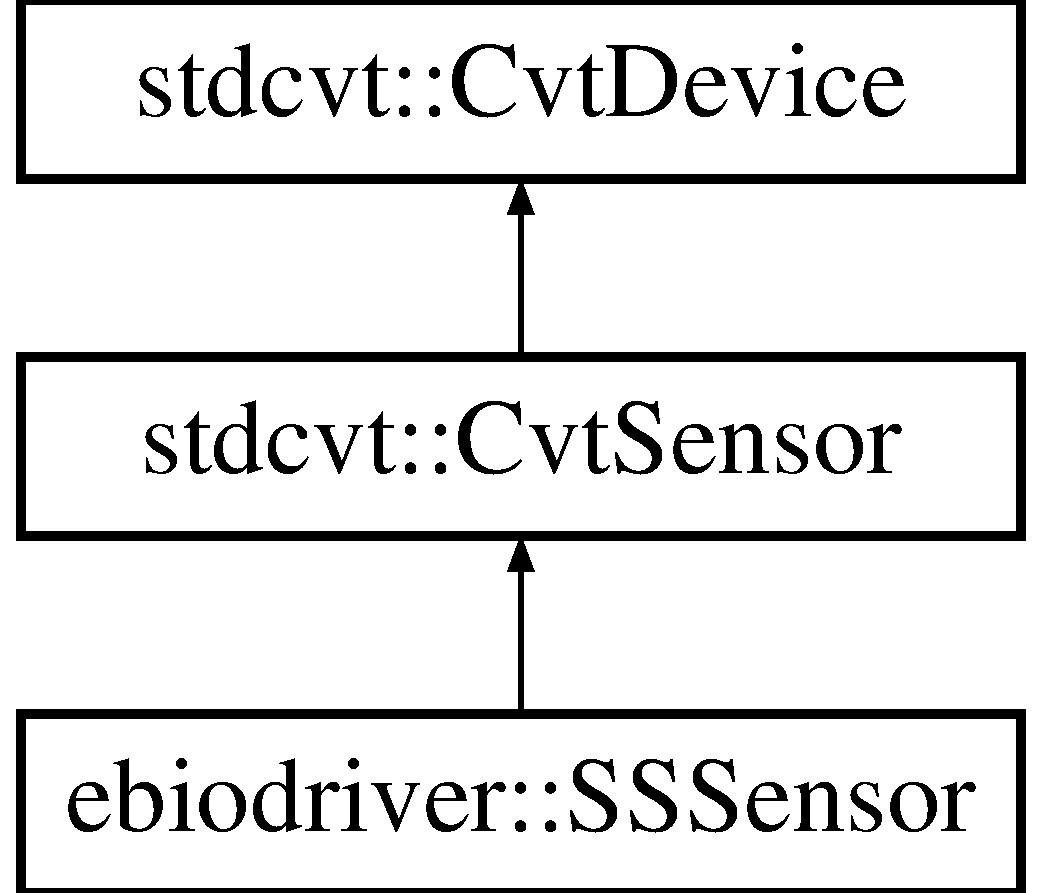
\includegraphics[height=3.000000cm]{classstdcvt_1_1CvtSensor}
\end{center}
\end{figure}
\subsection*{Public 멤버 함수}
\begin{DoxyCompactItemize}
\item 
\hyperlink{classstdcvt_1_1CvtSensor_a55d2db9b5706a0b94cb92be54328cd1f}{Cvt\+Sensor} (int devid, \hyperlink{cvtcode_8h_ae8e34073e35cef0bb47c7fa535fc638b}{devtype\+\_\+t} devtype, \hyperlink{cvtcode_8h_a268eebb73363e24b9e65fd51973bd9c0}{devsec\+\_\+t} section, \hyperlink{cvtcode_8h_a2b37fd5cc4d40c0b8c4b987c271e5ceb}{devtarget\+\_\+t} target, \hyperlink{cvtcode_8h_ad21cd565f839adc5b19a0993e7da7278}{devstat\+\_\+t} devstatus, \hyperlink{cvtcode_8h_a6d4ed81d95144c5eedcd08eda1e800a4}{obsunit\+\_\+t} unit)
\item 
\hyperlink{cvtcode_8h_a6d4ed81d95144c5eedcd08eda1e800a4}{obsunit\+\_\+t} \hyperlink{classstdcvt_1_1CvtSensor_ac4342e95b9977063bb4e37ce1418759c}{getunit} ()
\item 
\hyperlink{cvtcode_8h_a6d4ed81d95144c5eedcd08eda1e800a4}{obsunit\+\_\+t} \hyperlink{classstdcvt_1_1CvtSensor_a0e13dd86635e5077dbadc6c0fe396b5e}{setunit} (\hyperlink{cvtcode_8h_a6d4ed81d95144c5eedcd08eda1e800a4}{obsunit\+\_\+t} unit)
\item 
double \hyperlink{classstdcvt_1_1CvtSensor_aba7a61d2f5fac1c100a17a8831727b29}{writeobservation} (double value)
\item 
double \hyperlink{classstdcvt_1_1CvtSensor_a2d3b6d09f67166af035189b59590cf82}{readobservation} ()
\item 
string \hyperlink{classstdcvt_1_1CvtSensor_aa9f10c534408e35f1d761941a8320e50}{tostring} ()
\end{DoxyCompactItemize}


\subsection{생성자 \& 소멸자 문서화}
\index{stdcvt\+::\+Cvt\+Sensor@{stdcvt\+::\+Cvt\+Sensor}!Cvt\+Sensor@{Cvt\+Sensor}}
\index{Cvt\+Sensor@{Cvt\+Sensor}!stdcvt\+::\+Cvt\+Sensor@{stdcvt\+::\+Cvt\+Sensor}}
\subsubsection[{\texorpdfstring{Cvt\+Sensor(int devid, devtype\+\_\+t devtype, devsec\+\_\+t section, devtarget\+\_\+t target, devstat\+\_\+t devstatus, obsunit\+\_\+t unit)}{CvtSensor(int devid, devtype_t devtype, devsec_t section, devtarget_t target, devstat_t devstatus, obsunit_t unit)}}]{\setlength{\rightskip}{0pt plus 5cm}stdcvt\+::\+Cvt\+Sensor\+::\+Cvt\+Sensor (
\begin{DoxyParamCaption}
\item[{int}]{devid, }
\item[{{\bf devtype\+\_\+t}}]{devtype, }
\item[{{\bf devsec\+\_\+t}}]{section, }
\item[{{\bf devtarget\+\_\+t}}]{target, }
\item[{{\bf devstat\+\_\+t}}]{devstatus, }
\item[{{\bf obsunit\+\_\+t}}]{unit}
\end{DoxyParamCaption}
)\hspace{0.3cm}{\ttfamily [inline]}}\hypertarget{classstdcvt_1_1CvtSensor_a55d2db9b5706a0b94cb92be54328cd1f}{}\label{classstdcvt_1_1CvtSensor_a55d2db9b5706a0b94cb92be54328cd1f}
새로운 센서를 생성한다. 
\begin{DoxyParams}{매개변수}
{\em devid} & 센서의 아이디 \\
\hline
{\em devtype} & 장비의 종류 \\
\hline
{\em section} & 장비 설치 구역 \\
\hline
{\em target} & 장비의 대상 \\
\hline
{\em devstatus} & 센서의 상태 \\
\hline
{\em unit} & 관측치의 단위 \\
\hline
\end{DoxyParams}


\subsection{멤버 함수 문서화}
\index{stdcvt\+::\+Cvt\+Sensor@{stdcvt\+::\+Cvt\+Sensor}!getunit@{getunit}}
\index{getunit@{getunit}!stdcvt\+::\+Cvt\+Sensor@{stdcvt\+::\+Cvt\+Sensor}}
\subsubsection[{\texorpdfstring{getunit()}{getunit()}}]{\setlength{\rightskip}{0pt plus 5cm}{\bf obsunit\+\_\+t} stdcvt\+::\+Cvt\+Sensor\+::getunit (
\begin{DoxyParamCaption}
{}
\end{DoxyParamCaption}
)\hspace{0.3cm}{\ttfamily [inline]}}\hypertarget{classstdcvt_1_1CvtSensor_ac4342e95b9977063bb4e37ce1418759c}{}\label{classstdcvt_1_1CvtSensor_ac4342e95b9977063bb4e37ce1418759c}
관측치 단위를 읽는다. \begin{DoxyReturn}{반환값}
관측치 단위 
\end{DoxyReturn}
\index{stdcvt\+::\+Cvt\+Sensor@{stdcvt\+::\+Cvt\+Sensor}!readobservation@{readobservation}}
\index{readobservation@{readobservation}!stdcvt\+::\+Cvt\+Sensor@{stdcvt\+::\+Cvt\+Sensor}}
\subsubsection[{\texorpdfstring{readobservation()}{readobservation()}}]{\setlength{\rightskip}{0pt plus 5cm}double stdcvt\+::\+Cvt\+Sensor\+::readobservation (
\begin{DoxyParamCaption}
{}
\end{DoxyParamCaption}
)\hspace{0.3cm}{\ttfamily [inline]}}\hypertarget{classstdcvt_1_1CvtSensor_a2d3b6d09f67166af035189b59590cf82}{}\label{classstdcvt_1_1CvtSensor_a2d3b6d09f67166af035189b59590cf82}
관측치를 읽는다. \begin{DoxyReturn}{반환값}
관측치값 
\end{DoxyReturn}
\index{stdcvt\+::\+Cvt\+Sensor@{stdcvt\+::\+Cvt\+Sensor}!setunit@{setunit}}
\index{setunit@{setunit}!stdcvt\+::\+Cvt\+Sensor@{stdcvt\+::\+Cvt\+Sensor}}
\subsubsection[{\texorpdfstring{setunit(obsunit\+\_\+t unit)}{setunit(obsunit_t unit)}}]{\setlength{\rightskip}{0pt plus 5cm}{\bf obsunit\+\_\+t} stdcvt\+::\+Cvt\+Sensor\+::setunit (
\begin{DoxyParamCaption}
\item[{{\bf obsunit\+\_\+t}}]{unit}
\end{DoxyParamCaption}
)\hspace{0.3cm}{\ttfamily [inline]}}\hypertarget{classstdcvt_1_1CvtSensor_a0e13dd86635e5077dbadc6c0fe396b5e}{}\label{classstdcvt_1_1CvtSensor_a0e13dd86635e5077dbadc6c0fe396b5e}
관측치 단위를 세팅한다. 
\begin{DoxyParams}{매개변수}
{\em unit} & 새로 세팅할 관측치 단위 \\
\hline
\end{DoxyParams}
\begin{DoxyReturn}{반환값}
관측치 단위 
\end{DoxyReturn}
\index{stdcvt\+::\+Cvt\+Sensor@{stdcvt\+::\+Cvt\+Sensor}!tostring@{tostring}}
\index{tostring@{tostring}!stdcvt\+::\+Cvt\+Sensor@{stdcvt\+::\+Cvt\+Sensor}}
\subsubsection[{\texorpdfstring{tostring()}{tostring()}}]{\setlength{\rightskip}{0pt plus 5cm}string stdcvt\+::\+Cvt\+Sensor\+::tostring (
\begin{DoxyParamCaption}
{}
\end{DoxyParamCaption}
)\hspace{0.3cm}{\ttfamily [inline]}}\hypertarget{classstdcvt_1_1CvtSensor_aa9f10c534408e35f1d761941a8320e50}{}\label{classstdcvt_1_1CvtSensor_aa9f10c534408e35f1d761941a8320e50}
센서의 상태를 문자열로 내보낸다. \index{stdcvt\+::\+Cvt\+Sensor@{stdcvt\+::\+Cvt\+Sensor}!writeobservation@{writeobservation}}
\index{writeobservation@{writeobservation}!stdcvt\+::\+Cvt\+Sensor@{stdcvt\+::\+Cvt\+Sensor}}
\subsubsection[{\texorpdfstring{writeobservation(double value)}{writeobservation(double value)}}]{\setlength{\rightskip}{0pt plus 5cm}double stdcvt\+::\+Cvt\+Sensor\+::writeobservation (
\begin{DoxyParamCaption}
\item[{double}]{value}
\end{DoxyParamCaption}
)\hspace{0.3cm}{\ttfamily [inline]}}\hypertarget{classstdcvt_1_1CvtSensor_aba7a61d2f5fac1c100a17a8831727b29}{}\label{classstdcvt_1_1CvtSensor_aba7a61d2f5fac1c100a17a8831727b29}
관측치를 기록한다. 
\begin{DoxyParams}{매개변수}
{\em value} & 관측치 \\
\hline
\end{DoxyParams}
\begin{DoxyReturn}{반환값}
기록한 관측치값 
\end{DoxyReturn}


이 클래스에 대한 문서화 페이지는 다음의 파일로부터 생성되었습니다.\+:\begin{DoxyCompactItemize}
\item 
spec/\hyperlink{cvtdevice_8h}{cvtdevice.\+h}\end{DoxyCompactItemize}

\hypertarget{classstdcvt_1_1CvtSpec}{}\section{stdcvt\+:\+:Cvt\+Spec 클래스 참조}
\label{classstdcvt_1_1CvtSpec}\index{stdcvt\+::\+Cvt\+Spec@{stdcvt\+::\+Cvt\+Spec}}
\subsection*{Public 멤버 함수}
\begin{DoxyCompactItemize}
\item 
\hyperlink{classstdcvt_1_1CvtSpec_a56cea5a84f2cb7cd0089603f3a97d315}{Cvt\+Spec} ()
\end{DoxyCompactItemize}


\subsection{생성자 \& 소멸자 문서화}
\index{stdcvt\+::\+Cvt\+Spec@{stdcvt\+::\+Cvt\+Spec}!Cvt\+Spec@{Cvt\+Spec}}
\index{Cvt\+Spec@{Cvt\+Spec}!stdcvt\+::\+Cvt\+Spec@{stdcvt\+::\+Cvt\+Spec}}
\subsubsection[{\texorpdfstring{Cvt\+Spec()}{CvtSpec()}}]{\setlength{\rightskip}{0pt plus 5cm}stdcvt\+::\+Cvt\+Spec\+::\+Cvt\+Spec (
\begin{DoxyParamCaption}
{}
\end{DoxyParamCaption}
)\hspace{0.3cm}{\ttfamily [inline]}}\hypertarget{classstdcvt_1_1CvtSpec_a56cea5a84f2cb7cd0089603f3a97d315}{}\label{classstdcvt_1_1CvtSpec_a56cea5a84f2cb7cd0089603f3a97d315}
새로운 컨버터스펙을 생성한다. 

이 클래스에 대한 문서화 페이지는 다음의 파일로부터 생성되었습니다.\+:\begin{DoxyCompactItemize}
\item 
spec/\hyperlink{cvtspec_8h}{cvtspec.\+h}\end{DoxyCompactItemize}

\hypertarget{classebiodriver_1_1DSSampleDriver}{}\section{ebiodriver\+:\+:D\+S\+Sample\+Driver 클래스 참조}
\label{classebiodriver_1_1DSSampleDriver}\index{ebiodriver\+::\+D\+S\+Sample\+Driver@{ebiodriver\+::\+D\+S\+Sample\+Driver}}
ebiodriver\+:\+:D\+S\+Sample\+Driver에 대한 상속 다이어그램 \+: \begin{figure}[H]
\begin{center}
\leavevmode
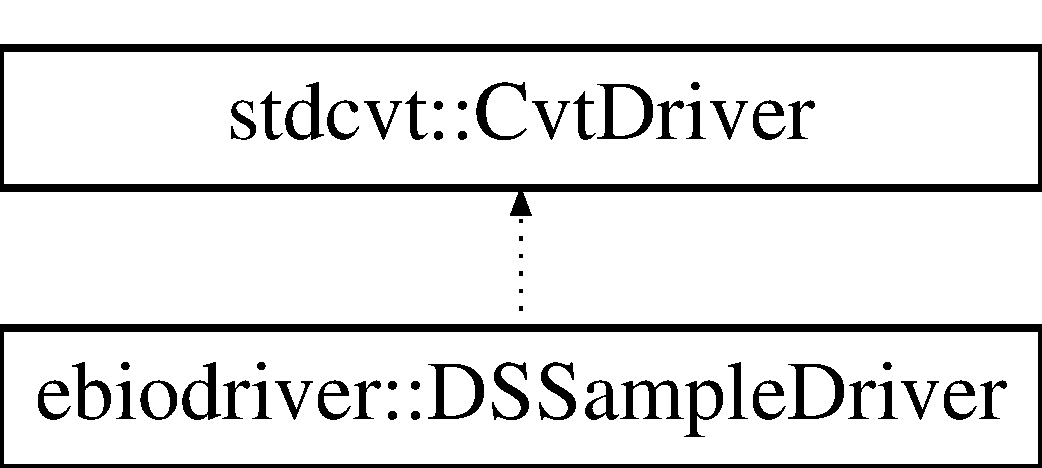
\includegraphics[height=2.000000cm]{classebiodriver_1_1DSSampleDriver}
\end{center}
\end{figure}
\subsection*{Public 멤버 함수}
\begin{DoxyCompactItemize}
\item 
\hyperlink{classebiodriver_1_1DSSampleDriver_ab7b862bbc77a0ebdffde3931e1d889a3}{D\+S\+Sample\+Driver} ()
\item 
string \hyperlink{classebiodriver_1_1DSSampleDriver_ac2173224ee7e59f6386f9dab1a8cb4b6}{getversion} ()
\item 
string \hyperlink{classebiodriver_1_1DSSampleDriver_aa99ba3c94b288a61a07a73393fec0f81}{getmodel} ()
\item 
string \hyperlink{classebiodriver_1_1DSSampleDriver_a6c7281bb4d01245c1b5087a1fbcc2b80}{getcompany} ()
\item 
bool \hyperlink{classebiodriver_1_1DSSampleDriver_aaeb74b5cfe475ecdafe87279574fe6e4}{initialize} (\hyperlink{classstdcvt_1_1CvtOption}{Cvt\+Option} option)
\item 
bool \hyperlink{classebiodriver_1_1DSSampleDriver_a21e12d56a042bc9efee56f9af7e41f7c}{finalize} ()
\item 
bool \hyperlink{classebiodriver_1_1DSSampleDriver_af7463eb1268616f1f2e677d2ad56cf63}{preprocess} ()
\item 
bool \hyperlink{classebiodriver_1_1DSSampleDriver_aa5913df52706dd85fb4d3c0b8e4e5a92}{postprocess} ()
\item 
\hyperlink{classstdcvt_1_1CvtDevice}{Cvt\+Device} $\ast$ \hyperlink{classebiodriver_1_1DSSampleDriver_a3dcd13870509c3139c6c0ad7ba22cbed}{getdevice} (int index)
\item 
bool \hyperlink{classebiodriver_1_1DSSampleDriver_a027286ae7b53a82d8d46731cfabcfea3}{sharedevice} (\hyperlink{classstdcvt_1_1CvtDevice}{Cvt\+Device} $\ast$pdevice)
\item 
\hyperlink{classstdcvt_1_1CvtCommand}{Cvt\+Command} $\ast$ \hyperlink{classebiodriver_1_1DSSampleDriver_acfccb95870864ce6dc5f99ab94c214fa}{getcommand} (int index)
\item 
bool \hyperlink{classebiodriver_1_1DSSampleDriver_a0fe50dbf8dd10f4568f25e83e7e3e873}{control} (\hyperlink{classstdcvt_1_1CvtCommand}{Cvt\+Command} $\ast$pcmd)
\end{DoxyCompactItemize}


\subsection{생성자 \& 소멸자 문서화}
\index{ebiodriver\+::\+D\+S\+Sample\+Driver@{ebiodriver\+::\+D\+S\+Sample\+Driver}!D\+S\+Sample\+Driver@{D\+S\+Sample\+Driver}}
\index{D\+S\+Sample\+Driver@{D\+S\+Sample\+Driver}!ebiodriver\+::\+D\+S\+Sample\+Driver@{ebiodriver\+::\+D\+S\+Sample\+Driver}}
\subsubsection[{\texorpdfstring{D\+S\+Sample\+Driver()}{DSSampleDriver()}}]{\setlength{\rightskip}{0pt plus 5cm}ebiodriver\+::\+D\+S\+Sample\+Driver\+::\+D\+S\+Sample\+Driver (
\begin{DoxyParamCaption}
{}
\end{DoxyParamCaption}
)\hspace{0.3cm}{\ttfamily [inline]}}\hypertarget{classebiodriver_1_1DSSampleDriver_ab7b862bbc77a0ebdffde3931e1d889a3}{}\label{classebiodriver_1_1DSSampleDriver_ab7b862bbc77a0ebdffde3931e1d889a3}
새로운 D\+S드라이버를 생성한다. 

\subsection{멤버 함수 문서화}
\index{ebiodriver\+::\+D\+S\+Sample\+Driver@{ebiodriver\+::\+D\+S\+Sample\+Driver}!control@{control}}
\index{control@{control}!ebiodriver\+::\+D\+S\+Sample\+Driver@{ebiodriver\+::\+D\+S\+Sample\+Driver}}
\subsubsection[{\texorpdfstring{control(\+Cvt\+Command $\ast$pcmd)}{control(CvtCommand *pcmd)}}]{\setlength{\rightskip}{0pt plus 5cm}bool ebiodriver\+::\+D\+S\+Sample\+Driver\+::control (
\begin{DoxyParamCaption}
\item[{{\bf Cvt\+Command} $\ast$}]{pcmd}
\end{DoxyParamCaption}
)\hspace{0.3cm}{\ttfamily [inline]}, {\ttfamily [virtual]}}\hypertarget{classebiodriver_1_1DSSampleDriver_a0fe50dbf8dd10f4568f25e83e7e3e873}{}\label{classebiodriver_1_1DSSampleDriver_a0fe50dbf8dd10f4568f25e83e7e3e873}
다른 드라이버로부터 명령을 받아 처리한다. 구동기를 다루어야 한다면 구현이 되어야 한다. 
\begin{DoxyParams}{매개변수}
{\em pcmd} & 명령에 대한 포인터 \\
\hline
\end{DoxyParams}
\begin{DoxyReturn}{반환값}
실제 명령의 처리 여부가 아니라 명령을 수신했는지 여부이다. 해당 명령을 실행할 장비가 없다면 false이다. 
\end{DoxyReturn}


\hyperlink{classstdcvt_1_1CvtDriver_ac289321a67d660f5514c4ddfaa238ade}{stdcvt\+::\+Cvt\+Driver}를 구현.

\index{ebiodriver\+::\+D\+S\+Sample\+Driver@{ebiodriver\+::\+D\+S\+Sample\+Driver}!finalize@{finalize}}
\index{finalize@{finalize}!ebiodriver\+::\+D\+S\+Sample\+Driver@{ebiodriver\+::\+D\+S\+Sample\+Driver}}
\subsubsection[{\texorpdfstring{finalize()}{finalize()}}]{\setlength{\rightskip}{0pt plus 5cm}bool ebiodriver\+::\+D\+S\+Sample\+Driver\+::finalize (
\begin{DoxyParamCaption}
{}
\end{DoxyParamCaption}
)\hspace{0.3cm}{\ttfamily [inline]}, {\ttfamily [virtual]}}\hypertarget{classebiodriver_1_1DSSampleDriver_a21e12d56a042bc9efee56f9af7e41f7c}{}\label{classebiodriver_1_1DSSampleDriver_a21e12d56a042bc9efee56f9af7e41f7c}
드라이버를 종료한다. \begin{DoxyReturn}{반환값}
종료 성공 여부 
\end{DoxyReturn}


\hyperlink{classstdcvt_1_1CvtDriver_a22b39da5aafabec2ee9677ed138256e9}{stdcvt\+::\+Cvt\+Driver}를 구현.

\index{ebiodriver\+::\+D\+S\+Sample\+Driver@{ebiodriver\+::\+D\+S\+Sample\+Driver}!getcommand@{getcommand}}
\index{getcommand@{getcommand}!ebiodriver\+::\+D\+S\+Sample\+Driver@{ebiodriver\+::\+D\+S\+Sample\+Driver}}
\subsubsection[{\texorpdfstring{getcommand(int index)}{getcommand(int index)}}]{\setlength{\rightskip}{0pt plus 5cm}{\bf Cvt\+Command}$\ast$ ebiodriver\+::\+D\+S\+Sample\+Driver\+::getcommand (
\begin{DoxyParamCaption}
\item[{int}]{index}
\end{DoxyParamCaption}
)\hspace{0.3cm}{\ttfamily [inline]}, {\ttfamily [virtual]}}\hypertarget{classebiodriver_1_1DSSampleDriver_acfccb95870864ce6dc5f99ab94c214fa}{}\label{classebiodriver_1_1DSSampleDriver_acfccb95870864ce6dc5f99ab94c214fa}
다른 드라이버가 관리하고 있는 장비를 제어하고자 할때 명령을 전달한다. 명령을 전달하지 않는 드라이버라면 그냥 N\+U\+L\+L을 리턴하도록 만들면 된다. D\+S\+Driver 에서는 구현할 필요가 없다. 
\begin{DoxyParams}{매개변수}
{\em index} & 얻고자 하는 명령의 인덱스 번호. 0에서 시작한다. \\
\hline
\end{DoxyParams}
\begin{DoxyReturn}{반환값}
인덱스에 해당하는 명령의 포인터. N\+U\+LL 이라면 이후에 명령이 없다는 의미이다. 
\end{DoxyReturn}


\hyperlink{classstdcvt_1_1CvtDriver_ad0378635152f2e35c0686c4fe92996e6}{stdcvt\+::\+Cvt\+Driver}를 구현.

\index{ebiodriver\+::\+D\+S\+Sample\+Driver@{ebiodriver\+::\+D\+S\+Sample\+Driver}!getcompany@{getcompany}}
\index{getcompany@{getcompany}!ebiodriver\+::\+D\+S\+Sample\+Driver@{ebiodriver\+::\+D\+S\+Sample\+Driver}}
\subsubsection[{\texorpdfstring{getcompany()}{getcompany()}}]{\setlength{\rightskip}{0pt plus 5cm}string ebiodriver\+::\+D\+S\+Sample\+Driver\+::getcompany (
\begin{DoxyParamCaption}
{}
\end{DoxyParamCaption}
)\hspace{0.3cm}{\ttfamily [inline]}, {\ttfamily [virtual]}}\hypertarget{classebiodriver_1_1DSSampleDriver_a6c7281bb4d01245c1b5087a1fbcc2b80}{}\label{classebiodriver_1_1DSSampleDriver_a6c7281bb4d01245c1b5087a1fbcc2b80}
드라이버 제조사명을 확인한다. 컨버터에서는 제조사명을 로깅용도로만 사용한다. \begin{DoxyReturn}{반환값}
문자열 형식의 제조사명 
\end{DoxyReturn}


\hyperlink{classstdcvt_1_1CvtDriver_a7566cb63ae741c1df91972f185dbc88c}{stdcvt\+::\+Cvt\+Driver}를 구현.

\index{ebiodriver\+::\+D\+S\+Sample\+Driver@{ebiodriver\+::\+D\+S\+Sample\+Driver}!getdevice@{getdevice}}
\index{getdevice@{getdevice}!ebiodriver\+::\+D\+S\+Sample\+Driver@{ebiodriver\+::\+D\+S\+Sample\+Driver}}
\subsubsection[{\texorpdfstring{getdevice(int index)}{getdevice(int index)}}]{\setlength{\rightskip}{0pt plus 5cm}{\bf Cvt\+Device}$\ast$ ebiodriver\+::\+D\+S\+Sample\+Driver\+::getdevice (
\begin{DoxyParamCaption}
\item[{int}]{index}
\end{DoxyParamCaption}
)\hspace{0.3cm}{\ttfamily [inline]}, {\ttfamily [virtual]}}\hypertarget{classebiodriver_1_1DSSampleDriver_a3dcd13870509c3139c6c0ad7ba22cbed}{}\label{classebiodriver_1_1DSSampleDriver_a3dcd13870509c3139c6c0ad7ba22cbed}
드라이버가 관리하고 있는 장비의 포인터를 꺼내준다. 
\begin{DoxyParams}{매개변수}
{\em index} & 얻고자 하는 장비의 인덱스 번호. 0에서 시작한다. \\
\hline
\end{DoxyParams}
\begin{DoxyReturn}{반환값}
인덱스에 해당하는 장비의 포인터. N\+U\+LL 이라면 이후에 장비가 없다는 의미이다. 
\end{DoxyReturn}


\hyperlink{classstdcvt_1_1CvtDriver_adc2ce5ff6fe2426fd84ce3ae69731704}{stdcvt\+::\+Cvt\+Driver}를 구현.

\index{ebiodriver\+::\+D\+S\+Sample\+Driver@{ebiodriver\+::\+D\+S\+Sample\+Driver}!getmodel@{getmodel}}
\index{getmodel@{getmodel}!ebiodriver\+::\+D\+S\+Sample\+Driver@{ebiodriver\+::\+D\+S\+Sample\+Driver}}
\subsubsection[{\texorpdfstring{getmodel()}{getmodel()}}]{\setlength{\rightskip}{0pt plus 5cm}string ebiodriver\+::\+D\+S\+Sample\+Driver\+::getmodel (
\begin{DoxyParamCaption}
{}
\end{DoxyParamCaption}
)\hspace{0.3cm}{\ttfamily [inline]}, {\ttfamily [virtual]}}\hypertarget{classebiodriver_1_1DSSampleDriver_aa99ba3c94b288a61a07a73393fec0f81}{}\label{classebiodriver_1_1DSSampleDriver_aa99ba3c94b288a61a07a73393fec0f81}
드라이버 제작자가 부여하는 모델번호를 확인한다. \begin{DoxyReturn}{반환값}
문자열 형식의 모델번호 
\end{DoxyReturn}


\hyperlink{classstdcvt_1_1CvtDriver_a276c9154120dc41563a6604dc9d8e15b}{stdcvt\+::\+Cvt\+Driver}를 구현.

\index{ebiodriver\+::\+D\+S\+Sample\+Driver@{ebiodriver\+::\+D\+S\+Sample\+Driver}!getversion@{getversion}}
\index{getversion@{getversion}!ebiodriver\+::\+D\+S\+Sample\+Driver@{ebiodriver\+::\+D\+S\+Sample\+Driver}}
\subsubsection[{\texorpdfstring{getversion()}{getversion()}}]{\setlength{\rightskip}{0pt plus 5cm}string ebiodriver\+::\+D\+S\+Sample\+Driver\+::getversion (
\begin{DoxyParamCaption}
{}
\end{DoxyParamCaption}
)\hspace{0.3cm}{\ttfamily [inline]}, {\ttfamily [virtual]}}\hypertarget{classebiodriver_1_1DSSampleDriver_ac2173224ee7e59f6386f9dab1a8cb4b6}{}\label{classebiodriver_1_1DSSampleDriver_ac2173224ee7e59f6386f9dab1a8cb4b6}
드라이버 제작자가 부여하는 버전번호를 확인한다. \begin{DoxyReturn}{반환값}
문자열 형식의 버전번호 
\end{DoxyReturn}


\hyperlink{classstdcvt_1_1CvtDriver_a4b21fdbbee5e251ce8b65932108db51e}{stdcvt\+::\+Cvt\+Driver}를 구현.

\index{ebiodriver\+::\+D\+S\+Sample\+Driver@{ebiodriver\+::\+D\+S\+Sample\+Driver}!initialize@{initialize}}
\index{initialize@{initialize}!ebiodriver\+::\+D\+S\+Sample\+Driver@{ebiodriver\+::\+D\+S\+Sample\+Driver}}
\subsubsection[{\texorpdfstring{initialize(\+Cvt\+Option option)}{initialize(CvtOption option)}}]{\setlength{\rightskip}{0pt plus 5cm}bool ebiodriver\+::\+D\+S\+Sample\+Driver\+::initialize (
\begin{DoxyParamCaption}
\item[{{\bf Cvt\+Option}}]{option}
\end{DoxyParamCaption}
)\hspace{0.3cm}{\ttfamily [inline]}, {\ttfamily [virtual]}}\hypertarget{classebiodriver_1_1DSSampleDriver_aaeb74b5cfe475ecdafe87279574fe6e4}{}\label{classebiodriver_1_1DSSampleDriver_aaeb74b5cfe475ecdafe87279574fe6e4}
드라이버를 초기화 한다. 드라이버 동작을 위한 option 은 key-\/value 형식으로 전달된다. 
\begin{DoxyParams}{매개변수}
{\em option} & 드라이버동작을 위한 옵션 \\
\hline
\end{DoxyParams}
\begin{DoxyReturn}{반환값}
초기화 성공 여부 
\end{DoxyReturn}


\hyperlink{classstdcvt_1_1CvtDriver_a71322934c5b5ad0d5b167219cd23a0bb}{stdcvt\+::\+Cvt\+Driver}를 구현.

\index{ebiodriver\+::\+D\+S\+Sample\+Driver@{ebiodriver\+::\+D\+S\+Sample\+Driver}!postprocess@{postprocess}}
\index{postprocess@{postprocess}!ebiodriver\+::\+D\+S\+Sample\+Driver@{ebiodriver\+::\+D\+S\+Sample\+Driver}}
\subsubsection[{\texorpdfstring{postprocess()}{postprocess()}}]{\setlength{\rightskip}{0pt plus 5cm}bool ebiodriver\+::\+D\+S\+Sample\+Driver\+::postprocess (
\begin{DoxyParamCaption}
{}
\end{DoxyParamCaption}
)\hspace{0.3cm}{\ttfamily [inline]}, {\ttfamily [virtual]}}\hypertarget{classebiodriver_1_1DSSampleDriver_aa5913df52706dd85fb4d3c0b8e4e5a92}{}\label{classebiodriver_1_1DSSampleDriver_aa5913df52706dd85fb4d3c0b8e4e5a92}
드라이버간 상태교환이 이루어진 이후에 호출되는 메소드로 후처리를 수행한다. \begin{DoxyReturn}{반환값}
후처리 성공 여부 
\end{DoxyReturn}


\hyperlink{classstdcvt_1_1CvtDriver_a4bcae9e7c58d989a645a74d21e2fc5ea}{stdcvt\+::\+Cvt\+Driver}를 구현.

\index{ebiodriver\+::\+D\+S\+Sample\+Driver@{ebiodriver\+::\+D\+S\+Sample\+Driver}!preprocess@{preprocess}}
\index{preprocess@{preprocess}!ebiodriver\+::\+D\+S\+Sample\+Driver@{ebiodriver\+::\+D\+S\+Sample\+Driver}}
\subsubsection[{\texorpdfstring{preprocess()}{preprocess()}}]{\setlength{\rightskip}{0pt plus 5cm}bool ebiodriver\+::\+D\+S\+Sample\+Driver\+::preprocess (
\begin{DoxyParamCaption}
{}
\end{DoxyParamCaption}
)\hspace{0.3cm}{\ttfamily [inline]}, {\ttfamily [virtual]}}\hypertarget{classebiodriver_1_1DSSampleDriver_af7463eb1268616f1f2e677d2ad56cf63}{}\label{classebiodriver_1_1DSSampleDriver_af7463eb1268616f1f2e677d2ad56cf63}
드라이버간 상태교환을 하기전에 호출되는 메소드로 전처리를 수행한다. \begin{DoxyReturn}{반환값}
전처리 성공 여부 
\end{DoxyReturn}


\hyperlink{classstdcvt_1_1CvtDriver_ac15259a26d652d46c198307886d52257}{stdcvt\+::\+Cvt\+Driver}를 구현.

\index{ebiodriver\+::\+D\+S\+Sample\+Driver@{ebiodriver\+::\+D\+S\+Sample\+Driver}!sharedevice@{sharedevice}}
\index{sharedevice@{sharedevice}!ebiodriver\+::\+D\+S\+Sample\+Driver@{ebiodriver\+::\+D\+S\+Sample\+Driver}}
\subsubsection[{\texorpdfstring{sharedevice(\+Cvt\+Device $\ast$pdevice)}{sharedevice(CvtDevice *pdevice)}}]{\setlength{\rightskip}{0pt plus 5cm}bool ebiodriver\+::\+D\+S\+Sample\+Driver\+::sharedevice (
\begin{DoxyParamCaption}
\item[{{\bf Cvt\+Device} $\ast$}]{pdevice}
\end{DoxyParamCaption}
)\hspace{0.3cm}{\ttfamily [inline]}, {\ttfamily [virtual]}}\hypertarget{classebiodriver_1_1DSSampleDriver_a027286ae7b53a82d8d46731cfabcfea3}{}\label{classebiodriver_1_1DSSampleDriver_a027286ae7b53a82d8d46731cfabcfea3}
전달된 장비의 정보를 획득한다. 다른 드라이버의 장비정보를 입력해주기 위해 컨버터가 호출한다. 일반적인 업체별 드라이버에서는 특별히 구현하지 않아도 된다. 
\begin{DoxyParams}{매개변수}
{\em pdevice} & 다른 드라이버의 장비 포인터 \\
\hline
\end{DoxyParams}
\begin{DoxyReturn}{반환값}
성공여부. 관심이 없는 장비인 경우라도 문제가 없으면 true를 리턴한다. 
\end{DoxyReturn}


\hyperlink{classstdcvt_1_1CvtDriver_aeedcd62d3b6ed95f0584db5a7259f642}{stdcvt\+::\+Cvt\+Driver}를 구현.



이 클래스에 대한 문서화 페이지는 다음의 파일로부터 생성되었습니다.\+:\begin{DoxyCompactItemize}
\item 
sample/\hyperlink{dssampledriver_8cpp}{dssampledriver.\+cpp}\end{DoxyCompactItemize}

\hypertarget{classebiodriver_1_1SSMotor}{}\section{ebiodriver\+:\+:S\+S\+Motor 클래스 참조}
\label{classebiodriver_1_1SSMotor}\index{ebiodriver\+::\+S\+S\+Motor@{ebiodriver\+::\+S\+S\+Motor}}
ebiodriver\+:\+:S\+S\+Motor에 대한 상속 다이어그램 \+: \begin{figure}[H]
\begin{center}
\leavevmode
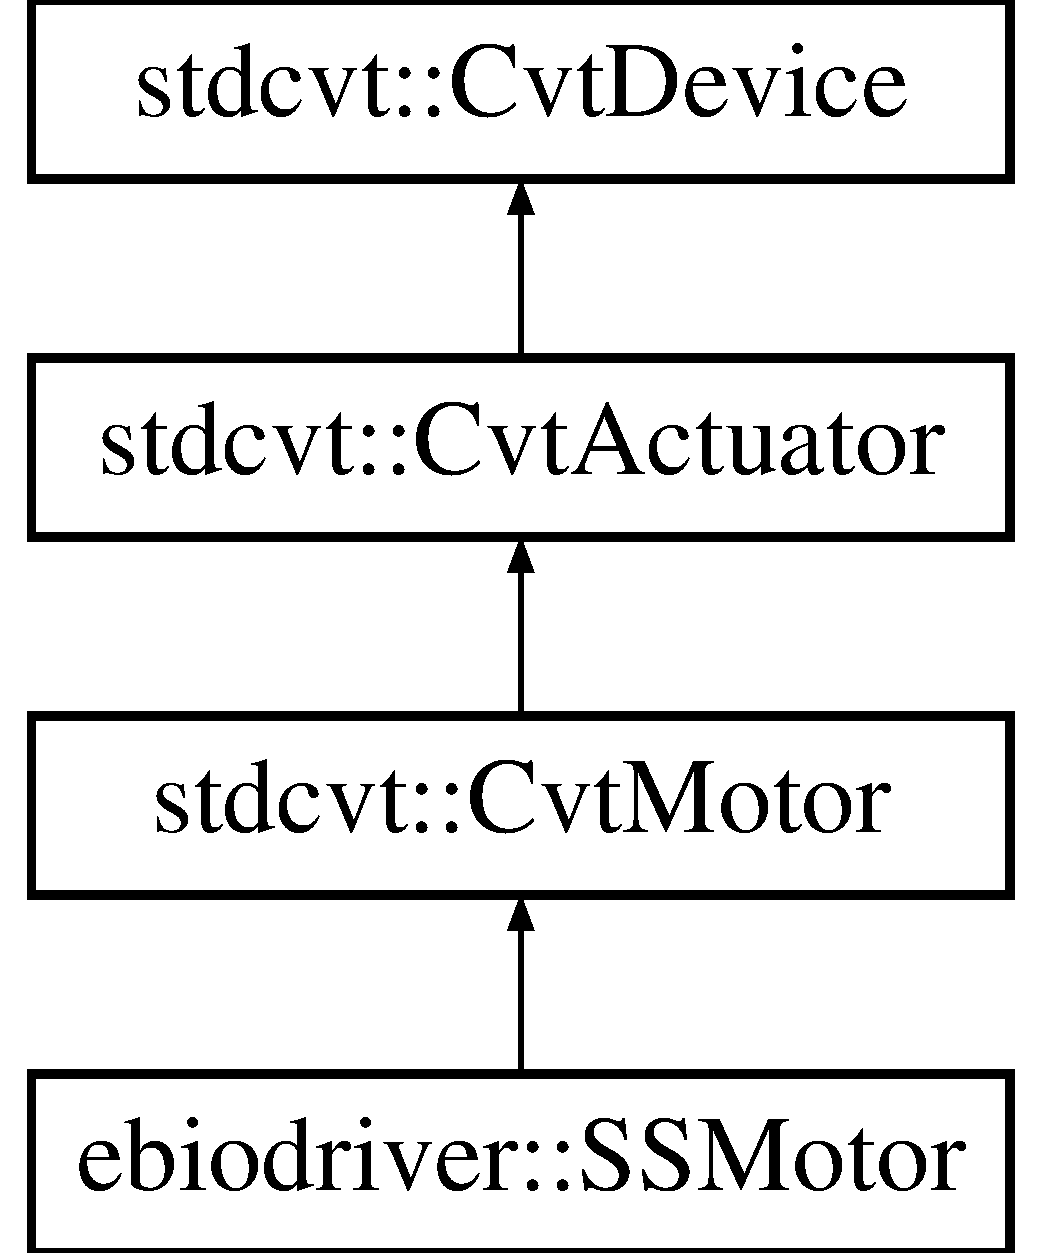
\includegraphics[height=4.000000cm]{classebiodriver_1_1SSMotor}
\end{center}
\end{figure}
\subsection*{Public 멤버 함수}
\begin{DoxyCompactItemize}
\item 
{\bfseries S\+S\+Motor} (int devid, \hyperlink{cvtcode_8h_ae8e34073e35cef0bb47c7fa535fc638b}{stdcvt\+::devtype\+\_\+t} devtype, \hyperlink{cvtcode_8h_a268eebb73363e24b9e65fd51973bd9c0}{stdcvt\+::devsec\+\_\+t} section, \hyperlink{cvtcode_8h_a2b37fd5cc4d40c0b8c4b987c271e5ceb}{stdcvt\+::devtarget\+\_\+t} target, \hyperlink{cvtcode_8h_ad21cd565f839adc5b19a0993e7da7278}{stdcvt\+::devstat\+\_\+t} devstatus)\hypertarget{classebiodriver_1_1SSMotor_a49e940a10a2c2abada3707429824fff0}{}\label{classebiodriver_1_1SSMotor_a49e940a10a2c2abada3707429824fff0}

\end{DoxyCompactItemize}
\subsection*{추가로 상속된 멤버들}


이 클래스에 대한 문서화 페이지는 다음의 파일로부터 생성되었습니다.\+:\begin{DoxyCompactItemize}
\item 
sample/\hyperlink{sssampledriver_8cpp}{sssampledriver.\+cpp}\end{DoxyCompactItemize}

\hypertarget{classebiodriver_1_1SSSampleDriver}{}\section{ebiodriver\+:\+:S\+S\+Sample\+Driver 클래스 참조}
\label{classebiodriver_1_1SSSampleDriver}\index{ebiodriver\+::\+S\+S\+Sample\+Driver@{ebiodriver\+::\+S\+S\+Sample\+Driver}}
ebiodriver\+:\+:S\+S\+Sample\+Driver에 대한 상속 다이어그램 \+: \begin{figure}[H]
\begin{center}
\leavevmode
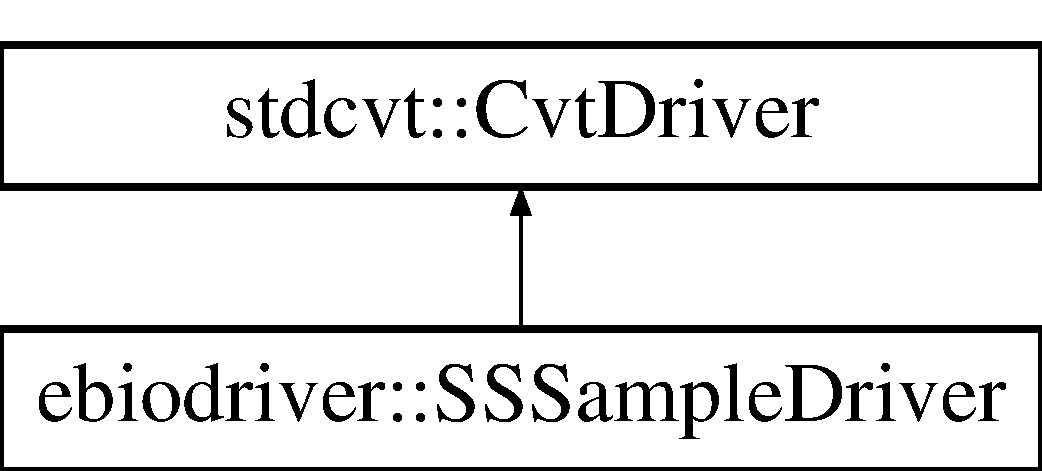
\includegraphics[height=2.000000cm]{classebiodriver_1_1SSSampleDriver}
\end{center}
\end{figure}
\subsection*{Public 멤버 함수}
\begin{DoxyCompactItemize}
\item 
\hyperlink{classebiodriver_1_1SSSampleDriver_afac6e5429ff3a9550925c1f62074ff3e}{S\+S\+Sample\+Driver} ()
\item 
const char $\ast$ \hyperlink{classebiodriver_1_1SSSampleDriver_a63d048b6c45e48bfc8f27e6a000a17fb}{getversion} ()
\item 
const char $\ast$ \hyperlink{classebiodriver_1_1SSSampleDriver_ac901fe0974866f1fa494b0bad342c562}{getmodel} ()
\item 
const char $\ast$ \hyperlink{classebiodriver_1_1SSSampleDriver_a34f317b0b97ad61cb6b9efe0f1920e21}{getcompany} ()
\item 
bool \hyperlink{classebiodriver_1_1SSSampleDriver_a604f906153e106692bd5869c7fd8888f}{initialize} (\hyperlink{classstdcvt_1_1CvtOption}{Cvt\+Option} option)
\item 
bool \hyperlink{classebiodriver_1_1SSSampleDriver_a43ab28051c128755cbb639d1c2db7ab2}{finalize} ()
\item 
bool \hyperlink{classebiodriver_1_1SSSampleDriver_a39622e2a63b609136d5e6740a329d450}{preprocess} ()
\item 
bool \hyperlink{classebiodriver_1_1SSSampleDriver_aa6dc852c3a6f9f5798a4ad53db7efbe3}{postprocess} ()
\item 
\hyperlink{classstdcvt_1_1CvtDevice}{Cvt\+Device} $\ast$ \hyperlink{classebiodriver_1_1SSSampleDriver_af4bdb5522559606b177416ec408cd4b4}{getdevice} (int index)
\item 
bool \hyperlink{classebiodriver_1_1SSSampleDriver_a268e69de75c71df87c32ad3d4aa29a91}{sharedevice} (\hyperlink{classstdcvt_1_1CvtDevice}{Cvt\+Device} $\ast$pdevice)
\item 
\hyperlink{classstdcvt_1_1CvtCommand}{Cvt\+Command} $\ast$ \hyperlink{classebiodriver_1_1SSSampleDriver_a273a5a2d7a1b54ba4d6d3989db78d152}{getcommand} (int index)
\item 
bool \hyperlink{classebiodriver_1_1SSSampleDriver_a25e63484cfbe11d3bc741c1cad5b240c}{control} (\hyperlink{classstdcvt_1_1CvtCommand}{Cvt\+Command} $\ast$pcmd)
\end{DoxyCompactItemize}


\subsection{생성자 \& 소멸자 문서화}
\index{ebiodriver\+::\+S\+S\+Sample\+Driver@{ebiodriver\+::\+S\+S\+Sample\+Driver}!S\+S\+Sample\+Driver@{S\+S\+Sample\+Driver}}
\index{S\+S\+Sample\+Driver@{S\+S\+Sample\+Driver}!ebiodriver\+::\+S\+S\+Sample\+Driver@{ebiodriver\+::\+S\+S\+Sample\+Driver}}
\subsubsection[{\texorpdfstring{S\+S\+Sample\+Driver()}{SSSampleDriver()}}]{\setlength{\rightskip}{0pt plus 5cm}ebiodriver\+::\+S\+S\+Sample\+Driver\+::\+S\+S\+Sample\+Driver (
\begin{DoxyParamCaption}
{}
\end{DoxyParamCaption}
)\hspace{0.3cm}{\ttfamily [inline]}}\hypertarget{classebiodriver_1_1SSSampleDriver_afac6e5429ff3a9550925c1f62074ff3e}{}\label{classebiodriver_1_1SSSampleDriver_afac6e5429ff3a9550925c1f62074ff3e}
새로운 D\+S드라이버를 생성한다. 
\begin{DoxyParams}{매개변수}
{\em modelcode} & 모델코드 \\
\hline
{\em apispec} & A\+PI 버전 \\
\hline
\end{DoxyParams}


\subsection{멤버 함수 문서화}
\index{ebiodriver\+::\+S\+S\+Sample\+Driver@{ebiodriver\+::\+S\+S\+Sample\+Driver}!control@{control}}
\index{control@{control}!ebiodriver\+::\+S\+S\+Sample\+Driver@{ebiodriver\+::\+S\+S\+Sample\+Driver}}
\subsubsection[{\texorpdfstring{control(\+Cvt\+Command $\ast$pcmd)}{control(CvtCommand *pcmd)}}]{\setlength{\rightskip}{0pt plus 5cm}bool ebiodriver\+::\+S\+S\+Sample\+Driver\+::control (
\begin{DoxyParamCaption}
\item[{{\bf Cvt\+Command} $\ast$}]{pcmd}
\end{DoxyParamCaption}
)\hspace{0.3cm}{\ttfamily [inline]}, {\ttfamily [virtual]}}\hypertarget{classebiodriver_1_1SSSampleDriver_a25e63484cfbe11d3bc741c1cad5b240c}{}\label{classebiodriver_1_1SSSampleDriver_a25e63484cfbe11d3bc741c1cad5b240c}
다른 드라이버로부터 명령을 받아 처리한다. 
\begin{DoxyParams}{매개변수}
{\em pcmd} & 명령에 대한 포인터 \\
\hline
\end{DoxyParams}
\begin{DoxyReturn}{반환값}
실제 명령의 처리 여부가 아니라 명령을 수신했는지 여부이다. 해당 명령을 실행할 장비가 없다면 false이다. 
\end{DoxyReturn}


\hyperlink{classstdcvt_1_1CvtDriver_ac289321a67d660f5514c4ddfaa238ade}{stdcvt\+::\+Cvt\+Driver}를 구현.

\index{ebiodriver\+::\+S\+S\+Sample\+Driver@{ebiodriver\+::\+S\+S\+Sample\+Driver}!finalize@{finalize}}
\index{finalize@{finalize}!ebiodriver\+::\+S\+S\+Sample\+Driver@{ebiodriver\+::\+S\+S\+Sample\+Driver}}
\subsubsection[{\texorpdfstring{finalize()}{finalize()}}]{\setlength{\rightskip}{0pt plus 5cm}bool ebiodriver\+::\+S\+S\+Sample\+Driver\+::finalize (
\begin{DoxyParamCaption}
{}
\end{DoxyParamCaption}
)\hspace{0.3cm}{\ttfamily [inline]}, {\ttfamily [virtual]}}\hypertarget{classebiodriver_1_1SSSampleDriver_a43ab28051c128755cbb639d1c2db7ab2}{}\label{classebiodriver_1_1SSSampleDriver_a43ab28051c128755cbb639d1c2db7ab2}
드라이버를 종료한다. \begin{DoxyReturn}{반환값}
종료 성공 여부 
\end{DoxyReturn}


\hyperlink{classstdcvt_1_1CvtDriver_a22b39da5aafabec2ee9677ed138256e9}{stdcvt\+::\+Cvt\+Driver}를 구현.

\index{ebiodriver\+::\+S\+S\+Sample\+Driver@{ebiodriver\+::\+S\+S\+Sample\+Driver}!getcommand@{getcommand}}
\index{getcommand@{getcommand}!ebiodriver\+::\+S\+S\+Sample\+Driver@{ebiodriver\+::\+S\+S\+Sample\+Driver}}
\subsubsection[{\texorpdfstring{getcommand(int index)}{getcommand(int index)}}]{\setlength{\rightskip}{0pt plus 5cm}{\bf Cvt\+Command}$\ast$ ebiodriver\+::\+S\+S\+Sample\+Driver\+::getcommand (
\begin{DoxyParamCaption}
\item[{int}]{index}
\end{DoxyParamCaption}
)\hspace{0.3cm}{\ttfamily [inline]}, {\ttfamily [virtual]}}\hypertarget{classebiodriver_1_1SSSampleDriver_a273a5a2d7a1b54ba4d6d3989db78d152}{}\label{classebiodriver_1_1SSSampleDriver_a273a5a2d7a1b54ba4d6d3989db78d152}
다른 드라이버가 관리하고 있는 장비를 제어하고자 할때 명령을 전달한다. 명령을 전달하지 않는 드라이버라면 그냥 N\+U\+L\+L을 리턴하도록 만들면 된다. 
\begin{DoxyParams}{매개변수}
{\em index} & 얻고자 하는 명령의 인덱스 번호. 0에서 시작한다. \\
\hline
\end{DoxyParams}
\begin{DoxyReturn}{반환값}
인덱스에 해당하는 명령의 포인터. N\+U\+LL 이라면 이후에 명령이 없다는 의미이다. 
\end{DoxyReturn}


\hyperlink{classstdcvt_1_1CvtDriver_ad0378635152f2e35c0686c4fe92996e6}{stdcvt\+::\+Cvt\+Driver}를 구현.

\index{ebiodriver\+::\+S\+S\+Sample\+Driver@{ebiodriver\+::\+S\+S\+Sample\+Driver}!getcompany@{getcompany}}
\index{getcompany@{getcompany}!ebiodriver\+::\+S\+S\+Sample\+Driver@{ebiodriver\+::\+S\+S\+Sample\+Driver}}
\subsubsection[{\texorpdfstring{getcompany()}{getcompany()}}]{\setlength{\rightskip}{0pt plus 5cm}const char$\ast$ ebiodriver\+::\+S\+S\+Sample\+Driver\+::getcompany (
\begin{DoxyParamCaption}
{}
\end{DoxyParamCaption}
)\hspace{0.3cm}{\ttfamily [inline]}, {\ttfamily [virtual]}}\hypertarget{classebiodriver_1_1SSSampleDriver_a34f317b0b97ad61cb6b9efe0f1920e21}{}\label{classebiodriver_1_1SSSampleDriver_a34f317b0b97ad61cb6b9efe0f1920e21}
드라이버 제조사명을 확인한다. 컨버터에서는 제조사명을 로깅용도로만 사용한다. \begin{DoxyReturn}{반환값}
문자열 형식의 제조사명 
\end{DoxyReturn}


\hyperlink{classstdcvt_1_1CvtDriver_af77365bd31120078fa2eae4ddece3028}{stdcvt\+::\+Cvt\+Driver}를 구현.

\index{ebiodriver\+::\+S\+S\+Sample\+Driver@{ebiodriver\+::\+S\+S\+Sample\+Driver}!getdevice@{getdevice}}
\index{getdevice@{getdevice}!ebiodriver\+::\+S\+S\+Sample\+Driver@{ebiodriver\+::\+S\+S\+Sample\+Driver}}
\subsubsection[{\texorpdfstring{getdevice(int index)}{getdevice(int index)}}]{\setlength{\rightskip}{0pt plus 5cm}{\bf Cvt\+Device}$\ast$ ebiodriver\+::\+S\+S\+Sample\+Driver\+::getdevice (
\begin{DoxyParamCaption}
\item[{int}]{index}
\end{DoxyParamCaption}
)\hspace{0.3cm}{\ttfamily [inline]}, {\ttfamily [virtual]}}\hypertarget{classebiodriver_1_1SSSampleDriver_af4bdb5522559606b177416ec408cd4b4}{}\label{classebiodriver_1_1SSSampleDriver_af4bdb5522559606b177416ec408cd4b4}
드라이버가 관리하고 있는 장비의 포인터를 꺼내준다. 
\begin{DoxyParams}{매개변수}
{\em index} & 얻고자 하는 장비의 인덱스 번호. 0에서 시작한다. \\
\hline
\end{DoxyParams}
\begin{DoxyReturn}{반환값}
인덱스에 해당하는 장비의 포인터. N\+U\+LL 이라면 이후에 장비가 없다는 의미이다. 
\end{DoxyReturn}


\hyperlink{classstdcvt_1_1CvtDriver_adc2ce5ff6fe2426fd84ce3ae69731704}{stdcvt\+::\+Cvt\+Driver}를 구현.

\index{ebiodriver\+::\+S\+S\+Sample\+Driver@{ebiodriver\+::\+S\+S\+Sample\+Driver}!getmodel@{getmodel}}
\index{getmodel@{getmodel}!ebiodriver\+::\+S\+S\+Sample\+Driver@{ebiodriver\+::\+S\+S\+Sample\+Driver}}
\subsubsection[{\texorpdfstring{getmodel()}{getmodel()}}]{\setlength{\rightskip}{0pt plus 5cm}const char$\ast$ ebiodriver\+::\+S\+S\+Sample\+Driver\+::getmodel (
\begin{DoxyParamCaption}
{}
\end{DoxyParamCaption}
)\hspace{0.3cm}{\ttfamily [inline]}, {\ttfamily [virtual]}}\hypertarget{classebiodriver_1_1SSSampleDriver_ac901fe0974866f1fa494b0bad342c562}{}\label{classebiodriver_1_1SSSampleDriver_ac901fe0974866f1fa494b0bad342c562}
드라이버 제작자가 부여하는 모델번호를 확인한다. \begin{DoxyReturn}{반환값}
문자열 형식의 모델번호 
\end{DoxyReturn}


\hyperlink{classstdcvt_1_1CvtDriver_a384233eb993e566102cbcc5e87db3e96}{stdcvt\+::\+Cvt\+Driver}를 구현.

\index{ebiodriver\+::\+S\+S\+Sample\+Driver@{ebiodriver\+::\+S\+S\+Sample\+Driver}!getversion@{getversion}}
\index{getversion@{getversion}!ebiodriver\+::\+S\+S\+Sample\+Driver@{ebiodriver\+::\+S\+S\+Sample\+Driver}}
\subsubsection[{\texorpdfstring{getversion()}{getversion()}}]{\setlength{\rightskip}{0pt plus 5cm}const char$\ast$ ebiodriver\+::\+S\+S\+Sample\+Driver\+::getversion (
\begin{DoxyParamCaption}
{}
\end{DoxyParamCaption}
)\hspace{0.3cm}{\ttfamily [inline]}, {\ttfamily [virtual]}}\hypertarget{classebiodriver_1_1SSSampleDriver_a63d048b6c45e48bfc8f27e6a000a17fb}{}\label{classebiodriver_1_1SSSampleDriver_a63d048b6c45e48bfc8f27e6a000a17fb}
드라이버 제작자가 부여하는 버전번호를 확인한다. \begin{DoxyReturn}{반환값}
문자열 형식의 버전번호 
\end{DoxyReturn}


\hyperlink{classstdcvt_1_1CvtDriver_a8c813cb2be4b0f3bb02c99125488ac24}{stdcvt\+::\+Cvt\+Driver}를 구현.

\index{ebiodriver\+::\+S\+S\+Sample\+Driver@{ebiodriver\+::\+S\+S\+Sample\+Driver}!initialize@{initialize}}
\index{initialize@{initialize}!ebiodriver\+::\+S\+S\+Sample\+Driver@{ebiodriver\+::\+S\+S\+Sample\+Driver}}
\subsubsection[{\texorpdfstring{initialize(\+Cvt\+Option option)}{initialize(CvtOption option)}}]{\setlength{\rightskip}{0pt plus 5cm}bool ebiodriver\+::\+S\+S\+Sample\+Driver\+::initialize (
\begin{DoxyParamCaption}
\item[{{\bf Cvt\+Option}}]{option}
\end{DoxyParamCaption}
)\hspace{0.3cm}{\ttfamily [inline]}, {\ttfamily [virtual]}}\hypertarget{classebiodriver_1_1SSSampleDriver_a604f906153e106692bd5869c7fd8888f}{}\label{classebiodriver_1_1SSSampleDriver_a604f906153e106692bd5869c7fd8888f}
드라이버를 초기화 한다. 드라이버 동작을 위한 option 은 key-\/value 형식으로 전달된다. 
\begin{DoxyParams}{매개변수}
{\em option} & 드라이버동작을 위한 옵션 \\
\hline
\end{DoxyParams}
\begin{DoxyReturn}{반환값}
초기화 성공 여부 
\end{DoxyReturn}


\hyperlink{classstdcvt_1_1CvtDriver_a71322934c5b5ad0d5b167219cd23a0bb}{stdcvt\+::\+Cvt\+Driver}를 구현.

\index{ebiodriver\+::\+S\+S\+Sample\+Driver@{ebiodriver\+::\+S\+S\+Sample\+Driver}!postprocess@{postprocess}}
\index{postprocess@{postprocess}!ebiodriver\+::\+S\+S\+Sample\+Driver@{ebiodriver\+::\+S\+S\+Sample\+Driver}}
\subsubsection[{\texorpdfstring{postprocess()}{postprocess()}}]{\setlength{\rightskip}{0pt plus 5cm}bool ebiodriver\+::\+S\+S\+Sample\+Driver\+::postprocess (
\begin{DoxyParamCaption}
{}
\end{DoxyParamCaption}
)\hspace{0.3cm}{\ttfamily [inline]}, {\ttfamily [virtual]}}\hypertarget{classebiodriver_1_1SSSampleDriver_aa6dc852c3a6f9f5798a4ad53db7efbe3}{}\label{classebiodriver_1_1SSSampleDriver_aa6dc852c3a6f9f5798a4ad53db7efbe3}
드라이버간 상태교환이 이루어진 이후에 호출되는 메소드로 후처리를 수행한다. \begin{DoxyReturn}{반환값}
후처리 성공 여부 
\end{DoxyReturn}


\hyperlink{classstdcvt_1_1CvtDriver_a4bcae9e7c58d989a645a74d21e2fc5ea}{stdcvt\+::\+Cvt\+Driver}를 구현.

\index{ebiodriver\+::\+S\+S\+Sample\+Driver@{ebiodriver\+::\+S\+S\+Sample\+Driver}!preprocess@{preprocess}}
\index{preprocess@{preprocess}!ebiodriver\+::\+S\+S\+Sample\+Driver@{ebiodriver\+::\+S\+S\+Sample\+Driver}}
\subsubsection[{\texorpdfstring{preprocess()}{preprocess()}}]{\setlength{\rightskip}{0pt plus 5cm}bool ebiodriver\+::\+S\+S\+Sample\+Driver\+::preprocess (
\begin{DoxyParamCaption}
{}
\end{DoxyParamCaption}
)\hspace{0.3cm}{\ttfamily [inline]}, {\ttfamily [virtual]}}\hypertarget{classebiodriver_1_1SSSampleDriver_a39622e2a63b609136d5e6740a329d450}{}\label{classebiodriver_1_1SSSampleDriver_a39622e2a63b609136d5e6740a329d450}
드라이버간 상태교환을 하기전에 호출되는 메소드로 전처리를 수행한다. \begin{DoxyReturn}{반환값}
전처리 성공 여부 
\end{DoxyReturn}


\hyperlink{classstdcvt_1_1CvtDriver_ac15259a26d652d46c198307886d52257}{stdcvt\+::\+Cvt\+Driver}를 구현.

\index{ebiodriver\+::\+S\+S\+Sample\+Driver@{ebiodriver\+::\+S\+S\+Sample\+Driver}!sharedevice@{sharedevice}}
\index{sharedevice@{sharedevice}!ebiodriver\+::\+S\+S\+Sample\+Driver@{ebiodriver\+::\+S\+S\+Sample\+Driver}}
\subsubsection[{\texorpdfstring{sharedevice(\+Cvt\+Device $\ast$pdevice)}{sharedevice(CvtDevice *pdevice)}}]{\setlength{\rightskip}{0pt plus 5cm}bool ebiodriver\+::\+S\+S\+Sample\+Driver\+::sharedevice (
\begin{DoxyParamCaption}
\item[{{\bf Cvt\+Device} $\ast$}]{pdevice}
\end{DoxyParamCaption}
)\hspace{0.3cm}{\ttfamily [inline]}, {\ttfamily [virtual]}}\hypertarget{classebiodriver_1_1SSSampleDriver_a268e69de75c71df87c32ad3d4aa29a91}{}\label{classebiodriver_1_1SSSampleDriver_a268e69de75c71df87c32ad3d4aa29a91}
전달된 장비의 정보를 획득한다. 다른 드라이버의 장비정보를 입력해주기 위해 컨버터가 호출한다. 
\begin{DoxyParams}{매개변수}
{\em pdevice} & 다른 드라이버의 장비 포인터 \\
\hline
\end{DoxyParams}
\begin{DoxyReturn}{반환값}
성공여부. 관심이 없는 장비인 경우라도 문제가 없으면 true를 리턴한다. 
\end{DoxyReturn}


\hyperlink{classstdcvt_1_1CvtDriver_aeedcd62d3b6ed95f0584db5a7259f642}{stdcvt\+::\+Cvt\+Driver}를 구현.



이 클래스에 대한 문서화 페이지는 다음의 파일로부터 생성되었습니다.\+:\begin{DoxyCompactItemize}
\item 
sample/\hyperlink{sssampledriver_8cpp}{sssampledriver.\+cpp}\end{DoxyCompactItemize}

\hypertarget{classebiodriver_1_1SSSensor}{}\section{ebiodriver\+:\+:S\+S\+Sensor 클래스 참조}
\label{classebiodriver_1_1SSSensor}\index{ebiodriver\+::\+S\+S\+Sensor@{ebiodriver\+::\+S\+S\+Sensor}}
ebiodriver\+:\+:S\+S\+Sensor에 대한 상속 다이어그램 \+: \begin{figure}[H]
\begin{center}
\leavevmode
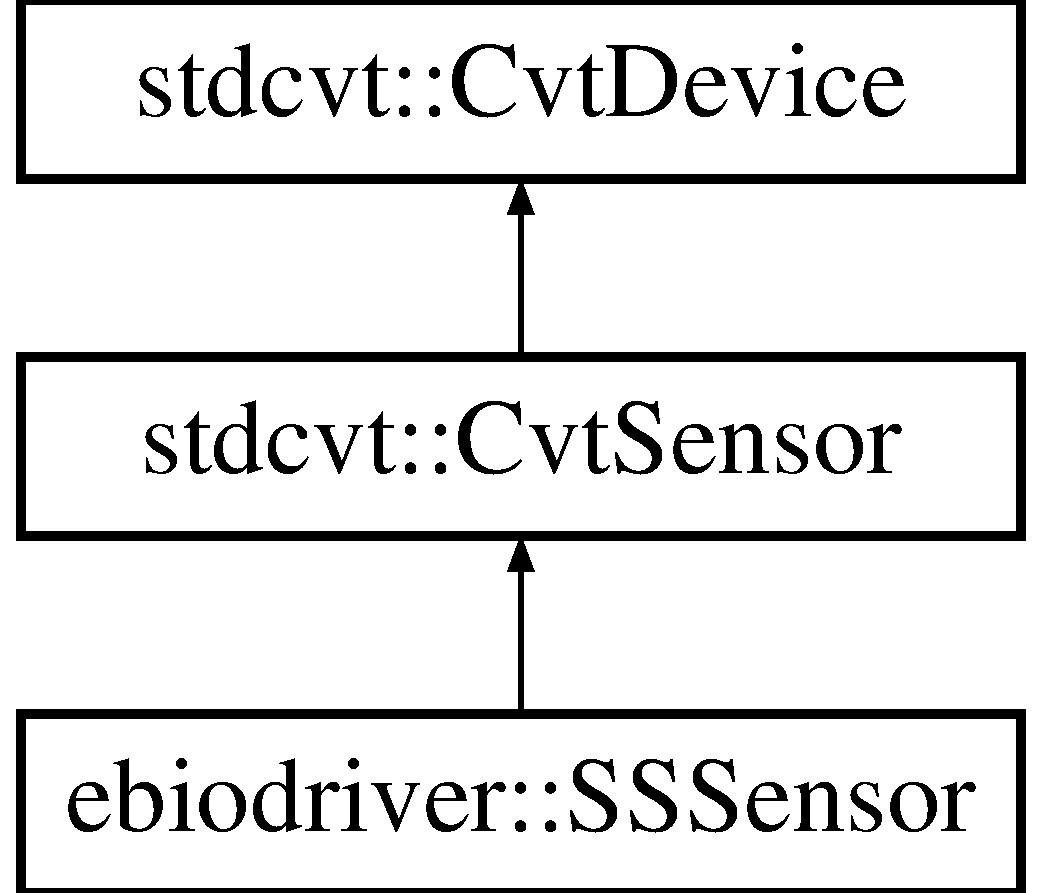
\includegraphics[height=3.000000cm]{classebiodriver_1_1SSSensor}
\end{center}
\end{figure}
\subsection*{Public 멤버 함수}
\begin{DoxyCompactItemize}
\item 
{\bfseries S\+S\+Sensor} (int devid, \hyperlink{cvtcode_8h_ae8e34073e35cef0bb47c7fa535fc638b}{stdcvt\+::devtype\+\_\+t} devtype, \hyperlink{cvtcode_8h_a268eebb73363e24b9e65fd51973bd9c0}{stdcvt\+::devsec\+\_\+t} section, \hyperlink{cvtcode_8h_a2b37fd5cc4d40c0b8c4b987c271e5ceb}{stdcvt\+::devtarget\+\_\+t} target, \hyperlink{cvtcode_8h_ad21cd565f839adc5b19a0993e7da7278}{stdcvt\+::devstat\+\_\+t} devstatus, \hyperlink{cvtcode_8h_a6d4ed81d95144c5eedcd08eda1e800a4}{stdcvt\+::obsunit\+\_\+t} unit)\hypertarget{classebiodriver_1_1SSSensor_aa1fef3c59c8d1ef97426b18ee10fa1ea}{}\label{classebiodriver_1_1SSSensor_aa1fef3c59c8d1ef97426b18ee10fa1ea}

\end{DoxyCompactItemize}


이 클래스에 대한 문서화 페이지는 다음의 파일로부터 생성되었습니다.\+:\begin{DoxyCompactItemize}
\item 
sample/\hyperlink{sssampledriver_8cpp}{sssampledriver.\+cpp}\end{DoxyCompactItemize}

\hypertarget{classebiodriver_1_1SSSwitch}{}\section{ebiodriver\+:\+:S\+S\+Switch 클래스 참조}
\label{classebiodriver_1_1SSSwitch}\index{ebiodriver\+::\+S\+S\+Switch@{ebiodriver\+::\+S\+S\+Switch}}
ebiodriver\+:\+:S\+S\+Switch에 대한 상속 다이어그램 \+: \begin{figure}[H]
\begin{center}
\leavevmode
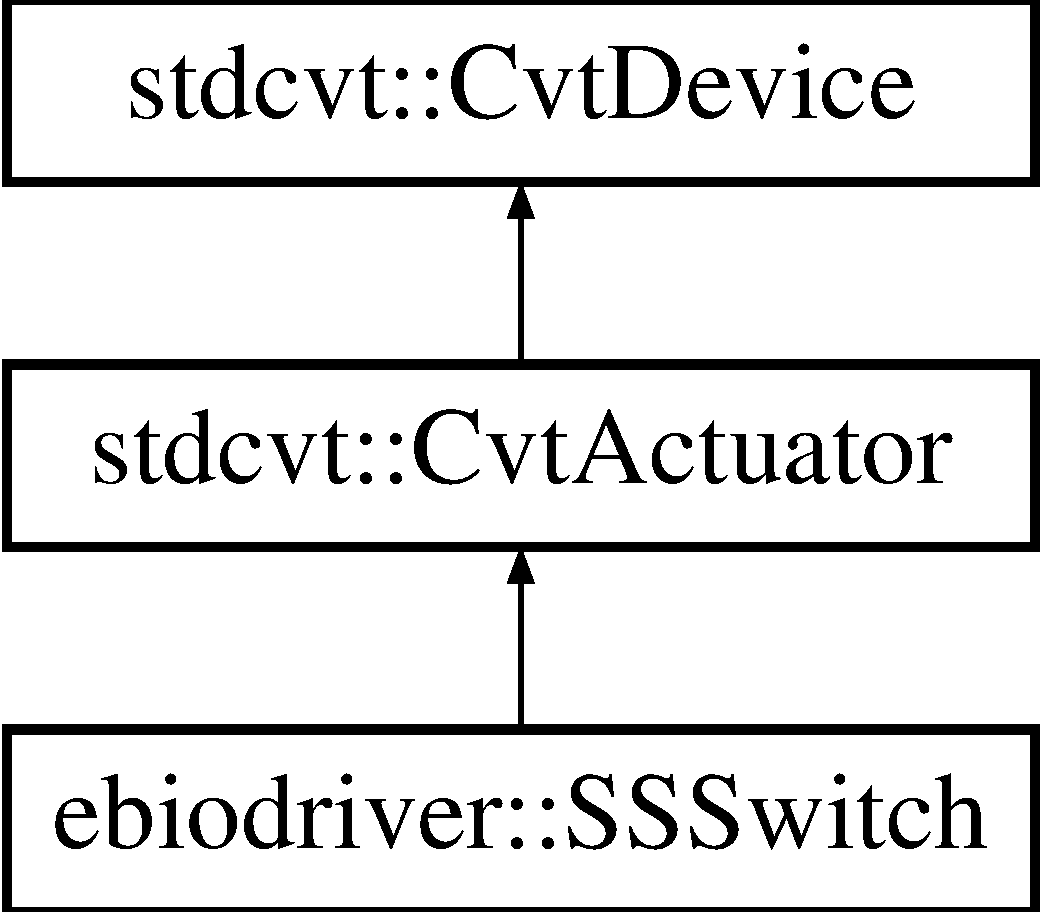
\includegraphics[height=3.000000cm]{classebiodriver_1_1SSSwitch}
\end{center}
\end{figure}
\subsection*{Public 멤버 함수}
\begin{DoxyCompactItemize}
\item 
{\bfseries S\+S\+Switch} (int devid, \hyperlink{cvtcode_8h_ae8e34073e35cef0bb47c7fa535fc638b}{stdcvt\+::devtype\+\_\+t} devtype, \hyperlink{cvtcode_8h_a268eebb73363e24b9e65fd51973bd9c0}{stdcvt\+::devsec\+\_\+t} section, \hyperlink{cvtcode_8h_a2b37fd5cc4d40c0b8c4b987c271e5ceb}{stdcvt\+::devtarget\+\_\+t} target, \hyperlink{cvtcode_8h_ad21cd565f839adc5b19a0993e7da7278}{stdcvt\+::devstat\+\_\+t} devstatus)\hypertarget{classebiodriver_1_1SSSwitch_a9c034c81460c009e7d97138b43ee1e2e}{}\label{classebiodriver_1_1SSSwitch_a9c034c81460c009e7d97138b43ee1e2e}

\end{DoxyCompactItemize}
\subsection*{추가로 상속된 멤버들}


이 클래스에 대한 문서화 페이지는 다음의 파일로부터 생성되었습니다.\+:\begin{DoxyCompactItemize}
\item 
sample/\hyperlink{sssampledriver_8cpp}{sssampledriver.\+cpp}\end{DoxyCompactItemize}

\chapter{파일 문서화}
\hypertarget{dssampledriver_8cpp}{}\section{sample/dssampledriver.cpp 파일 참조}
\label{dssampledriver_8cpp}\index{sample/dssampledriver.\+cpp@{sample/dssampledriver.\+cpp}}
{\ttfamily \#include $<$iostream$>$}\\*
{\ttfamily \#include $<$sstream$>$}\\*
{\ttfamily \#include $<$string$>$}\\*
{\ttfamily \#include $<$boost/asio.\+hpp$>$}\\*
{\ttfamily \#include $<$boost/bind.\+hpp$>$}\\*
{\ttfamily \#include $<$boost/config.\+hpp$>$}\\*
{\ttfamily \#include $<$glog/logging.\+h$>$}\\*
{\ttfamily \#include \char`\"{}../spec/cvtdriver.\+h\char`\"{}}\\*
\subsection*{데이타 구조}
\begin{DoxyCompactItemize}
\item 
class \hyperlink{classebiodriver_1_1DSSampleDriver}{ebiodriver\+::\+D\+S\+Sample\+Driver}
\end{DoxyCompactItemize}
\subsection*{매크로}
\begin{DoxyCompactItemize}
\item 
\#define {\bfseries B\+U\+F\+S\+I\+ZE}~128\hypertarget{dssampledriver_8cpp_aeca034f67218340ecb2261a22c2f3dcd}{}\label{dssampledriver_8cpp_aeca034f67218340ecb2261a22c2f3dcd}

\item 
\#define {\bfseries S\+M\+A\+RK}~\textquotesingle{}$^\wedge$\textquotesingle{}\hypertarget{dssampledriver_8cpp_aab8d124dc1be2d0d447869b79f6d8513}{}\label{dssampledriver_8cpp_aab8d124dc1be2d0d447869b79f6d8513}

\item 
\#define {\bfseries E\+M\+A\+RK}~\textquotesingle{}\$\textquotesingle{}\hypertarget{dssampledriver_8cpp_affd7eab8a44edfe61450f2c02715e368}{}\label{dssampledriver_8cpp_affd7eab8a44edfe61450f2c02715e368}

\end{DoxyCompactItemize}
\subsection*{변수}
\begin{DoxyCompactItemize}
\item 
B\+O\+O\+S\+T\+\_\+\+S\+Y\+M\+B\+O\+L\+\_\+\+E\+X\+P\+O\+RT D\+S\+Sample\+Driver {\bfseries ebiodriver\+::plugin}\hypertarget{dssampledriver_8cpp_a09ecfae3744bdd4bd2cffa770b192f4c}{}\label{dssampledriver_8cpp_a09ecfae3744bdd4bd2cffa770b192f4c}

\end{DoxyCompactItemize}


\subsection{상세한 설명}
Copyright © 2018 ebio lab. S\+NU. All Rights Reserved.

\begin{DoxyDate}{날짜}
2018-\/02-\/27, Joon\+Yong 
\end{DoxyDate}
\begin{DoxyAuthor}{작성자}
Kim, Joon\+Yong \href{mailto:tombraid@snu.ac.kr}{\tt tombraid@snu.\+ac.\+kr}
\end{DoxyAuthor}
This file is for sample driver. refer from\+: \href{https://github.com/ebio-snu/cvtdriver}{\tt https\+://github.\+com/ebio-\/snu/cvtdriver} 
\hypertarget{sssampledriver_8cpp}{}\section{sample/sssampledriver.cpp 파일 참조}
\label{sssampledriver_8cpp}\index{sample/sssampledriver.\+cpp@{sample/sssampledriver.\+cpp}}
{\ttfamily \#include $<$iostream$>$}\\*
{\ttfamily \#include $<$sstream$>$}\\*
{\ttfamily \#include $<$string$>$}\\*
{\ttfamily \#include $<$boost/config.\+hpp$>$}\\*
{\ttfamily \#include $<$glog/logging.\+h$>$}\\*
{\ttfamily \#include \char`\"{}../spec/cvtdevice.\+h\char`\"{}}\\*
{\ttfamily \#include \char`\"{}../spec/cvtdriver.\+h\char`\"{}}\\*
\subsection*{데이타 구조}
\begin{DoxyCompactItemize}
\item 
class \hyperlink{classebiodriver_1_1SSSensor}{ebiodriver\+::\+S\+S\+Sensor}
\item 
class \hyperlink{classebiodriver_1_1SSMotor}{ebiodriver\+::\+S\+S\+Motor}
\item 
class \hyperlink{classebiodriver_1_1SSSwitch}{ebiodriver\+::\+S\+S\+Switch}
\item 
class \hyperlink{classebiodriver_1_1SSSampleDriver}{ebiodriver\+::\+S\+S\+Sample\+Driver}
\end{DoxyCompactItemize}
\subsection*{매크로}
\begin{DoxyCompactItemize}
\item 
\#define {\bfseries B\+U\+F\+S\+I\+ZE}~128\hypertarget{sssampledriver_8cpp_aeca034f67218340ecb2261a22c2f3dcd}{}\label{sssampledriver_8cpp_aeca034f67218340ecb2261a22c2f3dcd}

\end{DoxyCompactItemize}


\subsection{상세한 설명}
Copyright © 2018 ebio lab. S\+NU. All Rights Reserved.

\begin{DoxyDate}{날짜}
2018-\/02-\/27, Joon\+Yong 
\end{DoxyDate}
\begin{DoxyAuthor}{작성자}
Kim, Joon\+Yong \href{mailto:tombraid@snu.ac.kr}{\tt tombraid@snu.\+ac.\+kr}
\end{DoxyAuthor}
This file is for sample driver. refer from\+: \href{https://github.com/ebio-snu/cvtdriver}{\tt https\+://github.\+com/ebio-\/snu/cvtdriver} 
\hypertarget{cvtcode_8h}{}\section{spec/cvtcode.h 파일 참조}
\label{cvtcode_8h}\index{spec/cvtcode.\+h@{spec/cvtcode.\+h}}
\subsection*{매크로}
\begin{DoxyCompactItemize}
\item 
\#define \hyperlink{cvtcode_8h_a7289fda70ed3a9989d210c5401227d33}{C\+V\+T\+\_\+\+O\+P\+T\+I\+O\+N\+\_\+\+A\+S\+I\+O\+\_\+\+S\+E\+R\+V\+I\+CE}~\char`\"{}opt\+\_\+asio\+\_\+service\char`\"{}\hypertarget{cvtcode_8h_a7289fda70ed3a9989d210c5401227d33}{}\label{cvtcode_8h_a7289fda70ed3a9989d210c5401227d33}

\begin{DoxyCompactList}\small\item\em boost\+::asio\+::io\+\_\+service 를 위한 옵션 키 \end{DoxyCompactList}\item 
\#define \hyperlink{cvtcode_8h_a0a32c0c21a9ae887f5489d643b2cff88}{D\+L\+\_\+\+U\+N\+K\+N\+O\+WN}~-\/2\hypertarget{cvtcode_8h_a0a32c0c21a9ae887f5489d643b2cff88}{}\label{cvtcode_8h_a0a32c0c21a9ae887f5489d643b2cff88}

\begin{DoxyCompactList}\small\item\em 설치구역 알수 없음 \end{DoxyCompactList}\item 
\#define \hyperlink{cvtcode_8h_a6f6c163690735e1bbddd35bb30014484}{D\+L\+\_\+\+O\+U\+T\+S\+I\+DE}~-\/1\hypertarget{cvtcode_8h_a6f6c163690735e1bbddd35bb30014484}{}\label{cvtcode_8h_a6f6c163690735e1bbddd35bb30014484}

\begin{DoxyCompactList}\small\item\em 설치구역 외부 \end{DoxyCompactList}\item 
\#define \hyperlink{cvtcode_8h_ac6db925c0a4407f0950b9a8a57604b41}{D\+L\+\_\+\+D\+E\+F\+A\+U\+L\+T\+\_\+\+R\+O\+O\+T\+Z\+O\+NE}~10103010101\hypertarget{cvtcode_8h_ac6db925c0a4407f0950b9a8a57604b41}{}\label{cvtcode_8h_ac6db925c0a4407f0950b9a8a57604b41}

\begin{DoxyCompactList}\small\item\em 디폴트 설치구역 지하부 \end{DoxyCompactList}\item 
\#define \hyperlink{cvtcode_8h_abb7af65ed66bdda6afa7bc6b494db757}{D\+L\+\_\+\+D\+E\+F\+A\+U\+L\+T\+\_\+\+P\+L\+A\+N\+T\+Z\+O\+NE}~10103010102\hypertarget{cvtcode_8h_abb7af65ed66bdda6afa7bc6b494db757}{}\label{cvtcode_8h_abb7af65ed66bdda6afa7bc6b494db757}

\begin{DoxyCompactList}\small\item\em 디폴트 설치구역 작물부 \end{DoxyCompactList}\item 
\#define \hyperlink{cvtcode_8h_a7c06ee300eef05f7739db3ea81f2e52e}{D\+L\+\_\+\+D\+E\+F\+A\+U\+L\+T\+\_\+\+R\+O\+O\+F\+Z\+O\+NE}~10103010103\hypertarget{cvtcode_8h_a7c06ee300eef05f7739db3ea81f2e52e}{}\label{cvtcode_8h_a7c06ee300eef05f7739db3ea81f2e52e}

\begin{DoxyCompactList}\small\item\em 디폴드 설치구역 작물상부 \end{DoxyCompactList}\end{DoxyCompactItemize}
\subsection*{타입정의}
\begin{DoxyCompactItemize}
\item 
typedef long \hyperlink{cvtcode_8h_a268eebb73363e24b9e65fd51973bd9c0}{stdcvt\+::devsec\+\_\+t}
\end{DoxyCompactItemize}
\subsection*{열거형 타입}
\begin{DoxyCompactItemize}
\item 
enum \hyperlink{cvtcode_8h_ad21cd565f839adc5b19a0993e7da7278}{stdcvt\+::devstat\+\_\+t} \{ \\*
\hyperlink{cvtcode_8h_ad21cd565f839adc5b19a0993e7da7278ac96b672b451f37bf12a29fa813d15860}{stdcvt\+::\+D\+S\+\_\+\+D\+E\+V\+\_\+\+A\+B\+N\+O\+R\+M\+AL} = 1, 
\hyperlink{cvtcode_8h_ad21cd565f839adc5b19a0993e7da7278a1d8578630c15db41817c1becddac8ab0}{stdcvt\+::\+D\+S\+\_\+\+S\+E\+N\+\_\+\+N\+O\+R\+M\+AL} = 101, 
\hyperlink{cvtcode_8h_ad21cd565f839adc5b19a0993e7da7278a80b5bd9870b71f52a83f1a95fee8d817}{stdcvt\+::\+D\+S\+\_\+\+S\+W\+C\+\_\+\+ON} = 201, 
\hyperlink{cvtcode_8h_ad21cd565f839adc5b19a0993e7da7278a595b04d86677f3e27bf302ac021ecd89}{stdcvt\+::\+D\+S\+\_\+\+S\+W\+C\+\_\+\+O\+FF} = 202, 
\\*
\hyperlink{cvtcode_8h_ad21cd565f839adc5b19a0993e7da7278a7e9ee99206654bf0c371e48ea77819ad}{stdcvt\+::\+D\+S\+\_\+\+M\+O\+T\+\_\+\+O\+P\+EN} = 301, 
\hyperlink{cvtcode_8h_ad21cd565f839adc5b19a0993e7da7278aaa2b6a2fc2d613140c844f2493684512}{stdcvt\+::\+D\+S\+\_\+\+M\+O\+T\+\_\+\+C\+L\+O\+SE} = 302, 
\hyperlink{cvtcode_8h_ad21cd565f839adc5b19a0993e7da7278ab2a98aa7c4709840543847794e8ab535}{stdcvt\+::\+D\+S\+\_\+\+M\+O\+T\+\_\+\+S\+T\+OP} = 303
 \}
\item 
enum \hyperlink{cvtcode_8h_a2b37fd5cc4d40c0b8c4b987c271e5ceb}{stdcvt\+::devtarget\+\_\+t} \{ \\*
\hyperlink{cvtcode_8h_a2b37fd5cc4d40c0b8c4b987c271e5cebaa0e4886064d0936ecb24963d248587bc}{stdcvt\+::\+D\+O\+\_\+\+U\+N\+K\+N\+O\+WN} = 1, 
\hyperlink{cvtcode_8h_a2b37fd5cc4d40c0b8c4b987c271e5ceba3b49e7fda4269fc068dbbfe4a9f233a5}{stdcvt\+::\+D\+O\+\_\+\+E\+N\+V\+\_\+\+A\+T\+M\+O\+S\+P\+H\+E\+RE} = 1001, 
\hyperlink{cvtcode_8h_a2b37fd5cc4d40c0b8c4b987c271e5ceba585e93b280b1d4dcccd851f08fb7b8dd}{stdcvt\+::\+D\+O\+\_\+\+E\+N\+V\+\_\+\+S\+O\+IL} = 1002, 
\hyperlink{cvtcode_8h_a2b37fd5cc4d40c0b8c4b987c271e5cebaa26e34d2b75de2c762fe9eeaf04f35e4}{stdcvt\+::\+D\+O\+\_\+\+E\+N\+V\+\_\+\+N\+U\+T\+R\+I\+E\+N\+T\+S\+O\+L\+U\+T\+I\+ON} = 1003, 
\\*
\hyperlink{cvtcode_8h_a2b37fd5cc4d40c0b8c4b987c271e5ceba0fd181d2dc205f8dc1b5bd2f28fe2656}{stdcvt\+::\+D\+O\+\_\+\+P\+L\+A\+N\+T\+\_\+\+S\+T\+EM} = 2001, 
\hyperlink{cvtcode_8h_a2b37fd5cc4d40c0b8c4b987c271e5ceba29163db618d23c82f95ba5a3d7e76645}{stdcvt\+::\+D\+O\+\_\+\+P\+L\+A\+N\+T\+\_\+\+L\+E\+AF} = 2002, 
\hyperlink{cvtcode_8h_a2b37fd5cc4d40c0b8c4b987c271e5ceba8d31fadc17cb9bd4510fb0e1b1999920}{stdcvt\+::\+D\+O\+\_\+\+P\+L\+A\+N\+T\+\_\+\+F\+R\+U\+IT} = 2003, 
\hyperlink{cvtcode_8h_a2b37fd5cc4d40c0b8c4b987c271e5ceba5afe0f7456d7ecf1fdc1b3a273d8494c}{stdcvt\+::\+D\+O\+\_\+\+P\+L\+A\+N\+T\+\_\+\+R\+O\+OT} = 2004, 
\\*
\hyperlink{cvtcode_8h_a2b37fd5cc4d40c0b8c4b987c271e5ceba751bb91c3fe9f4a6954b2106d436a113}{stdcvt\+::\+D\+O\+\_\+\+E\+Q\+U\+I\+P\+M\+E\+NT} = 3001, 
\hyperlink{cvtcode_8h_a2b37fd5cc4d40c0b8c4b987c271e5ceba8942faaced3d13c3aeb7ac4be0192212}{stdcvt\+::\+D\+O\+\_\+\+E\+Q\+U\+I\+P\+M\+E\+N\+T\+\_\+\+N\+O\+R\+TH} = 3002, 
\hyperlink{cvtcode_8h_a2b37fd5cc4d40c0b8c4b987c271e5ceba4f42430deaa130fed3fdc9078caeb729}{stdcvt\+::\+D\+O\+\_\+\+E\+Q\+U\+I\+P\+M\+E\+N\+T\+\_\+\+S\+O\+U\+TH} = 3003
 \}
\item 
enum \hyperlink{cvtcode_8h_a2b770a849c30d4f4786dc06b59aef47c}{stdcvt\+::devgroup\+\_\+t} \{ \hyperlink{cvtcode_8h_a2b770a849c30d4f4786dc06b59aef47ca67e0963f8c31286c269ff7ff84271b0a}{stdcvt\+::\+D\+G\+\_\+\+U\+N\+K\+N\+O\+WN} = 0, 
\hyperlink{cvtcode_8h_a2b770a849c30d4f4786dc06b59aef47ca8fa09beabc6717643b85619401bc3556}{stdcvt\+::\+D\+G\+\_\+\+S\+E\+N\+S\+OR} = 1, 
\hyperlink{cvtcode_8h_a2b770a849c30d4f4786dc06b59aef47ca3f83b426da669adcdce1a4d65b369681}{stdcvt\+::\+D\+G\+\_\+\+M\+O\+T\+OR} = 2, 
\hyperlink{cvtcode_8h_a2b770a849c30d4f4786dc06b59aef47cac19efff82384d1314d673db2aaf6d0be}{stdcvt\+::\+D\+G\+\_\+\+S\+W\+I\+T\+CH} = 3
 \}
\item 
enum \hyperlink{cvtcode_8h_ae8e34073e35cef0bb47c7fa535fc638b}{stdcvt\+::devtype\+\_\+t} \{ \\*
\hyperlink{cvtcode_8h_ae8e34073e35cef0bb47c7fa535fc638bac76aa2050f7e6c08fa289d5fc99ccc0d}{stdcvt\+::\+D\+T\+\_\+\+D\+E\+V\+\_\+\+U\+N\+K\+N\+O\+WN} = 0, 
\hyperlink{cvtcode_8h_ae8e34073e35cef0bb47c7fa535fc638baf14b2a8be79f83596c8885211a4874b3}{stdcvt\+::\+D\+T\+\_\+\+S\+E\+N\+\_\+\+T\+E\+M\+P\+E\+R\+A\+T\+U\+RE} = 10100, 
\hyperlink{cvtcode_8h_ae8e34073e35cef0bb47c7fa535fc638ba0dc6855f4c108a0807eb867879e5f60b}{stdcvt\+::\+D\+T\+\_\+\+S\+E\+N\+\_\+\+H\+U\+M\+I\+D\+I\+TY} = 10200, 
\hyperlink{cvtcode_8h_ae8e34073e35cef0bb47c7fa535fc638baef0efaecb4a7d49a18db5e69eeda6144}{stdcvt\+::\+D\+T\+\_\+\+S\+E\+N\+\_\+\+R\+A\+D\+I\+A\+T\+I\+ON} = 10300, 
\\*
\hyperlink{cvtcode_8h_ae8e34073e35cef0bb47c7fa535fc638ba6a23c1060be5889c58be359a8b0a846e}{stdcvt\+::\+D\+T\+\_\+\+S\+E\+N\+\_\+\+W\+I\+N\+D\+D\+I\+R\+E\+C\+T\+I\+ON} = 10400, 
\hyperlink{cvtcode_8h_ae8e34073e35cef0bb47c7fa535fc638ba1f4ff23d615f43186c9a8f28b0d07c8e}{stdcvt\+::\+D\+T\+\_\+\+S\+E\+N\+\_\+\+W\+I\+N\+D\+S\+P\+E\+ED} = 10500, 
\hyperlink{cvtcode_8h_ae8e34073e35cef0bb47c7fa535fc638baf284e0b99a69e9eda6fc9acc423bdc39}{stdcvt\+::\+D\+T\+\_\+\+S\+E\+N\+\_\+\+R\+A\+IN} = 10600, 
\hyperlink{cvtcode_8h_ae8e34073e35cef0bb47c7fa535fc638bac6f86b754c5b1093086cd5f3bf0578bc}{stdcvt\+::\+D\+T\+\_\+\+S\+E\+N\+\_\+\+R\+A\+I\+N\+F\+A\+LL} = 10700, 
\\*
\hyperlink{cvtcode_8h_ae8e34073e35cef0bb47c7fa535fc638ba878d711fafac5306b8885a15e6ae0b55}{stdcvt\+::\+D\+T\+\_\+\+S\+E\+N\+\_\+\+P\+H\+O\+T\+O\+N\+F\+L\+UX} = 10800, 
\hyperlink{cvtcode_8h_ae8e34073e35cef0bb47c7fa535fc638ba429e18b1464acd50dad06c12edc983c6}{stdcvt\+::\+D\+T\+\_\+\+S\+E\+N\+\_\+\+S\+O\+I\+L\+M\+O\+I\+S\+T\+U\+RE} = 10900, 
\hyperlink{cvtcode_8h_ae8e34073e35cef0bb47c7fa535fc638bafac5e0040804bb172bde6486568bed26}{stdcvt\+::\+D\+T\+\_\+\+S\+E\+N\+\_\+\+S\+O\+I\+L\+M\+O\+I\+S\+T\+U\+R\+E\+T\+E\+N\+S\+I\+ON} = 11000, 
\hyperlink{cvtcode_8h_ae8e34073e35cef0bb47c7fa535fc638ba07566921d0aa37b3c24e8a8f4a630252}{stdcvt\+::\+D\+T\+\_\+\+S\+E\+N\+\_\+\+EC} = 11100, 
\\*
\hyperlink{cvtcode_8h_ae8e34073e35cef0bb47c7fa535fc638ba6a166b4a1e39fea4ea29d9b206bbf225}{stdcvt\+::\+D\+T\+\_\+\+S\+E\+N\+\_\+\+PH} = 11200, 
\hyperlink{cvtcode_8h_ae8e34073e35cef0bb47c7fa535fc638bae66329cc9c95818953b8388b5c0c03a4}{stdcvt\+::\+D\+T\+\_\+\+S\+E\+N\+\_\+\+B\+A\+T\+T\+E\+RY} = 11300, 
\hyperlink{cvtcode_8h_ae8e34073e35cef0bb47c7fa535fc638ba983e90409f2fba773aa532ce28d70113}{stdcvt\+::\+D\+T\+\_\+\+S\+E\+N\+\_\+\+A\+DC} = 11400, 
\hyperlink{cvtcode_8h_ae8e34073e35cef0bb47c7fa535fc638ba96e3f6f871ca6e321f22af380cee66e3}{stdcvt\+::\+D\+T\+\_\+\+S\+E\+N\+\_\+\+U\+N\+K\+N\+O\+WN} = 19000, 
\\*
\hyperlink{cvtcode_8h_ae8e34073e35cef0bb47c7fa535fc638bafb28bfb6dfe0a56ce3c3887a965b15c6}{stdcvt\+::\+D\+T\+\_\+\+M\+O\+T\+\_\+\+S\+I\+D\+E\+W\+I\+N\+D\+OW} = 20100, 
\hyperlink{cvtcode_8h_ae8e34073e35cef0bb47c7fa535fc638ba7b0ddb82868644b3f6d062021d2f993d}{stdcvt\+::\+D\+T\+\_\+\+M\+O\+T\+\_\+\+S\+I\+D\+E\+W\+I\+N\+D\+O\+W\+\_\+1} = 20101, 
\hyperlink{cvtcode_8h_ae8e34073e35cef0bb47c7fa535fc638bab41e61b5e1251264e53580bf922fe9ad}{stdcvt\+::\+D\+T\+\_\+\+M\+O\+T\+\_\+\+S\+I\+D\+E\+W\+I\+N\+D\+O\+W\+\_\+2} = 20102, 
\hyperlink{cvtcode_8h_ae8e34073e35cef0bb47c7fa535fc638baaf0529050789187448e7e6ac9c319efb}{stdcvt\+::\+D\+T\+\_\+\+M\+O\+T\+\_\+\+S\+I\+D\+E\+W\+I\+N\+D\+O\+W\+\_\+3} = 20103, 
\\*
\hyperlink{cvtcode_8h_ae8e34073e35cef0bb47c7fa535fc638bad899f8e47dd328601ce3fe93a32d8eca}{stdcvt\+::\+D\+T\+\_\+\+M\+O\+T\+\_\+\+S\+I\+D\+E\+W\+I\+N\+D\+O\+W\+\_\+4} = 20104, 
\hyperlink{cvtcode_8h_ae8e34073e35cef0bb47c7fa535fc638babf3f5b6c9cdc03d6706577fb4017884b}{stdcvt\+::\+D\+T\+\_\+\+M\+O\+T\+\_\+\+S\+I\+D\+E\+W\+I\+N\+D\+O\+W\+\_\+5} = 20105, 
\hyperlink{cvtcode_8h_ae8e34073e35cef0bb47c7fa535fc638bac45ada5f13c6b334980d1691ee27e2e1}{stdcvt\+::\+D\+T\+\_\+\+M\+O\+T\+\_\+\+R\+O\+O\+F\+W\+I\+N\+D\+OW} = 20200, 
\hyperlink{cvtcode_8h_ae8e34073e35cef0bb47c7fa535fc638ba77f820de92bdb51d5efc74ec8c27258b}{stdcvt\+::\+D\+T\+\_\+\+M\+O\+T\+\_\+\+R\+O\+O\+F\+W\+I\+N\+D\+O\+W\+\_\+1} = 20201, 
\\*
\hyperlink{cvtcode_8h_ae8e34073e35cef0bb47c7fa535fc638ba4c9920073abb328bb1b3183d51ce2901}{stdcvt\+::\+D\+T\+\_\+\+M\+O\+T\+\_\+\+R\+O\+O\+F\+W\+I\+N\+D\+O\+W\+\_\+2} = 20202, 
\hyperlink{cvtcode_8h_ae8e34073e35cef0bb47c7fa535fc638bad995cab1b506c3a430b9eb6717007fee}{stdcvt\+::\+D\+T\+\_\+\+M\+O\+T\+\_\+\+R\+O\+O\+F\+W\+I\+N\+D\+O\+W\+\_\+3} = 20203, 
\hyperlink{cvtcode_8h_ae8e34073e35cef0bb47c7fa535fc638ba761986b908d090252bfdf3d1e3746fb0}{stdcvt\+::\+D\+T\+\_\+\+M\+O\+T\+\_\+\+R\+O\+O\+F\+W\+I\+N\+D\+O\+W\+\_\+4} = 20204, 
\hyperlink{cvtcode_8h_ae8e34073e35cef0bb47c7fa535fc638ba21a8f2e72be64dda185875016c50f895}{stdcvt\+::\+D\+T\+\_\+\+M\+O\+T\+\_\+\+R\+O\+O\+F\+W\+I\+N\+D\+O\+W\+\_\+5} = 20205, 
\\*
\hyperlink{cvtcode_8h_ae8e34073e35cef0bb47c7fa535fc638ba71341552702bbd6dfedb293c82a27d49}{stdcvt\+::\+D\+T\+\_\+\+M\+O\+T\+\_\+\+R\+O\+O\+F\+C\+U\+R\+T\+A\+IN} = 20400, 
\hyperlink{cvtcode_8h_ae8e34073e35cef0bb47c7fa535fc638ba405a860d35382e14488e77f42f3da814}{stdcvt\+::\+D\+T\+\_\+\+M\+O\+T\+\_\+\+S\+I\+D\+E\+C\+U\+R\+T\+A\+IN} = 20500, 
\hyperlink{cvtcode_8h_ae8e34073e35cef0bb47c7fa535fc638ba05c7601d193592960552a84dd6d0d81c}{stdcvt\+::\+D\+T\+\_\+\+M\+O\+T\+\_\+\+S\+H\+A\+D\+I\+N\+G\+C\+U\+R\+T\+A\+IN} = 20600, 
\hyperlink{cvtcode_8h_ae8e34073e35cef0bb47c7fa535fc638ba8cb81b6b95d360c67e0d8a83e4b30239}{stdcvt\+::\+D\+T\+\_\+\+M\+O\+T\+\_\+\+U\+N\+K\+N\+O\+WN} = 29000, 
\\*
\hyperlink{cvtcode_8h_ae8e34073e35cef0bb47c7fa535fc638baa41938fdbff1314b5097729dd13929ea}{stdcvt\+::\+D\+T\+\_\+\+S\+W\+C\+\_\+\+F\+AN} = 30100, 
\hyperlink{cvtcode_8h_ae8e34073e35cef0bb47c7fa535fc638ba587c147fb0838a84e824091eae5441cc}{stdcvt\+::\+D\+T\+\_\+\+S\+W\+C\+\_\+\+F\+L\+O\+W\+F\+AN} = 30101, 
\hyperlink{cvtcode_8h_ae8e34073e35cef0bb47c7fa535fc638ba5140b22b3eac4cc3d4a970e7079d764f}{stdcvt\+::\+D\+T\+\_\+\+S\+W\+C\+\_\+\+V\+E\+N\+T\+F\+AN} = 30102, 
\hyperlink{cvtcode_8h_ae8e34073e35cef0bb47c7fa535fc638ba17d37725180938061f8273c85111e8c5}{stdcvt\+::\+D\+T\+\_\+\+S\+W\+C\+\_\+\+U\+N\+K\+N\+O\+WN} = 39000
 \}
\item 
enum \hyperlink{cvtcode_8h_a6d4ed81d95144c5eedcd08eda1e800a4}{stdcvt\+::obsunit\+\_\+t} \{ \\*
\hyperlink{cvtcode_8h_a6d4ed81d95144c5eedcd08eda1e800a4ab389c85cef8b594c44331d7c8ca6a7c1}{stdcvt\+::\+O\+U\+\_\+\+N\+O\+NE} = 1, 
\hyperlink{cvtcode_8h_a6d4ed81d95144c5eedcd08eda1e800a4aac2ae852cb924efaac29ba2f9117b930}{stdcvt\+::\+O\+U\+\_\+\+C\+E\+L\+S\+I\+US} = 2, 
\hyperlink{cvtcode_8h_a6d4ed81d95144c5eedcd08eda1e800a4a0ed8a0f64d38958d41762c3c6af20776}{stdcvt\+::\+O\+U\+\_\+\+P\+E\+R\+C\+E\+NT} = 3, 
\hyperlink{cvtcode_8h_a6d4ed81d95144c5eedcd08eda1e800a4a1a5b3cd131b299341970ca21786feacd}{stdcvt\+::\+O\+U\+\_\+\+P\+PM} = 4, 
\\*
\hyperlink{cvtcode_8h_a6d4ed81d95144c5eedcd08eda1e800a4a161ec92b841f5d2483756dd6457e16a2}{stdcvt\+::\+O\+U\+\_\+\+W\+\_\+\+P\+E\+R\+\_\+\+M\+SQ} = 5, 
\hyperlink{cvtcode_8h_a6d4ed81d95144c5eedcd08eda1e800a4a2477e0ae5415693ec33f3f1a1c737567}{stdcvt\+::\+O\+U\+\_\+\+D\+E\+G\+R\+EE} = 6, 
\hyperlink{cvtcode_8h_a6d4ed81d95144c5eedcd08eda1e800a4adc921867ba34c438dc3d2358bfba2668}{stdcvt\+::\+O\+U\+\_\+\+M\+\_\+\+P\+E\+R\+\_\+\+S\+EC} = 7, 
\hyperlink{cvtcode_8h_a6d4ed81d95144c5eedcd08eda1e800a4a9ef4e9cdc097e47043ceee52fa548302}{stdcvt\+::\+O\+U\+\_\+\+M\+M\+O\+L\+\_\+\+P\+E\+R\+\_\+\+M\+S\+Q\+S\+EC} = 8, 
\\*
\hyperlink{cvtcode_8h_a6d4ed81d95144c5eedcd08eda1e800a4ac274d1237282daca5bdfd0d295cc2c8e}{stdcvt\+::\+O\+U\+\_\+\+K\+PA} = 9, 
\hyperlink{cvtcode_8h_a6d4ed81d95144c5eedcd08eda1e800a4a6a8ac4f9f10fcf8cd489093f7a2a7964}{stdcvt\+::\+O\+U\+\_\+\+D\+S\+\_\+\+P\+E\+R\+\_\+M} = 10, 
\hyperlink{cvtcode_8h_a6d4ed81d95144c5eedcd08eda1e800a4a2da644064ead05926a8bdacbfcad778f}{stdcvt\+::\+O\+U\+\_\+\+PH} = 11
 \}
\end{DoxyCompactItemize}


\subsection{상세한 설명}
Copyright © 2018 ebio lab. S\+NU. All Rights Reserved.

\begin{DoxyDate}{날짜}
2018-\/02-\/24, Joon\+Yong 
\end{DoxyDate}
\begin{DoxyAuthor}{작성자}
Kim, Joon\+Yong \href{mailto:tombraid@snu.ac.kr}{\tt tombraid@snu.\+ac.\+kr}
\end{DoxyAuthor}
This file has various common codes. refer from\+: \href{https:///github.com/ebio-snu/stdcvt}{\tt https\+:///github.\+com/ebio-\/snu/stdcvt} 

\subsection{타입정의 문서화}
\index{cvtcode.\+h@{cvtcode.\+h}!devsec\+\_\+t@{devsec\+\_\+t}}
\index{devsec\+\_\+t@{devsec\+\_\+t}!cvtcode.\+h@{cvtcode.\+h}}
\subsubsection[{\texorpdfstring{devsec\+\_\+t}{devsec_t}}]{\setlength{\rightskip}{0pt plus 5cm}typedef long {\bf stdcvt\+::devsec\+\_\+t}}\hypertarget{cvtcode_8h_file_a268eebb73363e24b9e65fd51973bd9c0}{}\label{cvtcode_8h_file_a268eebb73363e24b9e65fd51973bd9c0}
장비 설치 구역 타입 

\subsection{열거형 타입 문서화}
\index{cvtcode.\+h@{cvtcode.\+h}!devgroup\+\_\+t@{devgroup\+\_\+t}}
\index{devgroup\+\_\+t@{devgroup\+\_\+t}!cvtcode.\+h@{cvtcode.\+h}}
\subsubsection[{\texorpdfstring{devgroup\+\_\+t}{devgroup_t}}]{\setlength{\rightskip}{0pt plus 5cm}enum {\bf stdcvt\+::devgroup\+\_\+t}}\hypertarget{cvtcode_8h_file_a2b770a849c30d4f4786dc06b59aef47c}{}\label{cvtcode_8h_file_a2b770a849c30d4f4786dc06b59aef47c}
장비 그룹 타입 \begin{Desc}
\item[열거형 멤버]\par
\begin{description}
\index{D\+G\+\_\+\+U\+N\+K\+N\+O\+WN@{D\+G\+\_\+\+U\+N\+K\+N\+O\+WN}!cvtcode.\+h@{cvtcode.\+h}}\index{cvtcode.\+h@{cvtcode.\+h}!D\+G\+\_\+\+U\+N\+K\+N\+O\+WN@{D\+G\+\_\+\+U\+N\+K\+N\+O\+WN}}\item[{\em 
D\+G\+\_\+\+U\+N\+K\+N\+O\+WN\hypertarget{cvtcode_8h_a2b770a849c30d4f4786dc06b59aef47ca67e0963f8c31286c269ff7ff84271b0a}{}\label{cvtcode_8h_a2b770a849c30d4f4786dc06b59aef47ca67e0963f8c31286c269ff7ff84271b0a}
}]알수없는 장비그룹 \index{D\+G\+\_\+\+S\+E\+N\+S\+OR@{D\+G\+\_\+\+S\+E\+N\+S\+OR}!cvtcode.\+h@{cvtcode.\+h}}\index{cvtcode.\+h@{cvtcode.\+h}!D\+G\+\_\+\+S\+E\+N\+S\+OR@{D\+G\+\_\+\+S\+E\+N\+S\+OR}}\item[{\em 
D\+G\+\_\+\+S\+E\+N\+S\+OR\hypertarget{cvtcode_8h_a2b770a849c30d4f4786dc06b59aef47ca8fa09beabc6717643b85619401bc3556}{}\label{cvtcode_8h_a2b770a849c30d4f4786dc06b59aef47ca8fa09beabc6717643b85619401bc3556}
}]센서 그룹 \index{D\+G\+\_\+\+M\+O\+T\+OR@{D\+G\+\_\+\+M\+O\+T\+OR}!cvtcode.\+h@{cvtcode.\+h}}\index{cvtcode.\+h@{cvtcode.\+h}!D\+G\+\_\+\+M\+O\+T\+OR@{D\+G\+\_\+\+M\+O\+T\+OR}}\item[{\em 
D\+G\+\_\+\+M\+O\+T\+OR\hypertarget{cvtcode_8h_a2b770a849c30d4f4786dc06b59aef47ca3f83b426da669adcdce1a4d65b369681}{}\label{cvtcode_8h_a2b770a849c30d4f4786dc06b59aef47ca3f83b426da669adcdce1a4d65b369681}
}]모터형 구동기 그룹 \index{D\+G\+\_\+\+S\+W\+I\+T\+CH@{D\+G\+\_\+\+S\+W\+I\+T\+CH}!cvtcode.\+h@{cvtcode.\+h}}\index{cvtcode.\+h@{cvtcode.\+h}!D\+G\+\_\+\+S\+W\+I\+T\+CH@{D\+G\+\_\+\+S\+W\+I\+T\+CH}}\item[{\em 
D\+G\+\_\+\+S\+W\+I\+T\+CH\hypertarget{cvtcode_8h_a2b770a849c30d4f4786dc06b59aef47cac19efff82384d1314d673db2aaf6d0be}{}\label{cvtcode_8h_a2b770a849c30d4f4786dc06b59aef47cac19efff82384d1314d673db2aaf6d0be}
}]스위치형 구동기 그룹 \end{description}
\end{Desc}
\index{cvtcode.\+h@{cvtcode.\+h}!devstat\+\_\+t@{devstat\+\_\+t}}
\index{devstat\+\_\+t@{devstat\+\_\+t}!cvtcode.\+h@{cvtcode.\+h}}
\subsubsection[{\texorpdfstring{devstat\+\_\+t}{devstat_t}}]{\setlength{\rightskip}{0pt plus 5cm}enum {\bf stdcvt\+::devstat\+\_\+t}}\hypertarget{cvtcode_8h_file_ad21cd565f839adc5b19a0993e7da7278}{}\label{cvtcode_8h_file_ad21cd565f839adc5b19a0993e7da7278}
장비 상태 타입 \begin{Desc}
\item[열거형 멤버]\par
\begin{description}
\index{D\+S\+\_\+\+D\+E\+V\+\_\+\+A\+B\+N\+O\+R\+M\+AL@{D\+S\+\_\+\+D\+E\+V\+\_\+\+A\+B\+N\+O\+R\+M\+AL}!cvtcode.\+h@{cvtcode.\+h}}\index{cvtcode.\+h@{cvtcode.\+h}!D\+S\+\_\+\+D\+E\+V\+\_\+\+A\+B\+N\+O\+R\+M\+AL@{D\+S\+\_\+\+D\+E\+V\+\_\+\+A\+B\+N\+O\+R\+M\+AL}}\item[{\em 
D\+S\+\_\+\+D\+E\+V\+\_\+\+A\+B\+N\+O\+R\+M\+AL\hypertarget{cvtcode_8h_ad21cd565f839adc5b19a0993e7da7278ac96b672b451f37bf12a29fa813d15860}{}\label{cvtcode_8h_ad21cd565f839adc5b19a0993e7da7278ac96b672b451f37bf12a29fa813d15860}
}]비정상 \index{D\+S\+\_\+\+S\+E\+N\+\_\+\+N\+O\+R\+M\+AL@{D\+S\+\_\+\+S\+E\+N\+\_\+\+N\+O\+R\+M\+AL}!cvtcode.\+h@{cvtcode.\+h}}\index{cvtcode.\+h@{cvtcode.\+h}!D\+S\+\_\+\+S\+E\+N\+\_\+\+N\+O\+R\+M\+AL@{D\+S\+\_\+\+S\+E\+N\+\_\+\+N\+O\+R\+M\+AL}}\item[{\em 
D\+S\+\_\+\+S\+E\+N\+\_\+\+N\+O\+R\+M\+AL\hypertarget{cvtcode_8h_ad21cd565f839adc5b19a0993e7da7278a1d8578630c15db41817c1becddac8ab0}{}\label{cvtcode_8h_ad21cd565f839adc5b19a0993e7da7278a1d8578630c15db41817c1becddac8ab0}
}]센서 정상 상태 \index{D\+S\+\_\+\+S\+W\+C\+\_\+\+ON@{D\+S\+\_\+\+S\+W\+C\+\_\+\+ON}!cvtcode.\+h@{cvtcode.\+h}}\index{cvtcode.\+h@{cvtcode.\+h}!D\+S\+\_\+\+S\+W\+C\+\_\+\+ON@{D\+S\+\_\+\+S\+W\+C\+\_\+\+ON}}\item[{\em 
D\+S\+\_\+\+S\+W\+C\+\_\+\+ON\hypertarget{cvtcode_8h_ad21cd565f839adc5b19a0993e7da7278a80b5bd9870b71f52a83f1a95fee8d817}{}\label{cvtcode_8h_ad21cd565f839adc5b19a0993e7da7278a80b5bd9870b71f52a83f1a95fee8d817}
}]스위치 켜짐(정상) \index{D\+S\+\_\+\+S\+W\+C\+\_\+\+O\+FF@{D\+S\+\_\+\+S\+W\+C\+\_\+\+O\+FF}!cvtcode.\+h@{cvtcode.\+h}}\index{cvtcode.\+h@{cvtcode.\+h}!D\+S\+\_\+\+S\+W\+C\+\_\+\+O\+FF@{D\+S\+\_\+\+S\+W\+C\+\_\+\+O\+FF}}\item[{\em 
D\+S\+\_\+\+S\+W\+C\+\_\+\+O\+FF\hypertarget{cvtcode_8h_ad21cd565f839adc5b19a0993e7da7278a595b04d86677f3e27bf302ac021ecd89}{}\label{cvtcode_8h_ad21cd565f839adc5b19a0993e7da7278a595b04d86677f3e27bf302ac021ecd89}
}]스위치 꺼짐(정상) \index{D\+S\+\_\+\+M\+O\+T\+\_\+\+O\+P\+EN@{D\+S\+\_\+\+M\+O\+T\+\_\+\+O\+P\+EN}!cvtcode.\+h@{cvtcode.\+h}}\index{cvtcode.\+h@{cvtcode.\+h}!D\+S\+\_\+\+M\+O\+T\+\_\+\+O\+P\+EN@{D\+S\+\_\+\+M\+O\+T\+\_\+\+O\+P\+EN}}\item[{\em 
D\+S\+\_\+\+M\+O\+T\+\_\+\+O\+P\+EN\hypertarget{cvtcode_8h_ad21cd565f839adc5b19a0993e7da7278a7e9ee99206654bf0c371e48ea77819ad}{}\label{cvtcode_8h_ad21cd565f839adc5b19a0993e7da7278a7e9ee99206654bf0c371e48ea77819ad}
}]모터 열리는 중(정상) \index{D\+S\+\_\+\+M\+O\+T\+\_\+\+C\+L\+O\+SE@{D\+S\+\_\+\+M\+O\+T\+\_\+\+C\+L\+O\+SE}!cvtcode.\+h@{cvtcode.\+h}}\index{cvtcode.\+h@{cvtcode.\+h}!D\+S\+\_\+\+M\+O\+T\+\_\+\+C\+L\+O\+SE@{D\+S\+\_\+\+M\+O\+T\+\_\+\+C\+L\+O\+SE}}\item[{\em 
D\+S\+\_\+\+M\+O\+T\+\_\+\+C\+L\+O\+SE\hypertarget{cvtcode_8h_ad21cd565f839adc5b19a0993e7da7278aaa2b6a2fc2d613140c844f2493684512}{}\label{cvtcode_8h_ad21cd565f839adc5b19a0993e7da7278aaa2b6a2fc2d613140c844f2493684512}
}]모터 닫히는 중(정상) \index{D\+S\+\_\+\+M\+O\+T\+\_\+\+S\+T\+OP@{D\+S\+\_\+\+M\+O\+T\+\_\+\+S\+T\+OP}!cvtcode.\+h@{cvtcode.\+h}}\index{cvtcode.\+h@{cvtcode.\+h}!D\+S\+\_\+\+M\+O\+T\+\_\+\+S\+T\+OP@{D\+S\+\_\+\+M\+O\+T\+\_\+\+S\+T\+OP}}\item[{\em 
D\+S\+\_\+\+M\+O\+T\+\_\+\+S\+T\+OP\hypertarget{cvtcode_8h_ad21cd565f839adc5b19a0993e7da7278ab2a98aa7c4709840543847794e8ab535}{}\label{cvtcode_8h_ad21cd565f839adc5b19a0993e7da7278ab2a98aa7c4709840543847794e8ab535}
}]모터 중지상태(정상) \end{description}
\end{Desc}
\index{cvtcode.\+h@{cvtcode.\+h}!devtarget\+\_\+t@{devtarget\+\_\+t}}
\index{devtarget\+\_\+t@{devtarget\+\_\+t}!cvtcode.\+h@{cvtcode.\+h}}
\subsubsection[{\texorpdfstring{devtarget\+\_\+t}{devtarget_t}}]{\setlength{\rightskip}{0pt plus 5cm}enum {\bf stdcvt\+::devtarget\+\_\+t}}\hypertarget{cvtcode_8h_file_a2b37fd5cc4d40c0b8c4b987c271e5ceb}{}\label{cvtcode_8h_file_a2b37fd5cc4d40c0b8c4b987c271e5ceb}
장비 작동대상 타입 \begin{Desc}
\item[열거형 멤버]\par
\begin{description}
\index{D\+O\+\_\+\+U\+N\+K\+N\+O\+WN@{D\+O\+\_\+\+U\+N\+K\+N\+O\+WN}!cvtcode.\+h@{cvtcode.\+h}}\index{cvtcode.\+h@{cvtcode.\+h}!D\+O\+\_\+\+U\+N\+K\+N\+O\+WN@{D\+O\+\_\+\+U\+N\+K\+N\+O\+WN}}\item[{\em 
D\+O\+\_\+\+U\+N\+K\+N\+O\+WN\hypertarget{cvtcode_8h_a2b37fd5cc4d40c0b8c4b987c271e5cebaa0e4886064d0936ecb24963d248587bc}{}\label{cvtcode_8h_a2b37fd5cc4d40c0b8c4b987c271e5cebaa0e4886064d0936ecb24963d248587bc}
}]대상을 알지 못함 \index{D\+O\+\_\+\+E\+N\+V\+\_\+\+A\+T\+M\+O\+S\+P\+H\+E\+RE@{D\+O\+\_\+\+E\+N\+V\+\_\+\+A\+T\+M\+O\+S\+P\+H\+E\+RE}!cvtcode.\+h@{cvtcode.\+h}}\index{cvtcode.\+h@{cvtcode.\+h}!D\+O\+\_\+\+E\+N\+V\+\_\+\+A\+T\+M\+O\+S\+P\+H\+E\+RE@{D\+O\+\_\+\+E\+N\+V\+\_\+\+A\+T\+M\+O\+S\+P\+H\+E\+RE}}\item[{\em 
D\+O\+\_\+\+E\+N\+V\+\_\+\+A\+T\+M\+O\+S\+P\+H\+E\+RE\hypertarget{cvtcode_8h_a2b37fd5cc4d40c0b8c4b987c271e5ceba3b49e7fda4269fc068dbbfe4a9f233a5}{}\label{cvtcode_8h_a2b37fd5cc4d40c0b8c4b987c271e5ceba3b49e7fda4269fc068dbbfe4a9f233a5}
}]대기를 대상으로 함 \index{D\+O\+\_\+\+E\+N\+V\+\_\+\+S\+O\+IL@{D\+O\+\_\+\+E\+N\+V\+\_\+\+S\+O\+IL}!cvtcode.\+h@{cvtcode.\+h}}\index{cvtcode.\+h@{cvtcode.\+h}!D\+O\+\_\+\+E\+N\+V\+\_\+\+S\+O\+IL@{D\+O\+\_\+\+E\+N\+V\+\_\+\+S\+O\+IL}}\item[{\em 
D\+O\+\_\+\+E\+N\+V\+\_\+\+S\+O\+IL\hypertarget{cvtcode_8h_a2b37fd5cc4d40c0b8c4b987c271e5ceba585e93b280b1d4dcccd851f08fb7b8dd}{}\label{cvtcode_8h_a2b37fd5cc4d40c0b8c4b987c271e5ceba585e93b280b1d4dcccd851f08fb7b8dd}
}]토양을 대상으로 함 \index{D\+O\+\_\+\+E\+N\+V\+\_\+\+N\+U\+T\+R\+I\+E\+N\+T\+S\+O\+L\+U\+T\+I\+ON@{D\+O\+\_\+\+E\+N\+V\+\_\+\+N\+U\+T\+R\+I\+E\+N\+T\+S\+O\+L\+U\+T\+I\+ON}!cvtcode.\+h@{cvtcode.\+h}}\index{cvtcode.\+h@{cvtcode.\+h}!D\+O\+\_\+\+E\+N\+V\+\_\+\+N\+U\+T\+R\+I\+E\+N\+T\+S\+O\+L\+U\+T\+I\+ON@{D\+O\+\_\+\+E\+N\+V\+\_\+\+N\+U\+T\+R\+I\+E\+N\+T\+S\+O\+L\+U\+T\+I\+ON}}\item[{\em 
D\+O\+\_\+\+E\+N\+V\+\_\+\+N\+U\+T\+R\+I\+E\+N\+T\+S\+O\+L\+U\+T\+I\+ON\hypertarget{cvtcode_8h_a2b37fd5cc4d40c0b8c4b987c271e5cebaa26e34d2b75de2c762fe9eeaf04f35e4}{}\label{cvtcode_8h_a2b37fd5cc4d40c0b8c4b987c271e5cebaa26e34d2b75de2c762fe9eeaf04f35e4}
}]양액을 대상으로 함 \index{D\+O\+\_\+\+P\+L\+A\+N\+T\+\_\+\+S\+T\+EM@{D\+O\+\_\+\+P\+L\+A\+N\+T\+\_\+\+S\+T\+EM}!cvtcode.\+h@{cvtcode.\+h}}\index{cvtcode.\+h@{cvtcode.\+h}!D\+O\+\_\+\+P\+L\+A\+N\+T\+\_\+\+S\+T\+EM@{D\+O\+\_\+\+P\+L\+A\+N\+T\+\_\+\+S\+T\+EM}}\item[{\em 
D\+O\+\_\+\+P\+L\+A\+N\+T\+\_\+\+S\+T\+EM\hypertarget{cvtcode_8h_a2b37fd5cc4d40c0b8c4b987c271e5ceba0fd181d2dc205f8dc1b5bd2f28fe2656}{}\label{cvtcode_8h_a2b37fd5cc4d40c0b8c4b987c271e5ceba0fd181d2dc205f8dc1b5bd2f28fe2656}
}]작물의 줄기를 대상으로 함 \index{D\+O\+\_\+\+P\+L\+A\+N\+T\+\_\+\+L\+E\+AF@{D\+O\+\_\+\+P\+L\+A\+N\+T\+\_\+\+L\+E\+AF}!cvtcode.\+h@{cvtcode.\+h}}\index{cvtcode.\+h@{cvtcode.\+h}!D\+O\+\_\+\+P\+L\+A\+N\+T\+\_\+\+L\+E\+AF@{D\+O\+\_\+\+P\+L\+A\+N\+T\+\_\+\+L\+E\+AF}}\item[{\em 
D\+O\+\_\+\+P\+L\+A\+N\+T\+\_\+\+L\+E\+AF\hypertarget{cvtcode_8h_a2b37fd5cc4d40c0b8c4b987c271e5ceba29163db618d23c82f95ba5a3d7e76645}{}\label{cvtcode_8h_a2b37fd5cc4d40c0b8c4b987c271e5ceba29163db618d23c82f95ba5a3d7e76645}
}]작물의 잎을 대상으로 함 \index{D\+O\+\_\+\+P\+L\+A\+N\+T\+\_\+\+F\+R\+U\+IT@{D\+O\+\_\+\+P\+L\+A\+N\+T\+\_\+\+F\+R\+U\+IT}!cvtcode.\+h@{cvtcode.\+h}}\index{cvtcode.\+h@{cvtcode.\+h}!D\+O\+\_\+\+P\+L\+A\+N\+T\+\_\+\+F\+R\+U\+IT@{D\+O\+\_\+\+P\+L\+A\+N\+T\+\_\+\+F\+R\+U\+IT}}\item[{\em 
D\+O\+\_\+\+P\+L\+A\+N\+T\+\_\+\+F\+R\+U\+IT\hypertarget{cvtcode_8h_a2b37fd5cc4d40c0b8c4b987c271e5ceba8d31fadc17cb9bd4510fb0e1b1999920}{}\label{cvtcode_8h_a2b37fd5cc4d40c0b8c4b987c271e5ceba8d31fadc17cb9bd4510fb0e1b1999920}
}]작물의 과실을 대상으로 함 \index{D\+O\+\_\+\+P\+L\+A\+N\+T\+\_\+\+R\+O\+OT@{D\+O\+\_\+\+P\+L\+A\+N\+T\+\_\+\+R\+O\+OT}!cvtcode.\+h@{cvtcode.\+h}}\index{cvtcode.\+h@{cvtcode.\+h}!D\+O\+\_\+\+P\+L\+A\+N\+T\+\_\+\+R\+O\+OT@{D\+O\+\_\+\+P\+L\+A\+N\+T\+\_\+\+R\+O\+OT}}\item[{\em 
D\+O\+\_\+\+P\+L\+A\+N\+T\+\_\+\+R\+O\+OT\hypertarget{cvtcode_8h_a2b37fd5cc4d40c0b8c4b987c271e5ceba5afe0f7456d7ecf1fdc1b3a273d8494c}{}\label{cvtcode_8h_a2b37fd5cc4d40c0b8c4b987c271e5ceba5afe0f7456d7ecf1fdc1b3a273d8494c}
}]작물의 뿌리를 대상으로 함 \index{D\+O\+\_\+\+E\+Q\+U\+I\+P\+M\+E\+NT@{D\+O\+\_\+\+E\+Q\+U\+I\+P\+M\+E\+NT}!cvtcode.\+h@{cvtcode.\+h}}\index{cvtcode.\+h@{cvtcode.\+h}!D\+O\+\_\+\+E\+Q\+U\+I\+P\+M\+E\+NT@{D\+O\+\_\+\+E\+Q\+U\+I\+P\+M\+E\+NT}}\item[{\em 
D\+O\+\_\+\+E\+Q\+U\+I\+P\+M\+E\+NT\hypertarget{cvtcode_8h_a2b37fd5cc4d40c0b8c4b987c271e5ceba751bb91c3fe9f4a6954b2106d436a113}{}\label{cvtcode_8h_a2b37fd5cc4d40c0b8c4b987c271e5ceba751bb91c3fe9f4a6954b2106d436a113}
}]농장의 장비를 대상으로 함 \index{D\+O\+\_\+\+E\+Q\+U\+I\+P\+M\+E\+N\+T\+\_\+\+N\+O\+R\+TH@{D\+O\+\_\+\+E\+Q\+U\+I\+P\+M\+E\+N\+T\+\_\+\+N\+O\+R\+TH}!cvtcode.\+h@{cvtcode.\+h}}\index{cvtcode.\+h@{cvtcode.\+h}!D\+O\+\_\+\+E\+Q\+U\+I\+P\+M\+E\+N\+T\+\_\+\+N\+O\+R\+TH@{D\+O\+\_\+\+E\+Q\+U\+I\+P\+M\+E\+N\+T\+\_\+\+N\+O\+R\+TH}}\item[{\em 
D\+O\+\_\+\+E\+Q\+U\+I\+P\+M\+E\+N\+T\+\_\+\+N\+O\+R\+TH\hypertarget{cvtcode_8h_a2b37fd5cc4d40c0b8c4b987c271e5ceba8942faaced3d13c3aeb7ac4be0192212}{}\label{cvtcode_8h_a2b37fd5cc4d40c0b8c4b987c271e5ceba8942faaced3d13c3aeb7ac4be0192212}
}]농장의 장비가 좌우대칭인 경우 북쪽에 가까운 장비를 대상으로 함 \index{D\+O\+\_\+\+E\+Q\+U\+I\+P\+M\+E\+N\+T\+\_\+\+S\+O\+U\+TH@{D\+O\+\_\+\+E\+Q\+U\+I\+P\+M\+E\+N\+T\+\_\+\+S\+O\+U\+TH}!cvtcode.\+h@{cvtcode.\+h}}\index{cvtcode.\+h@{cvtcode.\+h}!D\+O\+\_\+\+E\+Q\+U\+I\+P\+M\+E\+N\+T\+\_\+\+S\+O\+U\+TH@{D\+O\+\_\+\+E\+Q\+U\+I\+P\+M\+E\+N\+T\+\_\+\+S\+O\+U\+TH}}\item[{\em 
D\+O\+\_\+\+E\+Q\+U\+I\+P\+M\+E\+N\+T\+\_\+\+S\+O\+U\+TH\hypertarget{cvtcode_8h_a2b37fd5cc4d40c0b8c4b987c271e5ceba4f42430deaa130fed3fdc9078caeb729}{}\label{cvtcode_8h_a2b37fd5cc4d40c0b8c4b987c271e5ceba4f42430deaa130fed3fdc9078caeb729}
}]농장의 장비가 좌우대칭인 경우 남쪽에 가까운 장비를 대상으로 함 \end{description}
\end{Desc}
\index{cvtcode.\+h@{cvtcode.\+h}!devtype\+\_\+t@{devtype\+\_\+t}}
\index{devtype\+\_\+t@{devtype\+\_\+t}!cvtcode.\+h@{cvtcode.\+h}}
\subsubsection[{\texorpdfstring{devtype\+\_\+t}{devtype_t}}]{\setlength{\rightskip}{0pt plus 5cm}enum {\bf stdcvt\+::devtype\+\_\+t}}\hypertarget{cvtcode_8h_file_ae8e34073e35cef0bb47c7fa535fc638b}{}\label{cvtcode_8h_file_ae8e34073e35cef0bb47c7fa535fc638b}
장비 종류 타입 \begin{Desc}
\item[열거형 멤버]\par
\begin{description}
\index{D\+T\+\_\+\+D\+E\+V\+\_\+\+U\+N\+K\+N\+O\+WN@{D\+T\+\_\+\+D\+E\+V\+\_\+\+U\+N\+K\+N\+O\+WN}!cvtcode.\+h@{cvtcode.\+h}}\index{cvtcode.\+h@{cvtcode.\+h}!D\+T\+\_\+\+D\+E\+V\+\_\+\+U\+N\+K\+N\+O\+WN@{D\+T\+\_\+\+D\+E\+V\+\_\+\+U\+N\+K\+N\+O\+WN}}\item[{\em 
D\+T\+\_\+\+D\+E\+V\+\_\+\+U\+N\+K\+N\+O\+WN\hypertarget{cvtcode_8h_ae8e34073e35cef0bb47c7fa535fc638bac76aa2050f7e6c08fa289d5fc99ccc0d}{}\label{cvtcode_8h_ae8e34073e35cef0bb47c7fa535fc638bac76aa2050f7e6c08fa289d5fc99ccc0d}
}]알수없는 장비 \index{D\+T\+\_\+\+S\+E\+N\+\_\+\+T\+E\+M\+P\+E\+R\+A\+T\+U\+RE@{D\+T\+\_\+\+S\+E\+N\+\_\+\+T\+E\+M\+P\+E\+R\+A\+T\+U\+RE}!cvtcode.\+h@{cvtcode.\+h}}\index{cvtcode.\+h@{cvtcode.\+h}!D\+T\+\_\+\+S\+E\+N\+\_\+\+T\+E\+M\+P\+E\+R\+A\+T\+U\+RE@{D\+T\+\_\+\+S\+E\+N\+\_\+\+T\+E\+M\+P\+E\+R\+A\+T\+U\+RE}}\item[{\em 
D\+T\+\_\+\+S\+E\+N\+\_\+\+T\+E\+M\+P\+E\+R\+A\+T\+U\+RE\hypertarget{cvtcode_8h_ae8e34073e35cef0bb47c7fa535fc638baf14b2a8be79f83596c8885211a4874b3}{}\label{cvtcode_8h_ae8e34073e35cef0bb47c7fa535fc638baf14b2a8be79f83596c8885211a4874b3}
}]온도센서 \index{D\+T\+\_\+\+S\+E\+N\+\_\+\+H\+U\+M\+I\+D\+I\+TY@{D\+T\+\_\+\+S\+E\+N\+\_\+\+H\+U\+M\+I\+D\+I\+TY}!cvtcode.\+h@{cvtcode.\+h}}\index{cvtcode.\+h@{cvtcode.\+h}!D\+T\+\_\+\+S\+E\+N\+\_\+\+H\+U\+M\+I\+D\+I\+TY@{D\+T\+\_\+\+S\+E\+N\+\_\+\+H\+U\+M\+I\+D\+I\+TY}}\item[{\em 
D\+T\+\_\+\+S\+E\+N\+\_\+\+H\+U\+M\+I\+D\+I\+TY\hypertarget{cvtcode_8h_ae8e34073e35cef0bb47c7fa535fc638ba0dc6855f4c108a0807eb867879e5f60b}{}\label{cvtcode_8h_ae8e34073e35cef0bb47c7fa535fc638ba0dc6855f4c108a0807eb867879e5f60b}
}]습도센서 \index{D\+T\+\_\+\+S\+E\+N\+\_\+\+R\+A\+D\+I\+A\+T\+I\+ON@{D\+T\+\_\+\+S\+E\+N\+\_\+\+R\+A\+D\+I\+A\+T\+I\+ON}!cvtcode.\+h@{cvtcode.\+h}}\index{cvtcode.\+h@{cvtcode.\+h}!D\+T\+\_\+\+S\+E\+N\+\_\+\+R\+A\+D\+I\+A\+T\+I\+ON@{D\+T\+\_\+\+S\+E\+N\+\_\+\+R\+A\+D\+I\+A\+T\+I\+ON}}\item[{\em 
D\+T\+\_\+\+S\+E\+N\+\_\+\+R\+A\+D\+I\+A\+T\+I\+ON\hypertarget{cvtcode_8h_ae8e34073e35cef0bb47c7fa535fc638baef0efaecb4a7d49a18db5e69eeda6144}{}\label{cvtcode_8h_ae8e34073e35cef0bb47c7fa535fc638baef0efaecb4a7d49a18db5e69eeda6144}
}]일사센서 \index{D\+T\+\_\+\+S\+E\+N\+\_\+\+W\+I\+N\+D\+D\+I\+R\+E\+C\+T\+I\+ON@{D\+T\+\_\+\+S\+E\+N\+\_\+\+W\+I\+N\+D\+D\+I\+R\+E\+C\+T\+I\+ON}!cvtcode.\+h@{cvtcode.\+h}}\index{cvtcode.\+h@{cvtcode.\+h}!D\+T\+\_\+\+S\+E\+N\+\_\+\+W\+I\+N\+D\+D\+I\+R\+E\+C\+T\+I\+ON@{D\+T\+\_\+\+S\+E\+N\+\_\+\+W\+I\+N\+D\+D\+I\+R\+E\+C\+T\+I\+ON}}\item[{\em 
D\+T\+\_\+\+S\+E\+N\+\_\+\+W\+I\+N\+D\+D\+I\+R\+E\+C\+T\+I\+ON\hypertarget{cvtcode_8h_ae8e34073e35cef0bb47c7fa535fc638ba6a23c1060be5889c58be359a8b0a846e}{}\label{cvtcode_8h_ae8e34073e35cef0bb47c7fa535fc638ba6a23c1060be5889c58be359a8b0a846e}
}]풍향센서 \index{D\+T\+\_\+\+S\+E\+N\+\_\+\+W\+I\+N\+D\+S\+P\+E\+ED@{D\+T\+\_\+\+S\+E\+N\+\_\+\+W\+I\+N\+D\+S\+P\+E\+ED}!cvtcode.\+h@{cvtcode.\+h}}\index{cvtcode.\+h@{cvtcode.\+h}!D\+T\+\_\+\+S\+E\+N\+\_\+\+W\+I\+N\+D\+S\+P\+E\+ED@{D\+T\+\_\+\+S\+E\+N\+\_\+\+W\+I\+N\+D\+S\+P\+E\+ED}}\item[{\em 
D\+T\+\_\+\+S\+E\+N\+\_\+\+W\+I\+N\+D\+S\+P\+E\+ED\hypertarget{cvtcode_8h_ae8e34073e35cef0bb47c7fa535fc638ba1f4ff23d615f43186c9a8f28b0d07c8e}{}\label{cvtcode_8h_ae8e34073e35cef0bb47c7fa535fc638ba1f4ff23d615f43186c9a8f28b0d07c8e}
}]풍속센서 \index{D\+T\+\_\+\+S\+E\+N\+\_\+\+R\+A\+IN@{D\+T\+\_\+\+S\+E\+N\+\_\+\+R\+A\+IN}!cvtcode.\+h@{cvtcode.\+h}}\index{cvtcode.\+h@{cvtcode.\+h}!D\+T\+\_\+\+S\+E\+N\+\_\+\+R\+A\+IN@{D\+T\+\_\+\+S\+E\+N\+\_\+\+R\+A\+IN}}\item[{\em 
D\+T\+\_\+\+S\+E\+N\+\_\+\+R\+A\+IN\hypertarget{cvtcode_8h_ae8e34073e35cef0bb47c7fa535fc638baf284e0b99a69e9eda6fc9acc423bdc39}{}\label{cvtcode_8h_ae8e34073e35cef0bb47c7fa535fc638baf284e0b99a69e9eda6fc9acc423bdc39}
}]감우센서 \index{D\+T\+\_\+\+S\+E\+N\+\_\+\+R\+A\+I\+N\+F\+A\+LL@{D\+T\+\_\+\+S\+E\+N\+\_\+\+R\+A\+I\+N\+F\+A\+LL}!cvtcode.\+h@{cvtcode.\+h}}\index{cvtcode.\+h@{cvtcode.\+h}!D\+T\+\_\+\+S\+E\+N\+\_\+\+R\+A\+I\+N\+F\+A\+LL@{D\+T\+\_\+\+S\+E\+N\+\_\+\+R\+A\+I\+N\+F\+A\+LL}}\item[{\em 
D\+T\+\_\+\+S\+E\+N\+\_\+\+R\+A\+I\+N\+F\+A\+LL\hypertarget{cvtcode_8h_ae8e34073e35cef0bb47c7fa535fc638bac6f86b754c5b1093086cd5f3bf0578bc}{}\label{cvtcode_8h_ae8e34073e35cef0bb47c7fa535fc638bac6f86b754c5b1093086cd5f3bf0578bc}
}]강우량센서 \index{D\+T\+\_\+\+S\+E\+N\+\_\+\+P\+H\+O\+T\+O\+N\+F\+L\+UX@{D\+T\+\_\+\+S\+E\+N\+\_\+\+P\+H\+O\+T\+O\+N\+F\+L\+UX}!cvtcode.\+h@{cvtcode.\+h}}\index{cvtcode.\+h@{cvtcode.\+h}!D\+T\+\_\+\+S\+E\+N\+\_\+\+P\+H\+O\+T\+O\+N\+F\+L\+UX@{D\+T\+\_\+\+S\+E\+N\+\_\+\+P\+H\+O\+T\+O\+N\+F\+L\+UX}}\item[{\em 
D\+T\+\_\+\+S\+E\+N\+\_\+\+P\+H\+O\+T\+O\+N\+F\+L\+UX\hypertarget{cvtcode_8h_ae8e34073e35cef0bb47c7fa535fc638ba878d711fafac5306b8885a15e6ae0b55}{}\label{cvtcode_8h_ae8e34073e35cef0bb47c7fa535fc638ba878d711fafac5306b8885a15e6ae0b55}
}]P\+A\+R센서 \index{D\+T\+\_\+\+S\+E\+N\+\_\+\+S\+O\+I\+L\+M\+O\+I\+S\+T\+U\+RE@{D\+T\+\_\+\+S\+E\+N\+\_\+\+S\+O\+I\+L\+M\+O\+I\+S\+T\+U\+RE}!cvtcode.\+h@{cvtcode.\+h}}\index{cvtcode.\+h@{cvtcode.\+h}!D\+T\+\_\+\+S\+E\+N\+\_\+\+S\+O\+I\+L\+M\+O\+I\+S\+T\+U\+RE@{D\+T\+\_\+\+S\+E\+N\+\_\+\+S\+O\+I\+L\+M\+O\+I\+S\+T\+U\+RE}}\item[{\em 
D\+T\+\_\+\+S\+E\+N\+\_\+\+S\+O\+I\+L\+M\+O\+I\+S\+T\+U\+RE\hypertarget{cvtcode_8h_ae8e34073e35cef0bb47c7fa535fc638ba429e18b1464acd50dad06c12edc983c6}{}\label{cvtcode_8h_ae8e34073e35cef0bb47c7fa535fc638ba429e18b1464acd50dad06c12edc983c6}
}]토양함수율센서 \index{D\+T\+\_\+\+S\+E\+N\+\_\+\+S\+O\+I\+L\+M\+O\+I\+S\+T\+U\+R\+E\+T\+E\+N\+S\+I\+ON@{D\+T\+\_\+\+S\+E\+N\+\_\+\+S\+O\+I\+L\+M\+O\+I\+S\+T\+U\+R\+E\+T\+E\+N\+S\+I\+ON}!cvtcode.\+h@{cvtcode.\+h}}\index{cvtcode.\+h@{cvtcode.\+h}!D\+T\+\_\+\+S\+E\+N\+\_\+\+S\+O\+I\+L\+M\+O\+I\+S\+T\+U\+R\+E\+T\+E\+N\+S\+I\+ON@{D\+T\+\_\+\+S\+E\+N\+\_\+\+S\+O\+I\+L\+M\+O\+I\+S\+T\+U\+R\+E\+T\+E\+N\+S\+I\+ON}}\item[{\em 
D\+T\+\_\+\+S\+E\+N\+\_\+\+S\+O\+I\+L\+M\+O\+I\+S\+T\+U\+R\+E\+T\+E\+N\+S\+I\+ON\hypertarget{cvtcode_8h_ae8e34073e35cef0bb47c7fa535fc638bafac5e0040804bb172bde6486568bed26}{}\label{cvtcode_8h_ae8e34073e35cef0bb47c7fa535fc638bafac5e0040804bb172bde6486568bed26}
}]토양수분장력센서 \index{D\+T\+\_\+\+S\+E\+N\+\_\+\+EC@{D\+T\+\_\+\+S\+E\+N\+\_\+\+EC}!cvtcode.\+h@{cvtcode.\+h}}\index{cvtcode.\+h@{cvtcode.\+h}!D\+T\+\_\+\+S\+E\+N\+\_\+\+EC@{D\+T\+\_\+\+S\+E\+N\+\_\+\+EC}}\item[{\em 
D\+T\+\_\+\+S\+E\+N\+\_\+\+EC\hypertarget{cvtcode_8h_ae8e34073e35cef0bb47c7fa535fc638ba07566921d0aa37b3c24e8a8f4a630252}{}\label{cvtcode_8h_ae8e34073e35cef0bb47c7fa535fc638ba07566921d0aa37b3c24e8a8f4a630252}
}]E\+C센서 \index{D\+T\+\_\+\+S\+E\+N\+\_\+\+PH@{D\+T\+\_\+\+S\+E\+N\+\_\+\+PH}!cvtcode.\+h@{cvtcode.\+h}}\index{cvtcode.\+h@{cvtcode.\+h}!D\+T\+\_\+\+S\+E\+N\+\_\+\+PH@{D\+T\+\_\+\+S\+E\+N\+\_\+\+PH}}\item[{\em 
D\+T\+\_\+\+S\+E\+N\+\_\+\+PH\hypertarget{cvtcode_8h_ae8e34073e35cef0bb47c7fa535fc638ba6a166b4a1e39fea4ea29d9b206bbf225}{}\label{cvtcode_8h_ae8e34073e35cef0bb47c7fa535fc638ba6a166b4a1e39fea4ea29d9b206bbf225}
}]p\+H센서 \index{D\+T\+\_\+\+S\+E\+N\+\_\+\+B\+A\+T\+T\+E\+RY@{D\+T\+\_\+\+S\+E\+N\+\_\+\+B\+A\+T\+T\+E\+RY}!cvtcode.\+h@{cvtcode.\+h}}\index{cvtcode.\+h@{cvtcode.\+h}!D\+T\+\_\+\+S\+E\+N\+\_\+\+B\+A\+T\+T\+E\+RY@{D\+T\+\_\+\+S\+E\+N\+\_\+\+B\+A\+T\+T\+E\+RY}}\item[{\em 
D\+T\+\_\+\+S\+E\+N\+\_\+\+B\+A\+T\+T\+E\+RY\hypertarget{cvtcode_8h_ae8e34073e35cef0bb47c7fa535fc638bae66329cc9c95818953b8388b5c0c03a4}{}\label{cvtcode_8h_ae8e34073e35cef0bb47c7fa535fc638bae66329cc9c95818953b8388b5c0c03a4}
}]배터리센서 \index{D\+T\+\_\+\+S\+E\+N\+\_\+\+A\+DC@{D\+T\+\_\+\+S\+E\+N\+\_\+\+A\+DC}!cvtcode.\+h@{cvtcode.\+h}}\index{cvtcode.\+h@{cvtcode.\+h}!D\+T\+\_\+\+S\+E\+N\+\_\+\+A\+DC@{D\+T\+\_\+\+S\+E\+N\+\_\+\+A\+DC}}\item[{\em 
D\+T\+\_\+\+S\+E\+N\+\_\+\+A\+DC\hypertarget{cvtcode_8h_ae8e34073e35cef0bb47c7fa535fc638ba983e90409f2fba773aa532ce28d70113}{}\label{cvtcode_8h_ae8e34073e35cef0bb47c7fa535fc638ba983e90409f2fba773aa532ce28d70113}
}]A\+DC 변환된 Raw값 센서(?) \index{D\+T\+\_\+\+S\+E\+N\+\_\+\+U\+N\+K\+N\+O\+WN@{D\+T\+\_\+\+S\+E\+N\+\_\+\+U\+N\+K\+N\+O\+WN}!cvtcode.\+h@{cvtcode.\+h}}\index{cvtcode.\+h@{cvtcode.\+h}!D\+T\+\_\+\+S\+E\+N\+\_\+\+U\+N\+K\+N\+O\+WN@{D\+T\+\_\+\+S\+E\+N\+\_\+\+U\+N\+K\+N\+O\+WN}}\item[{\em 
D\+T\+\_\+\+S\+E\+N\+\_\+\+U\+N\+K\+N\+O\+WN\hypertarget{cvtcode_8h_ae8e34073e35cef0bb47c7fa535fc638ba96e3f6f871ca6e321f22af380cee66e3}{}\label{cvtcode_8h_ae8e34073e35cef0bb47c7fa535fc638ba96e3f6f871ca6e321f22af380cee66e3}
}]알수없는 센서 \index{D\+T\+\_\+\+M\+O\+T\+\_\+\+S\+I\+D\+E\+W\+I\+N\+D\+OW@{D\+T\+\_\+\+M\+O\+T\+\_\+\+S\+I\+D\+E\+W\+I\+N\+D\+OW}!cvtcode.\+h@{cvtcode.\+h}}\index{cvtcode.\+h@{cvtcode.\+h}!D\+T\+\_\+\+M\+O\+T\+\_\+\+S\+I\+D\+E\+W\+I\+N\+D\+OW@{D\+T\+\_\+\+M\+O\+T\+\_\+\+S\+I\+D\+E\+W\+I\+N\+D\+OW}}\item[{\em 
D\+T\+\_\+\+M\+O\+T\+\_\+\+S\+I\+D\+E\+W\+I\+N\+D\+OW\hypertarget{cvtcode_8h_ae8e34073e35cef0bb47c7fa535fc638bafb28bfb6dfe0a56ce3c3887a965b15c6}{}\label{cvtcode_8h_ae8e34073e35cef0bb47c7fa535fc638bafb28bfb6dfe0a56ce3c3887a965b15c6}
}]측창 구동기 \index{D\+T\+\_\+\+M\+O\+T\+\_\+\+S\+I\+D\+E\+W\+I\+N\+D\+O\+W\+\_\+1@{D\+T\+\_\+\+M\+O\+T\+\_\+\+S\+I\+D\+E\+W\+I\+N\+D\+O\+W\+\_\+1}!cvtcode.\+h@{cvtcode.\+h}}\index{cvtcode.\+h@{cvtcode.\+h}!D\+T\+\_\+\+M\+O\+T\+\_\+\+S\+I\+D\+E\+W\+I\+N\+D\+O\+W\+\_\+1@{D\+T\+\_\+\+M\+O\+T\+\_\+\+S\+I\+D\+E\+W\+I\+N\+D\+O\+W\+\_\+1}}\item[{\em 
D\+T\+\_\+\+M\+O\+T\+\_\+\+S\+I\+D\+E\+W\+I\+N\+D\+O\+W\+\_\+1\hypertarget{cvtcode_8h_ae8e34073e35cef0bb47c7fa535fc638ba7b0ddb82868644b3f6d062021d2f993d}{}\label{cvtcode_8h_ae8e34073e35cef0bb47c7fa535fc638ba7b0ddb82868644b3f6d062021d2f993d}
}]1중 측창 구동기 \index{D\+T\+\_\+\+M\+O\+T\+\_\+\+S\+I\+D\+E\+W\+I\+N\+D\+O\+W\+\_\+2@{D\+T\+\_\+\+M\+O\+T\+\_\+\+S\+I\+D\+E\+W\+I\+N\+D\+O\+W\+\_\+2}!cvtcode.\+h@{cvtcode.\+h}}\index{cvtcode.\+h@{cvtcode.\+h}!D\+T\+\_\+\+M\+O\+T\+\_\+\+S\+I\+D\+E\+W\+I\+N\+D\+O\+W\+\_\+2@{D\+T\+\_\+\+M\+O\+T\+\_\+\+S\+I\+D\+E\+W\+I\+N\+D\+O\+W\+\_\+2}}\item[{\em 
D\+T\+\_\+\+M\+O\+T\+\_\+\+S\+I\+D\+E\+W\+I\+N\+D\+O\+W\+\_\+2\hypertarget{cvtcode_8h_ae8e34073e35cef0bb47c7fa535fc638bab41e61b5e1251264e53580bf922fe9ad}{}\label{cvtcode_8h_ae8e34073e35cef0bb47c7fa535fc638bab41e61b5e1251264e53580bf922fe9ad}
}]2중 측창 구동기 \index{D\+T\+\_\+\+M\+O\+T\+\_\+\+S\+I\+D\+E\+W\+I\+N\+D\+O\+W\+\_\+3@{D\+T\+\_\+\+M\+O\+T\+\_\+\+S\+I\+D\+E\+W\+I\+N\+D\+O\+W\+\_\+3}!cvtcode.\+h@{cvtcode.\+h}}\index{cvtcode.\+h@{cvtcode.\+h}!D\+T\+\_\+\+M\+O\+T\+\_\+\+S\+I\+D\+E\+W\+I\+N\+D\+O\+W\+\_\+3@{D\+T\+\_\+\+M\+O\+T\+\_\+\+S\+I\+D\+E\+W\+I\+N\+D\+O\+W\+\_\+3}}\item[{\em 
D\+T\+\_\+\+M\+O\+T\+\_\+\+S\+I\+D\+E\+W\+I\+N\+D\+O\+W\+\_\+3\hypertarget{cvtcode_8h_ae8e34073e35cef0bb47c7fa535fc638baaf0529050789187448e7e6ac9c319efb}{}\label{cvtcode_8h_ae8e34073e35cef0bb47c7fa535fc638baaf0529050789187448e7e6ac9c319efb}
}]3중 측창 구동기 \index{D\+T\+\_\+\+M\+O\+T\+\_\+\+S\+I\+D\+E\+W\+I\+N\+D\+O\+W\+\_\+4@{D\+T\+\_\+\+M\+O\+T\+\_\+\+S\+I\+D\+E\+W\+I\+N\+D\+O\+W\+\_\+4}!cvtcode.\+h@{cvtcode.\+h}}\index{cvtcode.\+h@{cvtcode.\+h}!D\+T\+\_\+\+M\+O\+T\+\_\+\+S\+I\+D\+E\+W\+I\+N\+D\+O\+W\+\_\+4@{D\+T\+\_\+\+M\+O\+T\+\_\+\+S\+I\+D\+E\+W\+I\+N\+D\+O\+W\+\_\+4}}\item[{\em 
D\+T\+\_\+\+M\+O\+T\+\_\+\+S\+I\+D\+E\+W\+I\+N\+D\+O\+W\+\_\+4\hypertarget{cvtcode_8h_ae8e34073e35cef0bb47c7fa535fc638bad899f8e47dd328601ce3fe93a32d8eca}{}\label{cvtcode_8h_ae8e34073e35cef0bb47c7fa535fc638bad899f8e47dd328601ce3fe93a32d8eca}
}]4중 측창 구동기 \index{D\+T\+\_\+\+M\+O\+T\+\_\+\+S\+I\+D\+E\+W\+I\+N\+D\+O\+W\+\_\+5@{D\+T\+\_\+\+M\+O\+T\+\_\+\+S\+I\+D\+E\+W\+I\+N\+D\+O\+W\+\_\+5}!cvtcode.\+h@{cvtcode.\+h}}\index{cvtcode.\+h@{cvtcode.\+h}!D\+T\+\_\+\+M\+O\+T\+\_\+\+S\+I\+D\+E\+W\+I\+N\+D\+O\+W\+\_\+5@{D\+T\+\_\+\+M\+O\+T\+\_\+\+S\+I\+D\+E\+W\+I\+N\+D\+O\+W\+\_\+5}}\item[{\em 
D\+T\+\_\+\+M\+O\+T\+\_\+\+S\+I\+D\+E\+W\+I\+N\+D\+O\+W\+\_\+5\hypertarget{cvtcode_8h_ae8e34073e35cef0bb47c7fa535fc638babf3f5b6c9cdc03d6706577fb4017884b}{}\label{cvtcode_8h_ae8e34073e35cef0bb47c7fa535fc638babf3f5b6c9cdc03d6706577fb4017884b}
}]5중 측창 구동기 \index{D\+T\+\_\+\+M\+O\+T\+\_\+\+R\+O\+O\+F\+W\+I\+N\+D\+OW@{D\+T\+\_\+\+M\+O\+T\+\_\+\+R\+O\+O\+F\+W\+I\+N\+D\+OW}!cvtcode.\+h@{cvtcode.\+h}}\index{cvtcode.\+h@{cvtcode.\+h}!D\+T\+\_\+\+M\+O\+T\+\_\+\+R\+O\+O\+F\+W\+I\+N\+D\+OW@{D\+T\+\_\+\+M\+O\+T\+\_\+\+R\+O\+O\+F\+W\+I\+N\+D\+OW}}\item[{\em 
D\+T\+\_\+\+M\+O\+T\+\_\+\+R\+O\+O\+F\+W\+I\+N\+D\+OW\hypertarget{cvtcode_8h_ae8e34073e35cef0bb47c7fa535fc638bac45ada5f13c6b334980d1691ee27e2e1}{}\label{cvtcode_8h_ae8e34073e35cef0bb47c7fa535fc638bac45ada5f13c6b334980d1691ee27e2e1}
}]천창 구동기 \index{D\+T\+\_\+\+M\+O\+T\+\_\+\+R\+O\+O\+F\+W\+I\+N\+D\+O\+W\+\_\+1@{D\+T\+\_\+\+M\+O\+T\+\_\+\+R\+O\+O\+F\+W\+I\+N\+D\+O\+W\+\_\+1}!cvtcode.\+h@{cvtcode.\+h}}\index{cvtcode.\+h@{cvtcode.\+h}!D\+T\+\_\+\+M\+O\+T\+\_\+\+R\+O\+O\+F\+W\+I\+N\+D\+O\+W\+\_\+1@{D\+T\+\_\+\+M\+O\+T\+\_\+\+R\+O\+O\+F\+W\+I\+N\+D\+O\+W\+\_\+1}}\item[{\em 
D\+T\+\_\+\+M\+O\+T\+\_\+\+R\+O\+O\+F\+W\+I\+N\+D\+O\+W\+\_\+1\hypertarget{cvtcode_8h_ae8e34073e35cef0bb47c7fa535fc638ba77f820de92bdb51d5efc74ec8c27258b}{}\label{cvtcode_8h_ae8e34073e35cef0bb47c7fa535fc638ba77f820de92bdb51d5efc74ec8c27258b}
}]1중 천창 구동기 \index{D\+T\+\_\+\+M\+O\+T\+\_\+\+R\+O\+O\+F\+W\+I\+N\+D\+O\+W\+\_\+2@{D\+T\+\_\+\+M\+O\+T\+\_\+\+R\+O\+O\+F\+W\+I\+N\+D\+O\+W\+\_\+2}!cvtcode.\+h@{cvtcode.\+h}}\index{cvtcode.\+h@{cvtcode.\+h}!D\+T\+\_\+\+M\+O\+T\+\_\+\+R\+O\+O\+F\+W\+I\+N\+D\+O\+W\+\_\+2@{D\+T\+\_\+\+M\+O\+T\+\_\+\+R\+O\+O\+F\+W\+I\+N\+D\+O\+W\+\_\+2}}\item[{\em 
D\+T\+\_\+\+M\+O\+T\+\_\+\+R\+O\+O\+F\+W\+I\+N\+D\+O\+W\+\_\+2\hypertarget{cvtcode_8h_ae8e34073e35cef0bb47c7fa535fc638ba4c9920073abb328bb1b3183d51ce2901}{}\label{cvtcode_8h_ae8e34073e35cef0bb47c7fa535fc638ba4c9920073abb328bb1b3183d51ce2901}
}]2중 천창 구동기 \index{D\+T\+\_\+\+M\+O\+T\+\_\+\+R\+O\+O\+F\+W\+I\+N\+D\+O\+W\+\_\+3@{D\+T\+\_\+\+M\+O\+T\+\_\+\+R\+O\+O\+F\+W\+I\+N\+D\+O\+W\+\_\+3}!cvtcode.\+h@{cvtcode.\+h}}\index{cvtcode.\+h@{cvtcode.\+h}!D\+T\+\_\+\+M\+O\+T\+\_\+\+R\+O\+O\+F\+W\+I\+N\+D\+O\+W\+\_\+3@{D\+T\+\_\+\+M\+O\+T\+\_\+\+R\+O\+O\+F\+W\+I\+N\+D\+O\+W\+\_\+3}}\item[{\em 
D\+T\+\_\+\+M\+O\+T\+\_\+\+R\+O\+O\+F\+W\+I\+N\+D\+O\+W\+\_\+3\hypertarget{cvtcode_8h_ae8e34073e35cef0bb47c7fa535fc638bad995cab1b506c3a430b9eb6717007fee}{}\label{cvtcode_8h_ae8e34073e35cef0bb47c7fa535fc638bad995cab1b506c3a430b9eb6717007fee}
}]3중 천창 구동기 \index{D\+T\+\_\+\+M\+O\+T\+\_\+\+R\+O\+O\+F\+W\+I\+N\+D\+O\+W\+\_\+4@{D\+T\+\_\+\+M\+O\+T\+\_\+\+R\+O\+O\+F\+W\+I\+N\+D\+O\+W\+\_\+4}!cvtcode.\+h@{cvtcode.\+h}}\index{cvtcode.\+h@{cvtcode.\+h}!D\+T\+\_\+\+M\+O\+T\+\_\+\+R\+O\+O\+F\+W\+I\+N\+D\+O\+W\+\_\+4@{D\+T\+\_\+\+M\+O\+T\+\_\+\+R\+O\+O\+F\+W\+I\+N\+D\+O\+W\+\_\+4}}\item[{\em 
D\+T\+\_\+\+M\+O\+T\+\_\+\+R\+O\+O\+F\+W\+I\+N\+D\+O\+W\+\_\+4\hypertarget{cvtcode_8h_ae8e34073e35cef0bb47c7fa535fc638ba761986b908d090252bfdf3d1e3746fb0}{}\label{cvtcode_8h_ae8e34073e35cef0bb47c7fa535fc638ba761986b908d090252bfdf3d1e3746fb0}
}]4중 천창 구동기 \index{D\+T\+\_\+\+M\+O\+T\+\_\+\+R\+O\+O\+F\+W\+I\+N\+D\+O\+W\+\_\+5@{D\+T\+\_\+\+M\+O\+T\+\_\+\+R\+O\+O\+F\+W\+I\+N\+D\+O\+W\+\_\+5}!cvtcode.\+h@{cvtcode.\+h}}\index{cvtcode.\+h@{cvtcode.\+h}!D\+T\+\_\+\+M\+O\+T\+\_\+\+R\+O\+O\+F\+W\+I\+N\+D\+O\+W\+\_\+5@{D\+T\+\_\+\+M\+O\+T\+\_\+\+R\+O\+O\+F\+W\+I\+N\+D\+O\+W\+\_\+5}}\item[{\em 
D\+T\+\_\+\+M\+O\+T\+\_\+\+R\+O\+O\+F\+W\+I\+N\+D\+O\+W\+\_\+5\hypertarget{cvtcode_8h_ae8e34073e35cef0bb47c7fa535fc638ba21a8f2e72be64dda185875016c50f895}{}\label{cvtcode_8h_ae8e34073e35cef0bb47c7fa535fc638ba21a8f2e72be64dda185875016c50f895}
}]5중 천창 구동기 \index{D\+T\+\_\+\+M\+O\+T\+\_\+\+R\+O\+O\+F\+C\+U\+R\+T\+A\+IN@{D\+T\+\_\+\+M\+O\+T\+\_\+\+R\+O\+O\+F\+C\+U\+R\+T\+A\+IN}!cvtcode.\+h@{cvtcode.\+h}}\index{cvtcode.\+h@{cvtcode.\+h}!D\+T\+\_\+\+M\+O\+T\+\_\+\+R\+O\+O\+F\+C\+U\+R\+T\+A\+IN@{D\+T\+\_\+\+M\+O\+T\+\_\+\+R\+O\+O\+F\+C\+U\+R\+T\+A\+IN}}\item[{\em 
D\+T\+\_\+\+M\+O\+T\+\_\+\+R\+O\+O\+F\+C\+U\+R\+T\+A\+IN\hypertarget{cvtcode_8h_ae8e34073e35cef0bb47c7fa535fc638ba71341552702bbd6dfedb293c82a27d49}{}\label{cvtcode_8h_ae8e34073e35cef0bb47c7fa535fc638ba71341552702bbd6dfedb293c82a27d49}
}]천장보온커튼 구동기 \index{D\+T\+\_\+\+M\+O\+T\+\_\+\+S\+I\+D\+E\+C\+U\+R\+T\+A\+IN@{D\+T\+\_\+\+M\+O\+T\+\_\+\+S\+I\+D\+E\+C\+U\+R\+T\+A\+IN}!cvtcode.\+h@{cvtcode.\+h}}\index{cvtcode.\+h@{cvtcode.\+h}!D\+T\+\_\+\+M\+O\+T\+\_\+\+S\+I\+D\+E\+C\+U\+R\+T\+A\+IN@{D\+T\+\_\+\+M\+O\+T\+\_\+\+S\+I\+D\+E\+C\+U\+R\+T\+A\+IN}}\item[{\em 
D\+T\+\_\+\+M\+O\+T\+\_\+\+S\+I\+D\+E\+C\+U\+R\+T\+A\+IN\hypertarget{cvtcode_8h_ae8e34073e35cef0bb47c7fa535fc638ba405a860d35382e14488e77f42f3da814}{}\label{cvtcode_8h_ae8e34073e35cef0bb47c7fa535fc638ba405a860d35382e14488e77f42f3da814}
}]측면보온커튼 구동기 \index{D\+T\+\_\+\+M\+O\+T\+\_\+\+S\+H\+A\+D\+I\+N\+G\+C\+U\+R\+T\+A\+IN@{D\+T\+\_\+\+M\+O\+T\+\_\+\+S\+H\+A\+D\+I\+N\+G\+C\+U\+R\+T\+A\+IN}!cvtcode.\+h@{cvtcode.\+h}}\index{cvtcode.\+h@{cvtcode.\+h}!D\+T\+\_\+\+M\+O\+T\+\_\+\+S\+H\+A\+D\+I\+N\+G\+C\+U\+R\+T\+A\+IN@{D\+T\+\_\+\+M\+O\+T\+\_\+\+S\+H\+A\+D\+I\+N\+G\+C\+U\+R\+T\+A\+IN}}\item[{\em 
D\+T\+\_\+\+M\+O\+T\+\_\+\+S\+H\+A\+D\+I\+N\+G\+C\+U\+R\+T\+A\+IN\hypertarget{cvtcode_8h_ae8e34073e35cef0bb47c7fa535fc638ba05c7601d193592960552a84dd6d0d81c}{}\label{cvtcode_8h_ae8e34073e35cef0bb47c7fa535fc638ba05c7601d193592960552a84dd6d0d81c}
}]차광커튼 구동기 \index{D\+T\+\_\+\+M\+O\+T\+\_\+\+U\+N\+K\+N\+O\+WN@{D\+T\+\_\+\+M\+O\+T\+\_\+\+U\+N\+K\+N\+O\+WN}!cvtcode.\+h@{cvtcode.\+h}}\index{cvtcode.\+h@{cvtcode.\+h}!D\+T\+\_\+\+M\+O\+T\+\_\+\+U\+N\+K\+N\+O\+WN@{D\+T\+\_\+\+M\+O\+T\+\_\+\+U\+N\+K\+N\+O\+WN}}\item[{\em 
D\+T\+\_\+\+M\+O\+T\+\_\+\+U\+N\+K\+N\+O\+WN\hypertarget{cvtcode_8h_ae8e34073e35cef0bb47c7fa535fc638ba8cb81b6b95d360c67e0d8a83e4b30239}{}\label{cvtcode_8h_ae8e34073e35cef0bb47c7fa535fc638ba8cb81b6b95d360c67e0d8a83e4b30239}
}]알수없는 모터형 구동기 \index{D\+T\+\_\+\+S\+W\+C\+\_\+\+F\+AN@{D\+T\+\_\+\+S\+W\+C\+\_\+\+F\+AN}!cvtcode.\+h@{cvtcode.\+h}}\index{cvtcode.\+h@{cvtcode.\+h}!D\+T\+\_\+\+S\+W\+C\+\_\+\+F\+AN@{D\+T\+\_\+\+S\+W\+C\+\_\+\+F\+AN}}\item[{\em 
D\+T\+\_\+\+S\+W\+C\+\_\+\+F\+AN\hypertarget{cvtcode_8h_ae8e34073e35cef0bb47c7fa535fc638baa41938fdbff1314b5097729dd13929ea}{}\label{cvtcode_8h_ae8e34073e35cef0bb47c7fa535fc638baa41938fdbff1314b5097729dd13929ea}
}]팬 \index{D\+T\+\_\+\+S\+W\+C\+\_\+\+F\+L\+O\+W\+F\+AN@{D\+T\+\_\+\+S\+W\+C\+\_\+\+F\+L\+O\+W\+F\+AN}!cvtcode.\+h@{cvtcode.\+h}}\index{cvtcode.\+h@{cvtcode.\+h}!D\+T\+\_\+\+S\+W\+C\+\_\+\+F\+L\+O\+W\+F\+AN@{D\+T\+\_\+\+S\+W\+C\+\_\+\+F\+L\+O\+W\+F\+AN}}\item[{\em 
D\+T\+\_\+\+S\+W\+C\+\_\+\+F\+L\+O\+W\+F\+AN\hypertarget{cvtcode_8h_ae8e34073e35cef0bb47c7fa535fc638ba587c147fb0838a84e824091eae5441cc}{}\label{cvtcode_8h_ae8e34073e35cef0bb47c7fa535fc638ba587c147fb0838a84e824091eae5441cc}
}]유동팬 \index{D\+T\+\_\+\+S\+W\+C\+\_\+\+V\+E\+N\+T\+F\+AN@{D\+T\+\_\+\+S\+W\+C\+\_\+\+V\+E\+N\+T\+F\+AN}!cvtcode.\+h@{cvtcode.\+h}}\index{cvtcode.\+h@{cvtcode.\+h}!D\+T\+\_\+\+S\+W\+C\+\_\+\+V\+E\+N\+T\+F\+AN@{D\+T\+\_\+\+S\+W\+C\+\_\+\+V\+E\+N\+T\+F\+AN}}\item[{\em 
D\+T\+\_\+\+S\+W\+C\+\_\+\+V\+E\+N\+T\+F\+AN\hypertarget{cvtcode_8h_ae8e34073e35cef0bb47c7fa535fc638ba5140b22b3eac4cc3d4a970e7079d764f}{}\label{cvtcode_8h_ae8e34073e35cef0bb47c7fa535fc638ba5140b22b3eac4cc3d4a970e7079d764f}
}]환기팬 \index{D\+T\+\_\+\+S\+W\+C\+\_\+\+U\+N\+K\+N\+O\+WN@{D\+T\+\_\+\+S\+W\+C\+\_\+\+U\+N\+K\+N\+O\+WN}!cvtcode.\+h@{cvtcode.\+h}}\index{cvtcode.\+h@{cvtcode.\+h}!D\+T\+\_\+\+S\+W\+C\+\_\+\+U\+N\+K\+N\+O\+WN@{D\+T\+\_\+\+S\+W\+C\+\_\+\+U\+N\+K\+N\+O\+WN}}\item[{\em 
D\+T\+\_\+\+S\+W\+C\+\_\+\+U\+N\+K\+N\+O\+WN\hypertarget{cvtcode_8h_ae8e34073e35cef0bb47c7fa535fc638ba17d37725180938061f8273c85111e8c5}{}\label{cvtcode_8h_ae8e34073e35cef0bb47c7fa535fc638ba17d37725180938061f8273c85111e8c5}
}]알수없는 스위치형 구동기 \end{description}
\end{Desc}
\index{cvtcode.\+h@{cvtcode.\+h}!obsunit\+\_\+t@{obsunit\+\_\+t}}
\index{obsunit\+\_\+t@{obsunit\+\_\+t}!cvtcode.\+h@{cvtcode.\+h}}
\subsubsection[{\texorpdfstring{obsunit\+\_\+t}{obsunit_t}}]{\setlength{\rightskip}{0pt plus 5cm}enum {\bf stdcvt\+::obsunit\+\_\+t}}\hypertarget{cvtcode_8h_file_a6d4ed81d95144c5eedcd08eda1e800a4}{}\label{cvtcode_8h_file_a6d4ed81d95144c5eedcd08eda1e800a4}
센서 관측치 단위 타입 \begin{Desc}
\item[열거형 멤버]\par
\begin{description}
\index{O\+U\+\_\+\+N\+O\+NE@{O\+U\+\_\+\+N\+O\+NE}!cvtcode.\+h@{cvtcode.\+h}}\index{cvtcode.\+h@{cvtcode.\+h}!O\+U\+\_\+\+N\+O\+NE@{O\+U\+\_\+\+N\+O\+NE}}\item[{\em 
O\+U\+\_\+\+N\+O\+NE\hypertarget{cvtcode_8h_a6d4ed81d95144c5eedcd08eda1e800a4ab389c85cef8b594c44331d7c8ca6a7c1}{}\label{cvtcode_8h_a6d4ed81d95144c5eedcd08eda1e800a4ab389c85cef8b594c44331d7c8ca6a7c1}
}]단위가 없는 무차원 값 \index{O\+U\+\_\+\+C\+E\+L\+S\+I\+US@{O\+U\+\_\+\+C\+E\+L\+S\+I\+US}!cvtcode.\+h@{cvtcode.\+h}}\index{cvtcode.\+h@{cvtcode.\+h}!O\+U\+\_\+\+C\+E\+L\+S\+I\+US@{O\+U\+\_\+\+C\+E\+L\+S\+I\+US}}\item[{\em 
O\+U\+\_\+\+C\+E\+L\+S\+I\+US\hypertarget{cvtcode_8h_a6d4ed81d95144c5eedcd08eda1e800a4aac2ae852cb924efaac29ba2f9117b930}{}\label{cvtcode_8h_a6d4ed81d95144c5eedcd08eda1e800a4aac2ae852cb924efaac29ba2f9117b930}
}]℃ \index{O\+U\+\_\+\+P\+E\+R\+C\+E\+NT@{O\+U\+\_\+\+P\+E\+R\+C\+E\+NT}!cvtcode.\+h@{cvtcode.\+h}}\index{cvtcode.\+h@{cvtcode.\+h}!O\+U\+\_\+\+P\+E\+R\+C\+E\+NT@{O\+U\+\_\+\+P\+E\+R\+C\+E\+NT}}\item[{\em 
O\+U\+\_\+\+P\+E\+R\+C\+E\+NT\hypertarget{cvtcode_8h_a6d4ed81d95144c5eedcd08eda1e800a4a0ed8a0f64d38958d41762c3c6af20776}{}\label{cvtcode_8h_a6d4ed81d95144c5eedcd08eda1e800a4a0ed8a0f64d38958d41762c3c6af20776}
}]\% \index{O\+U\+\_\+\+P\+PM@{O\+U\+\_\+\+P\+PM}!cvtcode.\+h@{cvtcode.\+h}}\index{cvtcode.\+h@{cvtcode.\+h}!O\+U\+\_\+\+P\+PM@{O\+U\+\_\+\+P\+PM}}\item[{\em 
O\+U\+\_\+\+P\+PM\hypertarget{cvtcode_8h_a6d4ed81d95144c5eedcd08eda1e800a4a1a5b3cd131b299341970ca21786feacd}{}\label{cvtcode_8h_a6d4ed81d95144c5eedcd08eda1e800a4a1a5b3cd131b299341970ca21786feacd}
}]ppm \index{O\+U\+\_\+\+W\+\_\+\+P\+E\+R\+\_\+\+M\+SQ@{O\+U\+\_\+\+W\+\_\+\+P\+E\+R\+\_\+\+M\+SQ}!cvtcode.\+h@{cvtcode.\+h}}\index{cvtcode.\+h@{cvtcode.\+h}!O\+U\+\_\+\+W\+\_\+\+P\+E\+R\+\_\+\+M\+SQ@{O\+U\+\_\+\+W\+\_\+\+P\+E\+R\+\_\+\+M\+SQ}}\item[{\em 
O\+U\+\_\+\+W\+\_\+\+P\+E\+R\+\_\+\+M\+SQ\hypertarget{cvtcode_8h_a6d4ed81d95144c5eedcd08eda1e800a4a161ec92b841f5d2483756dd6457e16a2}{}\label{cvtcode_8h_a6d4ed81d95144c5eedcd08eda1e800a4a161ec92b841f5d2483756dd6457e16a2}
}]W/㎡ \index{O\+U\+\_\+\+D\+E\+G\+R\+EE@{O\+U\+\_\+\+D\+E\+G\+R\+EE}!cvtcode.\+h@{cvtcode.\+h}}\index{cvtcode.\+h@{cvtcode.\+h}!O\+U\+\_\+\+D\+E\+G\+R\+EE@{O\+U\+\_\+\+D\+E\+G\+R\+EE}}\item[{\em 
O\+U\+\_\+\+D\+E\+G\+R\+EE\hypertarget{cvtcode_8h_a6d4ed81d95144c5eedcd08eda1e800a4a2477e0ae5415693ec33f3f1a1c737567}{}\label{cvtcode_8h_a6d4ed81d95144c5eedcd08eda1e800a4a2477e0ae5415693ec33f3f1a1c737567}
}]°. \index{O\+U\+\_\+\+M\+\_\+\+P\+E\+R\+\_\+\+S\+EC@{O\+U\+\_\+\+M\+\_\+\+P\+E\+R\+\_\+\+S\+EC}!cvtcode.\+h@{cvtcode.\+h}}\index{cvtcode.\+h@{cvtcode.\+h}!O\+U\+\_\+\+M\+\_\+\+P\+E\+R\+\_\+\+S\+EC@{O\+U\+\_\+\+M\+\_\+\+P\+E\+R\+\_\+\+S\+EC}}\item[{\em 
O\+U\+\_\+\+M\+\_\+\+P\+E\+R\+\_\+\+S\+EC\hypertarget{cvtcode_8h_a6d4ed81d95144c5eedcd08eda1e800a4adc921867ba34c438dc3d2358bfba2668}{}\label{cvtcode_8h_a6d4ed81d95144c5eedcd08eda1e800a4adc921867ba34c438dc3d2358bfba2668}
}]m/s \index{O\+U\+\_\+\+M\+M\+O\+L\+\_\+\+P\+E\+R\+\_\+\+M\+S\+Q\+S\+EC@{O\+U\+\_\+\+M\+M\+O\+L\+\_\+\+P\+E\+R\+\_\+\+M\+S\+Q\+S\+EC}!cvtcode.\+h@{cvtcode.\+h}}\index{cvtcode.\+h@{cvtcode.\+h}!O\+U\+\_\+\+M\+M\+O\+L\+\_\+\+P\+E\+R\+\_\+\+M\+S\+Q\+S\+EC@{O\+U\+\_\+\+M\+M\+O\+L\+\_\+\+P\+E\+R\+\_\+\+M\+S\+Q\+S\+EC}}\item[{\em 
O\+U\+\_\+\+M\+M\+O\+L\+\_\+\+P\+E\+R\+\_\+\+M\+S\+Q\+S\+EC\hypertarget{cvtcode_8h_a6d4ed81d95144c5eedcd08eda1e800a4a9ef4e9cdc097e47043ceee52fa548302}{}\label{cvtcode_8h_a6d4ed81d95144c5eedcd08eda1e800a4a9ef4e9cdc097e47043ceee52fa548302}
}]μmol/㎡/s. \index{O\+U\+\_\+\+K\+PA@{O\+U\+\_\+\+K\+PA}!cvtcode.\+h@{cvtcode.\+h}}\index{cvtcode.\+h@{cvtcode.\+h}!O\+U\+\_\+\+K\+PA@{O\+U\+\_\+\+K\+PA}}\item[{\em 
O\+U\+\_\+\+K\+PA\hypertarget{cvtcode_8h_a6d4ed81d95144c5eedcd08eda1e800a4ac274d1237282daca5bdfd0d295cc2c8e}{}\label{cvtcode_8h_a6d4ed81d95144c5eedcd08eda1e800a4ac274d1237282daca5bdfd0d295cc2c8e}
}]k\+Pa \index{O\+U\+\_\+\+D\+S\+\_\+\+P\+E\+R\+\_\+M@{O\+U\+\_\+\+D\+S\+\_\+\+P\+E\+R\+\_\+M}!cvtcode.\+h@{cvtcode.\+h}}\index{cvtcode.\+h@{cvtcode.\+h}!O\+U\+\_\+\+D\+S\+\_\+\+P\+E\+R\+\_\+M@{O\+U\+\_\+\+D\+S\+\_\+\+P\+E\+R\+\_\+M}}\item[{\em 
O\+U\+\_\+\+D\+S\+\_\+\+P\+E\+R\+\_\+M\hypertarget{cvtcode_8h_a6d4ed81d95144c5eedcd08eda1e800a4a6a8ac4f9f10fcf8cd489093f7a2a7964}{}\label{cvtcode_8h_a6d4ed81d95144c5eedcd08eda1e800a4a6a8ac4f9f10fcf8cd489093f7a2a7964}
}]d\+S/m \index{O\+U\+\_\+\+PH@{O\+U\+\_\+\+PH}!cvtcode.\+h@{cvtcode.\+h}}\index{cvtcode.\+h@{cvtcode.\+h}!O\+U\+\_\+\+PH@{O\+U\+\_\+\+PH}}\item[{\em 
O\+U\+\_\+\+PH\hypertarget{cvtcode_8h_a6d4ed81d95144c5eedcd08eda1e800a4a2da644064ead05926a8bdacbfcad778f}{}\label{cvtcode_8h_a6d4ed81d95144c5eedcd08eda1e800a4a2da644064ead05926a8bdacbfcad778f}
}]pH \end{description}
\end{Desc}

\hypertarget{cvtcommand_8h}{}\section{spec/cvtcommand.h 파일 참조}
\label{cvtcommand_8h}\index{spec/cvtcommand.\+h@{spec/cvtcommand.\+h}}
{\ttfamily \#include \char`\"{}cvtdevicespec.\+h\char`\"{}}\\*
\subsection*{데이타 구조}
\begin{DoxyCompactItemize}
\item 
class \hyperlink{classstdcvt_1_1CvtCommand}{stdcvt\+::\+Cvt\+Command}
\item 
class \hyperlink{classstdcvt_1_1CvtRatioCommand}{stdcvt\+::\+Cvt\+Ratio\+Command}
\end{DoxyCompactItemize}


\subsection{상세한 설명}
Copyright © 2018 ebio lab. S\+NU. All Rights Reserved.

\begin{DoxyDate}{날짜}
2018-\/02-\/24, Joon\+Yong 
\end{DoxyDate}
\begin{DoxyAuthor}{작성자}
Kim, Joon\+Yong \href{mailto:tombraid@snu.ac.kr}{\tt tombraid@snu.\+ac.\+kr}
\end{DoxyAuthor}
This file is a template of Cvt\+Command. refer from\+: \href{https://github.com/ebio-snu/stdcvt}{\tt https\+://github.\+com/ebio-\/snu/stdcvt} 
\hypertarget{cvtdevice_8h}{}\section{spec/cvtdevice.h 파일 참조}
\label{cvtdevice_8h}\index{spec/cvtdevice.\+h@{spec/cvtdevice.\+h}}
{\ttfamily \#include $<$iostream$>$}\\*
{\ttfamily \#include $<$string$>$}\\*
{\ttfamily \#include $<$glog/logging.\+h$>$}\\*
{\ttfamily \#include \char`\"{}cvtcode.\+h\char`\"{}}\\*
{\ttfamily \#include \char`\"{}cvtoption.\+h\char`\"{}}\\*
{\ttfamily \#include \char`\"{}cvtdevicespec.\+h\char`\"{}}\\*
{\ttfamily \#include \char`\"{}cvtcommand.\+h\char`\"{}}\\*
\subsection*{데이타 구조}
\begin{DoxyCompactItemize}
\item 
class \hyperlink{classstdcvt_1_1CvtDevice}{stdcvt\+::\+Cvt\+Device}
\item 
class \hyperlink{classstdcvt_1_1CvtSensor}{stdcvt\+::\+Cvt\+Sensor}
\item 
class \hyperlink{classstdcvt_1_1CvtActuator}{stdcvt\+::\+Cvt\+Actuator}
\item 
class \hyperlink{classstdcvt_1_1CvtMotor}{stdcvt\+::\+Cvt\+Motor}
\end{DoxyCompactItemize}


\subsection{상세한 설명}
Copyright © 2018 ebio lab. S\+NU. All Rights Reserved.

\begin{DoxyDate}{날짜}
2018-\/02-\/24, Joon\+Yong 
\end{DoxyDate}
\begin{DoxyAuthor}{작성자}
Kim, Joon\+Yong \href{mailto:tombraid@snu.ac.kr}{\tt tombraid@snu.\+ac.\+kr}
\end{DoxyAuthor}
This file is template of Cvt\+Device. refer from\+: \href{https://github.com/ebio-snu/stdcvt}{\tt https\+://github.\+com/ebio-\/snu/stdcvt} 
\hypertarget{cvtdevicespec_8h}{}\section{spec/cvtdevicespec.h 파일 참조}
\label{cvtdevicespec_8h}\index{spec/cvtdevicespec.\+h@{spec/cvtdevicespec.\+h}}
{\ttfamily \#include $<$iostream$>$}\\*
{\ttfamily \#include $<$string$>$}\\*
{\ttfamily \#include $<$glog/logging.\+h$>$}\\*
{\ttfamily \#include \char`\"{}cvtcode.\+h\char`\"{}}\\*
{\ttfamily \#include \char`\"{}cvtoption.\+h\char`\"{}}\\*
\subsection*{데이타 구조}
\begin{DoxyCompactItemize}
\item 
class \hyperlink{classstdcvt_1_1CvtDeviceSpec}{stdcvt\+::\+Cvt\+Device\+Spec}
\end{DoxyCompactItemize}


\subsection{상세한 설명}
Copyright © 2018 ebio lab. S\+NU. All Rights Reserved.

\begin{DoxyDate}{날짜}
2018-\/02-\/24, Joon\+Yong 
\end{DoxyDate}
\begin{DoxyAuthor}{작성자}
Kim, Joon\+Yong \href{mailto:tombraid@snu.ac.kr}{\tt tombraid@snu.\+ac.\+kr}
\end{DoxyAuthor}
This file is template of Cvt\+Device\+Spec. refer from\+: \href{https://github.com/ebio-snu/stdcvt}{\tt https\+://github.\+com/ebio-\/snu/stdcvt} 
\hypertarget{cvtdriver_8h}{}\section{spec/cvtdriver.h 파일 참조}
\label{cvtdriver_8h}\index{spec/cvtdriver.\+h@{spec/cvtdriver.\+h}}
{\ttfamily \#include $<$ctime$>$}\\*
{\ttfamily \#include \char`\"{}cvtdevice.\+h\char`\"{}}\\*
\subsection*{데이타 구조}
\begin{DoxyCompactItemize}
\item 
class \hyperlink{classstdcvt_1_1CvtDriver}{stdcvt\+::\+Cvt\+Driver}
\end{DoxyCompactItemize}


\subsection{상세한 설명}
Copyright © 2018 ebio lab. S\+NU. All Rights Reserved.

\begin{DoxyDate}{날짜}
2018-\/02-\/24, Joon\+Yong 
\end{DoxyDate}
\begin{DoxyAuthor}{작성자}
Kim, Joon\+Yong \href{mailto:tombraid@snu.ac.kr}{\tt tombraid@snu.\+ac.\+kr}
\end{DoxyAuthor}
This file is template of Cvt\+Driver. refer from\+: \href{https://github.com/ebio-snu/stdcvt}{\tt https\+://github.\+com/ebio-\/snu/stdcvt} 
\hypertarget{cvtoption_8h}{}\section{spec/cvtoption.h 파일 참조}
\label{cvtoption_8h}\index{spec/cvtoption.\+h@{spec/cvtoption.\+h}}
{\ttfamily \#include $<$jsoncons/json.\+hpp$>$}\\*
{\ttfamily \#include $<$jsoncons\+\_\+ext/jsonpath/json\+\_\+query.\+hpp$>$}\\*
\subsection*{데이타 구조}
\begin{DoxyCompactItemize}
\item 
class \hyperlink{classstdcvt_1_1CvtOption}{stdcvt\+::\+Cvt\+Option}
\end{DoxyCompactItemize}


\subsection{상세한 설명}
Copyright © 2018 ebio lab. S\+NU. All Rights Reserved.

\begin{DoxyDate}{날짜}
2018-\/03-\/03, Joon\+Yong 
\end{DoxyDate}
\begin{DoxyAuthor}{작성자}
Kim, Joon\+Yong \href{mailto:tombraid@snu.ac.kr}{\tt tombraid@snu.\+ac.\+kr}
\end{DoxyAuthor}
This file is template of Cvt\+Option. refer from\+: \href{https://github.com/ebio-snu/stdcvt}{\tt https\+://github.\+com/ebio-\/snu/stdcvt} 
\hypertarget{cvtspec_8h}{}\section{spec/cvtspec.h 파일 참조}
\label{cvtspec_8h}\index{spec/cvtspec.\+h@{spec/cvtspec.\+h}}
{\ttfamily \#include $<$iostream$>$}\\*
{\ttfamily \#include $<$string$>$}\\*
{\ttfamily \#include $<$glog/logging.\+h$>$}\\*
{\ttfamily \#include \char`\"{}cvtcode.\+h\char`\"{}}\\*
{\ttfamily \#include \char`\"{}cvtoption.\+h\char`\"{}}\\*
\subsection*{데이타 구조}
\begin{DoxyCompactItemize}
\item 
class \hyperlink{classstdcvt_1_1CvtSpec}{stdcvt\+::\+Cvt\+Spec}
\end{DoxyCompactItemize}


\subsection{상세한 설명}
Copyright © 2018 ebio lab. S\+NU. All Rights Reserved.

\begin{DoxyDate}{날짜}
2018-\/03-\/05, Joon\+Yong 
\end{DoxyDate}
\begin{DoxyAuthor}{작성자}
Kim, Joon\+Yong \href{mailto:tombraid@snu.ac.kr}{\tt tombraid@snu.\+ac.\+kr}
\end{DoxyAuthor}
This file is template of Cvt\+Spec. refer from\+: \href{https://github.com/ebio-snu/stdcvt}{\tt https\+://github.\+com/ebio-\/snu/stdcvt} 
%--- End generated contents ---

% Index
\backmatter
\newpage
\phantomsection
\clearemptydoublepage
\addcontentsline{toc}{chapter}{색인}
\printindex

\end{document}
